\documentclass[english,master]{unibg}

\title{ScrapegraphAI : Data Scraping 2.0 }
\advisor{Chiar.mo Prof. Alessandro Fassò}
% \coadvisor{Chiar.mo Prof.~Ed Smith}

\department{Ingegneria Gestionale, dell'Informazione e della Produzione}
\course{Ingegneria Informatica}
\class{LM-32}

\author{Marco Vinciguerra}
\studentid{1064889}
\academicyear{2024/2025}

\begin{document}
\maketitle
\emptypage


\begin{abstract}
The rapid evolution of web scraping has led to increasing challenges in extracting structured information from dynamic and complex websites. This thesis presents ScrapegraphAI, a novel open-source library designed to redefine data extraction through Large Language Models (LLMs) and agent-based architectures. 

The study examines the limitations of traditional web scraping techniques—such as CSS selectors, XPath, and API-based extraction—highlighting their inefficiencies in handling JavaScript-rendered content and evolving anti-bot policies.

ScrapegraphAI  leverages Retrieval-Augmented Generation (RAG) and neural architectures to automate web scraping, reducing the dependency on manual scripting while improving accuracy and adaptability. The research evaluates the library's performance against industry-standard tools, measuring efficiency, scalability, and resistance to website obfuscation techniques. Benchmark comparisons demonstrate that ScrapegraphAI  achieves superior metadata extraction rates and reduced failure rates in bot-protected environments.

The findings of this thesis suggest that AI-driven scraping paradigms can significantly enhance automation and data accessibility, paving the way for intelligent and resilient web crawlers. Future work will explore multi-agent collaboration, integration with Reinforcement Learning, and real-time document segmentation to optimize large-scale data retrieval.
\end{abstract}

\emptypage
\toc
\emptypage

\clearpage
\pagenumbering{arabic}

\chapter{Introduction}
The rapid evolution of technology and the increasing reliance on data-driven decision-making have transformed the modern world. In this era, data has become a fundamental resource, comparable to traditional commodities like oil in its value and impact. From powering artificial intelligence systems to enabling real-time analytics, data serves as the backbone of technological advancements across industries.

As the volume, variety, and velocity of data continue to grow exponentially, new challenges and opportunities emerge. Organizations must not only collect and manage vast amounts of data but also derive meaningful insights from it to stay competitive. This shift has led to the development of sophisticated techniques for data extraction, processing, and utilization, with web scraping playing a critical role in accessing unstructured and semi-structured data from the web.

This chapter provides an overview of the critical role of data in 2025, the different types of data, and their growing significance in shaping technologies and industries. It also explores the history and importance of web scraping, outlining its evolution alongside the internet and its essential role in modern data-driven applications.
\section{Role of data in  2025}
\subsection{Data types}

The concept of data types plays a pivotal role in computer science and data analysis, as it defines the structure, format, and operations that can be applied to data. Broadly, data can be categorized into \textit{structured}, \textit{semi-structured}, and \textit{unstructured} types, each with unique characteristics and applications.

Structured data is highly organized and adheres to a fixed schema, such as the tabular format found in relational databases and spreadsheets. Each row represents an individual observation, while columns define variables or attributes associated with those observations. Examples include transactional data, customer information, or sensor readings. Due to its well-defined nature, structured data is ideal for statistical analysis, query optimization, and machine learning models that rely on fixed input dimensions.

Semi-structured data bridges the gap between structured and unstructured data, offering some level of organization while remaining flexible in its representation. Formats such as JSON, XML, and YAML are widely used to store semi-structured data, as they allow nested hierarchies and variable attribute sets. This flexibility makes semi-structured data a common choice for web APIs, configuration files, and log systems. While not as rigid as structured data, it can still be processed efficiently using specialized tools, such as document databases or custom parsers.

Unstructured data, by contrast, lacks any predefined schema or organizational framework, making it more challenging to process and analyze. It includes diverse forms of raw data such as free text, images, audio, and video. Examples of unstructured data sources include social media posts, digital libraries, and multimedia archives. Advances in natural language processing (NLP) and computer vision have enabled the extraction of meaningful insights from unstructured data, which was historically underutilized due to its complexity.

In addition to these main categories, specialized types of datasets are increasingly relevant. \textit{Temporal datasets}, for instance, consist of observations collected over time, often with associated timestamps, such as stock market data, weather records, or IoT sensor logs. Similarly, \textit{geospatial datasets} incorporate positional information, making them suitable for geographic information systems (GIS) and spatial analysis. \textit{Multi-modal datasets} combine different data types, such as text, videos, images, and audio, to provide richer contextual information. These are particularly useful in domains like video analysis and multi-sensory data fusion.

Another noteworthy category is synthetic datasets, which are generated artificially to simulate real-world scenarios. These are commonly used in research and development when real data is unavailable, sensitive, or insufficient. Synthetic datasets allow controlled experimentation and provide benchmarks for algorithm evaluation.

Understanding the distinctions between these types of data is critical for selecting the appropriate tools, algorithms, and frameworks for data analysis. For example, while structured data is often handled by SQL-based systems, unstructured data may require NLP libraries or deep learning models. Similarly, the integration of semi-structured and multi-modal data demands advanced preprocessing and feature engineering techniques. As the volume and variety of data continue to grow, the ability to manage diverse data types is becoming increasingly vital in addressing complex real-world challenges.
\subsection{Data is the new oil}
The role of data in shaping AI technologies extends beyond mere access; it encompasses the ethical considerations and legal frameworks surrounding data usage. As highlighted in scholarly discussions, "the ability to harness data effectively relies heavily on our understanding of its ethical implications and the legal boundaries that govern its use" \cite{heinonline2024}. This perspective reinforces the notion that, while vast amounts of data can enhance AI capabilities, it is imperative to navigate the complexities of data privacy and consent management. 

Organizations must implement comprehensive data governance frameworks that not only address compliance with regulations but also establish ethical guidelines for data usage. By fostering a culture of ethical data practices and compliance with relevant regulations, organizations can better leverage data for AI while maintaining public trust and safeguarding individual rights. The future of AI development will increasingly depend on the integration of ethical considerations into data strategies, ensuring that technological advancements do not come at the expense of fundamental privacy rights. Furthermore, incorporating ethical training for AI practitioners and developers can promote a deeper understanding of the implications of their work, leading to more responsible decision-making in data collection, analysis, and application. Ultimately, balancing innovation with ethical responsibility will be crucial in realizing the full potential of AI technologies in a manner that is both effective and socially accountable.

\subsection{The growing value of private data}
As the digital landscape evolves, the value of private data is becoming increasingly apparent. With businesses and organizations recognizing the critical role that proprietary information plays in driving decision-making and innovation, the demand for access to private data has surged. According to recent research, private data is now viewed as a crucial asset that can significantly enhance competitive advantage and operational efficiency. This is evident in various sectors, including healthcare, finance, and marketing, where organizations leverage private data to gain insights into customer behavior, optimize services, and inform strategic initiatives \cite{citeseerx2024}.

The growing value of private data is not solely attributed to its rarity; it also stems from its potential for personalization and predictive analytics. Companies that harness private data can tailor their offerings to meet specific customer needs, leading to improved satisfaction and loyalty. Moreover, the integration of advanced analytics with private data can unlock patterns and trends that are not visible through traditional data sources, enabling organizations to make more informed decisions. However, this increasing reliance on private data also raises concerns regarding privacy, consent, and ethical usage. As organizations strive to balance the value derived from private data with the imperative to protect individual privacy rights, the establishment of robust data governance frameworks becomes essential. 

In conclusion, the growing recognition of private data as a valuable asset reflects a shift in how organizations approach data strategy. By investing in the responsible use of private data, businesses can not only enhance their operational capabilities but also build trust with their customers, fostering a more ethical data-driven culture. 

As the companies continue to navigate this data-centric era, the challenge will be to ensure that the pursuit of private data does not compromise the privacy and rights of individuals. The future models will differed mainly in the private data that will be used as input for training.

\clearpage 
\section{History of Web-Scraping}

The history of web scraping parallels the growth of the internet, evolving from manual processes to highly sophisticated automated techniques. 

In the late 1990s, when the World Wide Web was in its infancy, websites were primarily static, consisting of basic HTML content. During this era, web scraping was a labor-intensive activity. Users had to manually copy and paste information from web pages, making it infeasible for large-scale data collection. Early developers began creating simple scripts to automate the process, using tools like regular expressions to parse HTML content. These early efforts laid the foundation for what would become a transformative field in data extraction.

By the early 2000s, as the internet became more dynamic, the need for scalable web scraping methods grew. The introduction of structured data formats, such as XML and JSON, and the emergence of APIs began to revolutionize how data was accessed and retrieved. APIs provided a programmatic way to access data directly from web servers, reducing the reliance on parsing HTML. This shift was particularly evident in platforms like Twitter, which, by 2008, saw a significant proportion of its traffic being API-driven rather than traditional web-based interactions. 

As noted by Glez-Peña et al. (2014), APIs were pivotal in transitioning data acquisition from unstructured web scraping to structured and programmatic data retrieval \cite{1}.

The late 2000s and early 2010s marked a significant turning point with the advent of browser automation tools such as Selenium, and dedicated scraping libraries like Scrapy and Beautiful Soup. 

These tools provided developers with powerful capabilities to interact with complex, JavaScript-driven websites. As websites began incorporating dynamic content loaded through AJAX and other JavaScript frameworks, traditional static scraping techniques became less effective. Automation tools could mimic human interactions, enabling scrapers to navigate through web pages, handle authentication, and extract dynamically generated content. According to Glez-Peña et al. (2014), the proliferation of such tools was instrumental in addressing the growing challenges posed by modern web technologies \cite{1}.

In recent years, web scraping has entered a new era, driven by advancements in artificial intelligence (AI) and machine learning (ML). These technologies have enabled more sophisticated approaches to parsing and understanding web content. Natural language processing (NLP) and computer vision techniques are now used to extract semantic information from websites, transforming unstructured data into actionable insights. Moreover, the integration of tools like Large Language Models (LLMs) and frameworks for Retrieval-Augmented Generation (RAG) has expanded the scope of web scraping to include tasks such as understanding user-generated content, analyzing sentiment, and even summarizing information across multiple web pages. As Glez-Peña et al. (2014) observed, the evolution of web scraping is closely tied to the broader trends in web development and the increasing programmability of the internet \cite{1}.

Web scraping remains a vital tool for powering data-driven industries, from e-commerce and market analysis to academic research and bioinformatics. As websites continue to evolve, so too will the techniques and technologies that underpin this field, ensuring its relevance in an increasingly data-centric world.

\section{The importance of  Scraping}
Web scraping has become a cornerstone for digital businesses, especially in e-commerce data analysis, where information plays a critical role in shaping competitive strategies and securing market position. It provides businesses with the ability to unlock actionable insights by gathering and analyzing vast quantities of data from a multitude of web sources. 

One of the most critical areas where web scraping excels is in competitive intelligence. Businesses use scraping to monitor competitor prices, promotional offers, and product availability, enabling real-time adjustments to pricing strategies and inventory management. This capability ensures that they remain competitive in an ever-changing market. Moreover, web scraping plays a pivotal role in predictive analytics, allowing businesses to anticipate market trends by analyzing historical and real-time data, leading to more informed and agile decision-making processes.

Another vital aspect of web scraping is its role in customer analytics. By systematically collecting customer reviews, social media sentiments, and feedback from various platforms, companies gain a deeper understanding of consumer preferences and behaviors. These insights enable organizations to craft highly personalized marketing campaigns, which enhance customer engagement, improve brand loyalty, and boost revenue. For instance, businesses can leverage scraped data to identify emerging consumer demands, enabling them to introduce new products or services tailored to specific market segments.

As Dennis D. Hirsch eloquently explains, \textit{“Data is the new oil. It's valuable, but if unrefined it cannot really be used. It has to be changed into gas, and gasoline is used to power a car”} \cite{hirsch2014}. This analogy highlights the transformative nature of data and its potential when refined into actionable insights. Web scraping acts as the refining process, converting raw, unstructured information into usable data that powers decision-making and drives business growth.

Furthermore, as Shreekumar et al. (2022) emphasize, e-commerce enterprises increasingly rely on web scraping not just for competitive intelligence but also for real-time pricing analysis, product research, and market segmentation. For example, retailers can use scraped data to dynamically adjust pricing based on competitors’ movements or to identify gaps in the market where demand outpaces supply. 

Beyond e-commerce, web scraping has a broad impact on analytics-driven industries such as finance, healthcare, and logistics. Financial institutions use it to monitor stock trends and gather macroeconomic indicators, while healthcare organizations analyze patient reviews and service feedback to improve care delivery. In logistics, scraping helps businesses optimize supply chain operations by tracking delivery routes, costs, and supplier availability.

The automated nature of scraping simplifies the processing of massive quantities of unstructured data, converting it into formats that can be integrated with advanced analytics tools. This transformation supports data-driven decision-making across several operational areas, including pricing optimization, customer behavior analysis, product lifecycle management, and broader market research.

Despite these significant benefits, web scraping is not without its challenges. Businesses must navigate legal and ethical considerations, such as compliance with data protection laws, while ensuring the quality and accuracy of the data extracted. Technical complexities, such as handling dynamic web content, CAPTCHA protections, and anti-bot mechanisms, also add layers of difficulty. However, when conducted responsibly and transparently, web scraping remains an indispensable tool for fostering innovation, ensuring competitiveness, and achieving long-term sustainability in the digital marketplace.
\section{Historical context}
\subsection{Scraping techniques and frameworks}

Web scraping is a technique used to systematically extract content from web pages, often filling gaps where APIs are unavailable or insufficient. The scraping process typically involves several stages: accessing the target website, parsing the HTML content, and structuring the data for further analysis or storage. 

At its core, a web scraper mimics the actions of a human browsing the internet, enabling interaction with various web elements to retrieve structured data. Several tools and frameworks, such as BeautifulSoup for HTML parsing and libraries like \texttt{libcurl} for site access, are commonly utilized in the initial access and extraction phases \cite{1}. More advanced frameworks, like Scrapy, integrate these steps and offer a cohesive environment for data retrieval. While APIs and web services like REST and SOAP have standardized data access in fields like bioinformatics, scraping remains valuable for tasks where data sources lack programmatic interfaces, as noted by Glez-Peña et al. \cite{1}. When properly implemented, web scraping can provide vital data integration solutions across diverse domains, including biomedical research.


\subsection{Agents and bots in the internet context}
In the context of the internet, agents and bots play a crucial role in connecting information requesters with providers. These "middle-agents" act as intermediaries, facilitating data exchange and supporting the functionality of distributed systems. Different types of middle-agents serve various purposes: matchmakers or yellow page agents, for example, help locate resources by processing advertisements from providers, while brokers manage both requests and offers, often balancing privacy and efficiency requirements. 

Such agents enhance the adaptability, robustness, and load-balancing capabilities of internet-based systems, making them integral to large-scale, open multi-agent environments \cite{decker1997}.

\subsection{Agent definition}
Agent-Based Modeling and Simulation (ABMS) is a widely used approach in computational modeling that represents systems as a collection of autonomous entities called agents. Each agent operates individually within an environment, interacting with other agents and responding to the environment according to a set of predefined rules. This decentralized approach enables researchers to study the emergent properties of complex systems, where large-scale phenomena arise from the interactions of many simple entities \cite{abar2017}.

\subsection{Importance of APIs for scraping}
The main problem with all these antibot libraries is that they need to implement a headless browser to overcome the ever-increasing antibot policies that are becoming more and more popular these days.

The best practice that is usually done in these cases is to create a virtual machine on a cloud provider, such as Google Cloud or Amazon Web Services (AWS) with an instance of a chromiumloader with a queue caching system to handle asynchronous requests.

All this leads to a high increase in costs due to both the procurement of cloud solutions, but the biggest cost remains the cost of the workforce for the implementation of the queue system. To do this work, you usually need a dev-ops engineer and one or two software engineers to implement the rest.

The solution that companies generally tend to have is to outsource this service to reduce costs.

At the moment there is no efficient service to do this kind of work but there are services that are vertically specialized to do this type of requests. Once you have the subscription and the key, you just need to put the API on a single small virtual machine or even on lighter services such as a lambda.

\clearpage

\subsection{Anti-Bot policies}


With the proliferation of automated bots on the web, both benign and malicious, anti-bot policies have become essential for protecting digital assets. Malicious bots are often used for activities like content scraping, credential brute-forcing, and account takeovers, causing financial and reputational damage to organizations. Anti-bot solutions aim to mitigate these risks by implementing sophisticated detection and mitigation strategies.

A key feature of modern anti-bot services is their reliance on browser fingerprinting. This technique collects a wide array of signals, such as screen resolution, installed fonts, plugins, and hardware configurations, to create a unique "fingerprint" for each browsing session. Advanced fingerprinting methods, like WebGL and Canvas fingerprinting, are employed to detect inconsistencies in bot behavior. These fingerprints are analyzed alongside user interaction data, such as mouse movements and typing patterns, to identify anomalies indicative of bot activity \cite{azad2020}.

Anti-bot services also employ behavioral analysis to detect bots. By observing browsing patterns and interaction metrics, they can distinguish between automated scripts and genuine users. For instance, bots often exhibit rapid, repetitive behavior that deviates from human-like navigation. Once identified, suspicious activity can trigger actions such as CAPTCHA challenges, rate-limiting, or outright blocking of the request \cite{azad2020}.

Despite these advancements, the effectiveness of anti-bot policies is not absolute. Research shows that determined attackers can bypass many anti-bot systems by leveraging less common automation tools or emulating legitimate user behavior. For example, scripts that mimic human-like interactions, such as scrolling or mouse movements, can evade detection. Similarly, using less mainstream browsers, such as an AppleScript-automated Safari or an ADB-controlled Chrome on Android, can increase the success rate of bots, bypassing the protections of up to 82\% of targeted websites \cite{azad2020}.

The integration of anti-bot services into websites typically involves embedding JavaScript scripts or configuring server-side SDKs. These services often provide a risk score based on detected anomalies, which can inform website actions, such as blocking the user or requesting additional verification. However, the dependency on browser fingerprinting raises concerns about the susceptibility of these systems to evasive tactics. For example, bots can alter their fingerprints or use proxies to mask their identities, complicating detection efforts \cite{azad2020}.

In practice, the effectiveness of anti-bot policies varies depending on implementation and the sophistication of the attackers. While basic bots, like those built with simple Python scripts, are easily detected, more advanced tools can still evade detection mechanisms. This ongoing arms race between attackers and defenders highlights the need for continuous innovation in anti-bot technologies. Incorporating machine learning models, anomaly detection, and collaborative threat intelligence can help enhance the resilience of anti-bot policies against evolving threats.


\section{The Concept of Agents in Agent Based Models (ABMS)}

An agent in ABMS is defined by several core characteristics: autonomy, adaptability, and interactivity. Autonomy implies that each agent can make decisions and execute actions independently of other agents or central control.

This quality allows for the modeling of systems where individual entities (such as animals in an ecosystem or humans in a social setting) operate based on their own objectives and strategies. 

Adaptability further enhances the agent's realism by allowing it to modify its behavior in response to changes in its environment, which can include the actions of other agents, environmental shifts, or internal states. Finally, interactivity enables agents to communicate or compete with each other, contributing to the complexity of the system’s behavior \cite{abar2017}.

As noted by Abar et al. (2017), ABMS systems are particularly useful in domains where the interactions between agents lead to emergent phenomena that cannot be easily predicted through traditional modeling methods. For instance, agents in an ABMS model of a financial market might represent individual traders, each with their strategies and goals, whose interactions collectively produce market trends such as bubbles and crashes \cite{abar2017}.

\section{The Belief-Desire-Intention (BDI) Model}

One popular framework within ABMS is the Belief–Desire–Intention (BDI) model, which adds a layer of cognitive reasoning to each agent. In the BDI framework, agents operate based on:
\begin{itemize}
    \item \textbf{Beliefs}: Information the agent has about the world and itself.
    \item \textbf{Desires}: The goals or objectives the agent seeks to achieve.
    \item \textbf{Intentions}: The plans or actions that the agent commits to executing in order to fulfill its desires.
\end{itemize}

The BDI model allows agents to simulate complex decision-making processes, where an agent's actions are driven not only by immediate rules but by a structured, goal-oriented approach. This approach is ideal for scenarios in which agents need to adapt dynamically and exhibit rational behavior, such as in autonomous robotics or adaptive healthcare systems \cite{abar2017}.

\section{Applications of ABMS in Complex Systems}

Agent-Based Modeling and Simulation (ABMS) has demonstrated significant utility across various domains, ranging from social sciences to engineering and biology. Abar et al. (2017) highlight ABMS as particularly effective for modeling complex adaptive systems characterized by dynamic and non-linear interactions among entities. These applications span a wide array of disciplines, each leveraging the strengths of ABMS to gain deeper insights into the behavior of complex systems.

\subsection{Ecology and Environmental Modeling} In ecological and environmental studies, ABMS enables the representation of individual organisms—such as animals, plants, or microorganisms—and their interactions within ecosystems. This approach facilitates the exploration of phenomena such as population dynamics, species competition, and ecosystem resilience. For instance, models of predator-prey relationships and habitat fragmentation provide valuable insights into how localized interactions influence large-scale ecological changes \cite{abar2017}.

\subsection{Social Sciences and Economics} ABMS serves as a powerful tool in social sciences and economics by modeling human behavior, social interactions, and economic decision-making. Agents in these models often represent individuals, households, or firms, each characterized by distinct preferences and strategies. Urban traffic modeling, for example, leverages agents representing vehicles navigating road networks and interacting at intersections. The emergent patterns observed from such simulations inform infrastructure development and policy-making, thereby contributing to more efficient and sustainable urban planning \cite{abar2017}.

\subsection{Healthcare and Epidemiology} The application of ABMS in healthcare and epidemiology has expanded significantly, offering a nuanced understanding of disease dynamics and healthcare systems. Agents in these models can represent individuals within a population, healthcare providers, or even pathogens. By simulating interactions such as disease transmission, ABMS supports the analysis of epidemic outbreaks and the evaluation of public health interventions, including vaccination strategies. These insights are instrumental in designing and implementing effective responses to public health challenges \cite{abar2017}.

\newpage
\section{ABMS Software Tools}

The diversity of ABMS applications has led to the development of numerous software tools, each optimized for different requirements. In their review, Abar et al. (2017) examine over 85 ABMS toolkits, categorizing them based on usability, scalability, modeling flexibility, and domain specificity. They note that tools such as NetLogo, Repast, and MASON are widely used for research and educational purposes due to their ease of use and strong community support \cite{abar2017}. However, for large-scale simulations requiring high computational power, specialized tools such as Repast HPC or GridABM are preferable due to their ability to handle extensive datasets and large agent populations \cite{abar2017}.

Table \ref{table:abms_comparison} provides a summary of some key ABMS tools, as discussed by Abar et al. (2017), with respect to their primary application domains and unique features.

\begin{table}[h!]
\centering
\begin{tabular}{|l|l|l|}
\hline
\textbf{Tool} & \textbf{Primary Domain} & \textbf{Notable Features} \\
\hline
NetLogo & Education, Social Sciences & Easy to use, strong visualization capabilities \\
Repast & Social Sciences, Economics & Flexible API, supports Java and C++ \\
MASON & Ecology, Social Sciences & High performance, designed for complex simulations \\
Repast HPC & Large-Scale Modeling & Suitable for parallel computing environments \\
GridABM & Engineering & Supports grid-based agent interactions \\
\hline
\end{tabular}
\caption{Comparison of selected ABMS tools \cite{abar2017}.}
\label{table:abms_comparison}
\end{table}

Despite its numerous applications, ABMS faces several challenges, including computational scalability, model validation, and the difficulty of capturing human-like decision-making processes. As highlighted by Abar et al. (2017), future research in ABMS may focus on developing more efficient algorithms for large-scale simulations, integrating machine learning for adaptive agent behaviors, and improving user-friendly interfaces for non-technical users \cite{abar2017}. Advancements in high-performance computing and cloud-based simulations are also expected to expand the scope and feasibility of ABMS, making it an indispensable tool for understanding complex, adaptive systems in an increasingly data-driven world.

\subsection{Agents in the internet}
The deployment of agents within internet infrastructure marks a critical step forward in enhancing Quality of Service (QoS) capabilities across networks. Schelén's work \cite{schelen1998qosagents} proposes an agent-based architecture that enables scalable resource reservations to support virtual leased lines, which allocate bandwidth between endpoints to fulfill specific QoS requirements. This agent system is particularly suited to diverse applications that require various service guarantees, from standard data transfers to latency-sensitive activities like multimedia streaming and teleconferencing.

In this architecture, each network domain hosts an agent responsible for handling resource reservations and admission control on behalf of the routers within its area. By aggregating traffic reservations from different sources as paths merge toward a destination, agents reduce the complexity and state management load on routers. This aggregation allows routers to operate more efficiently, focusing only on broad traffic classes rather than individual data flows. This approach significantly enhances the scalability of the network, as it minimizes the need for core routers to store extensive reservation details.

Agents further enable networks to accommodate both immediate and advance reservations. Immediate reservations are well-suited for spontaneous network demands, while advance reservations cater to scheduled sessions, such as planned online conferences or streaming events. By supporting advance reservations, the architecture helps prevent service disruptions by ensuring resources are allocated ahead of time, aligning network performance with predictable demand. This capability is crucial for businesses and applications that rely on consistent service quality during scheduled operations.

Moreover, this agent-based model addresses a key limitation in traditional models such as RSVP, where each router along the path must maintain individual state information for every reservation. The stateful approach of RSVP can create bottlenecks in large-scale deployments due to the memory and processing overhead required. Schelén’s architecture overcomes these scalability challenges by centralizing reservation state in agents rather than dispersing it across routers. This results in a streamlined, efficient network that is more adaptable to varying QoS needs without compromising on performance or scalability \cite{schelen1998qosagents}.


\subsection{Current problems and issues with “classic” scraping libraries}

The development of Python libraries for web scraping began in earnest during the second half of the 2000s, marking a significant milestone in automating data extraction from websites. Among the earliest and most renowned libraries are Scrapy, BeautifulSoup, and Selenium, which have become staples in the scraping community. Each of these libraries relies heavily on CSS selectors to locate and extract specific elements from web pages, providing users with powerful tools for navigating and parsing website content.

Despite their widespread adoption and robust feature sets, these libraries face certain limitations that have become increasingly pronounced with the evolution of web technologies. One of the most significant challenges is their inability—at least in the case of most tools—to handle the dynamic rendering of JavaScript content. Many modern websites use JavaScript to load or modify content dynamically after the initial page load, making traditional scraping methods ineffective for capturing such content.

Another critical issue stems from the growing trend among web developers to implement dynamic and frequently changing CSS selectors. This practice, often driven by efforts to obfuscate content or improve security, poses a significant hurdle for scrapers. As CSS selectors become more volatile, scripts written to scrape specific data can quickly become obsolete. This necessitates constant maintenance and rewriting of scraping scripts, a time-consuming and resource-intensive process that undermines their long-term reliability and scalability.

Together, these challenges highlight the increasing difficulty of traditional scraping techniques in keeping pace with the rapid advancements in web development practices. This evolution signals the need for more adaptive and resilient scraping solutions capable of addressing dynamic content rendering and evolving selector strategies.

\subsection{The current request of data}
Web scraping has become an essential technique for extracting data from the vast resources available on the internet. This thesis focuses on evaluating the performance of four commonly used web scraping methods: CSS selectors, XPath, HTML DOM, and Regular Expressions (Regex).

CSS selectors are a way of finding and extracting data from HTML elements based on their tag names, attributes, and the relationships between them. XPath, on the other hand, is a query language specifically designed for navigating and selecting nodes in XML and HTML documents. 

The HTML DOM (Document Object Model) provides a standard object model for interacting with and manipulating web page elements. Finally, Regex are powerful patterns used to match and extract text based on complex rules.

Each of these web scraping methods has its own strengths and weaknesses, and the choice of which to use depends on the specific requirements of the data extraction task. By conducting a comprehensive performance evaluation of these four techniques, this thesis aims to provide researchers and developers with insights that can guide their selection of the most appropriate web scraping approach for their needs.
The following sections will delve deeper into the technical details of each web scraping method, the experimental setup and methodology used to assess their performance, and the analysis of the results obtained. This investigation will contribute to a better understanding of the trade-offs and considerations involved in effective web data extraction.
\subsubsection{CSS selectors}
CSS Selector is a method for finding HTML elements on web pages and extracting data from them~\cite{darmawan2022evaluating}. A CSS Selector is declared as part of a markup style that applies to match the tags and attributes in the markup.
\subsubsection{XPath}
XPath (XML Path Language) is a query language to select parts (nodes) of an XML document~\cite{darmawan2022evaluating}. In addition to selecting, XPath can also be used to calculate values such as strings, numbers, and Booleans in an XML and HTML file.
\subsubsection{HTML DOM}
HTML DOM (Document Object Model) is a standard object model for getting, changing, adding, or removing HTML elements~\cite{darmawan2022evaluating}. The DOM works by defining the objects and properties of all HTML elements, with methods to access them.
\subsubsection{Regex}
Regular Expression (Regex) is a language construction to match text based on certain patterns, especially for complex cases~\cite{darmawan2022evaluating}. Regex has two kinds of characters, namely regular characters and meta characters. This method is particularly useful for dealing with complex text matching scenarios, as it provides a powerful and flexible way to define patterns for extracting data from web pages.

\clearpage
\section{Presentation of ScrapegraphAI ’s library}
\subsection{The intuition}
Building upon the limitations and challenges of classic libraries like those mentioned earlier, a new vision emerged, one that sought to revolutionize the approach to web scraping. The primary motivation was to address the inefficiencies, rigidity, and steep learning curves often associated with traditional tools. These classic libraries, while powerful, required significant customization and technical expertise, making them inaccessible to many and cumbersome for rapid deployment in dynamic, large-scale scraping tasks.

The idea was to create an open-source project that would break free from these constraints. The project aimed to redefine the standards of usability and efficiency by prioritizing modularity, adaptability, and ease of use. Modularity was a key principle, ensuring that the tool could be customized and extended effortlessly to meet diverse scraping needs without requiring deep knowledge of underlying systems.

Additionally, the new project aimed to significantly reduce the learning curve, making it accessible even to beginners while still providing advanced functionalities for seasoned developers. This dual-purpose design philosophy was integral to achieving widespread adoption.

Speed and efficiency were also paramount. From conceptualization to execution, the goal was to enable users to build and deploy scraping solutions as quickly as possible. This meant not only optimizing the software’s performance but also streamlining the development workflow, from setup to implementation.

By integrating modern web technologies, advanced automation techniques, and a focus on community-driven development, the project aspired to become the go-to solution for web scraping offering simplicity, power, and scalability in a single, cohesive package.

From these problems arose the need to create a library in Python to overcome these problems.

With Marco Perini (msc. mechanical engineering) and Lorenzo Padoan (msc. informatics) this project was done.
\subsection{First prototype}

The original name of the library was YOSO-AI (You Only Scrape Once). The basic idea behind this name was to create a liibrary for coding scripts that continue to function over time in scraping and data extraction pipelines from any document source.

The only LLM provider that needed to integrate was OpenAI and it did not provide any measures to prevent anti-bot rules.

The functioning of this idea is present in the image 
\ref{fig:yoso}.

The corresponding phases of the script are:
\begin{enumerate}
    \item Requesting the information to the website for fetching the code
    \item Getting HTTP Response from the website
    \item Sending the entire HTML code without any chunking to OpenaAI's api using GPT 3.5 (at that time there was just that model). 
    \item Postprocessing and cleaning of the response. 
\end{enumerate}

\begin{figure}[H]
    \centering
    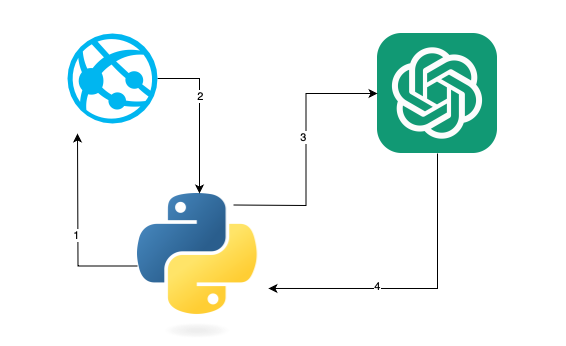
\includegraphics[scale=0.7]{Assets/YOSO.png}
    \caption{YOSO-AI basic workflow}
    \label{fig:yoso}
\end{figure}

\subsection{First public release}
The first pubblic release of ScrapegraphAI  was the version 0.0.1 and it was realead pubblicly on the store pypi on the $17^{th}$ february of 2024. The other two authors and founders of the library are: Marco Perini (Msc mechanical engineering, UniTrento) and Lorenzo Padoan (Msc computer science, Università Ca'​ Foscari Venezia).

Since then the library has started to gain more and more credibility and to be used in scraping pipelines.
\begin{figure}[H]
    \centering
    
\includegraphics[width=0.5\linewidth]{Assets/scrapegraphai_logo.png}
    \caption{Logo of ScrapegraphAI }
    \label{fig:enter-label}
\end{figure}
\subsection{Actual daily usage and numbers of the library}
At the time of writing this thesis (November 2024), the ScrapegraphAI  library has about 100 thousand daily uses with about 1000 unique users.

\begin{figure}[H]
    \centering
    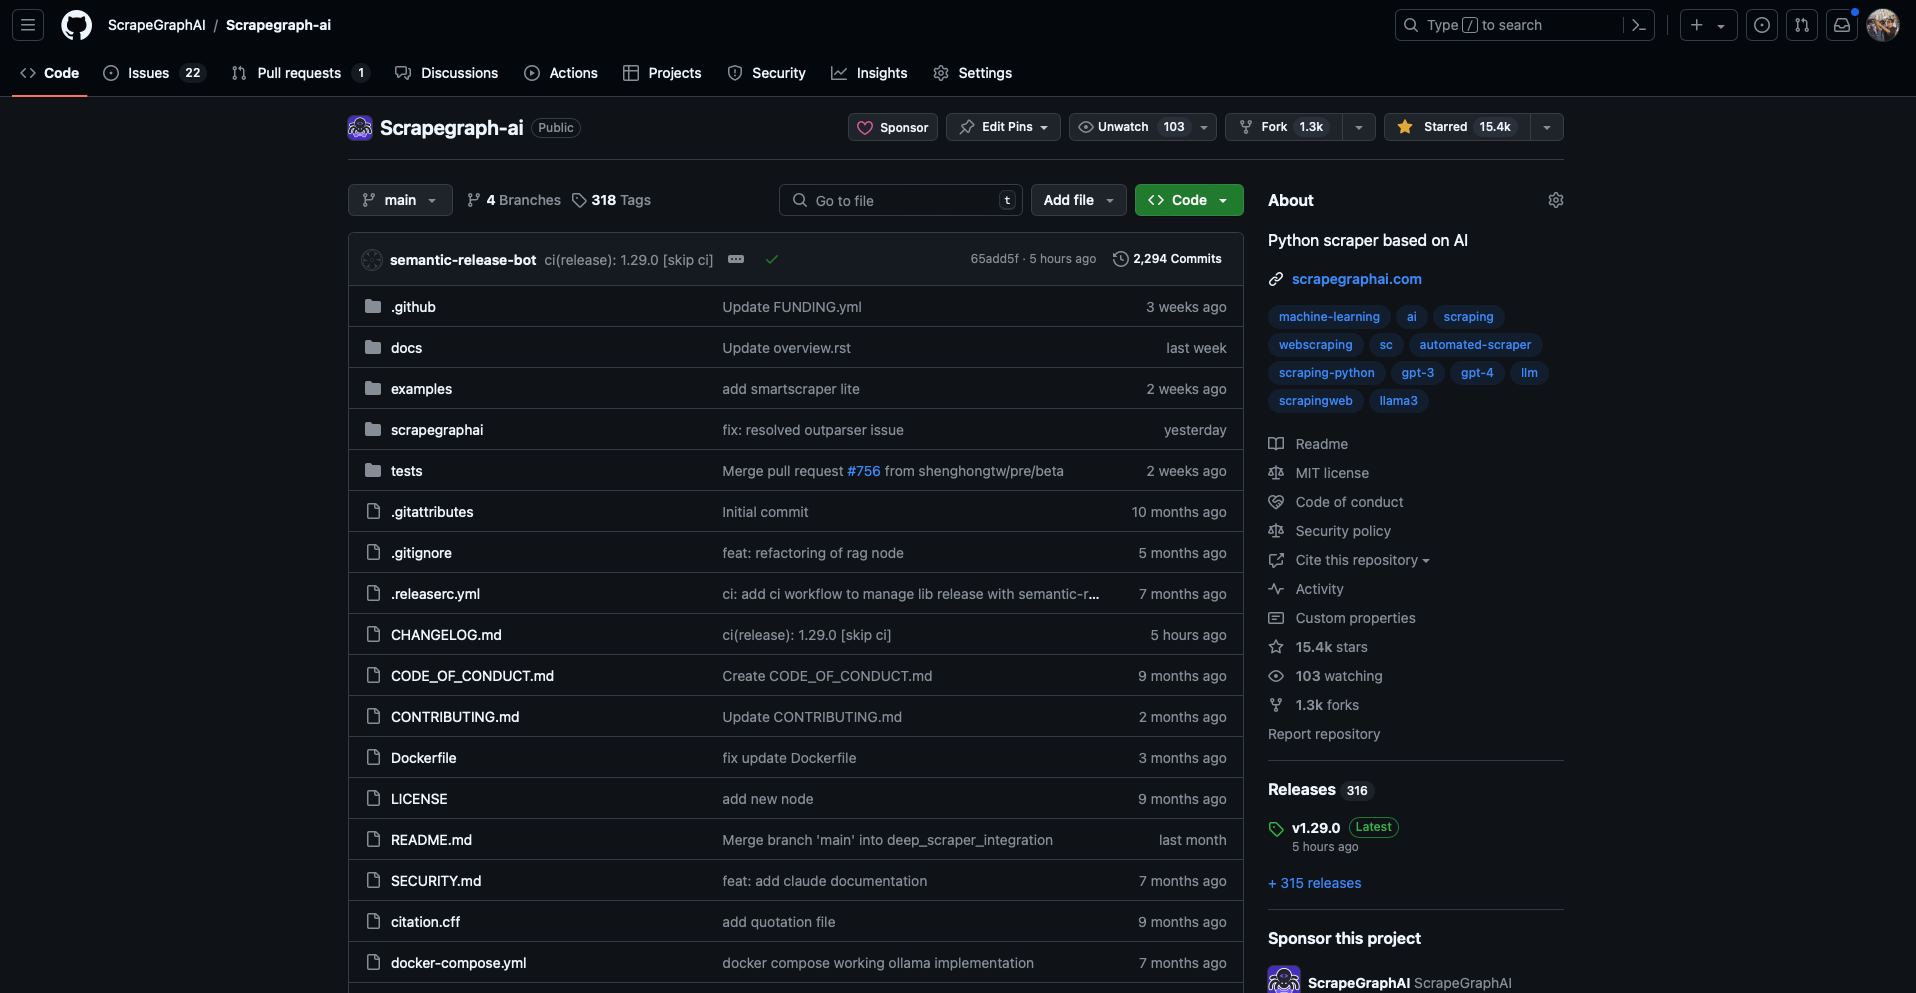
\includegraphics[width=\linewidth]{Assets/Github_home_page.png}
    \caption{Scrapegraph's Github page}
    \label{fig:enter-label}
\end{figure}

\subsection{The power of the open source community}
The role of communities in open-source software (OSS) development has been instrumental in shaping collaborative innovation and sustainability. Communities not only foster shared expertise but also create environments that encourage participation and growth among developers. David and Shapiro (2008) highlight how community-based peer production in OSS provides a unique paradigm for collaboration, emphasizing that such frameworks enable diverse participants to contribute, driven by a blend of intrinsic and extrinsic motivations. Their analysis underscores the significance of understanding the motivational profiles and behavioral patterns of community members, as these aspects directly influence the sustainability and success of OSS projects \cite{David2008}.

Furthering this perspective, Tamburri et al. (2019) discuss the importance of systematically analyzing community patterns to ensure organizational and social health in OSS. Their work introduces tools like Yoshi, designed to measure community characteristics such as structure, engagement, and cohesion. These metrics are critical for identifying potential risks, fostering inclusivity, and ensuring that communities remain dynamic and capable of sustaining long-term development. By mapping community patterns, their research provides actionable insights into improving community governance and preventing project stagnation or failure \cite{Tamburri2019}.

In sum, the power of the community lies in its ability to integrate diverse expertise, maintain resilience through structured governance, and adapt to the evolving landscape of software development. Both studies collectively reinforce that robust community frameworks are not only beneficial but essential for the ongoing success of OSS ecosystems.

\begin{figure}[H]
    \centering
    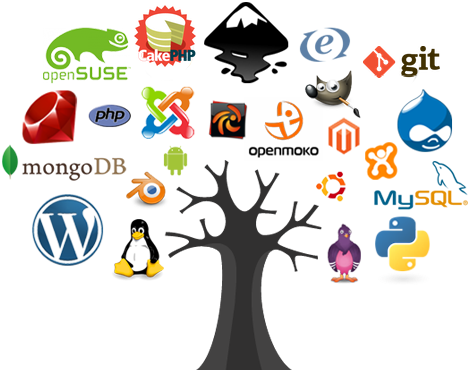
\includegraphics[width=0.5\linewidth]{Assets/community.png}
    \caption{Most famous open source communities}
    \label{fig:enter-label}
\end{figure}

\subsection{Open source events}

The history of Linux exemplifies the transformative power of open-source communities and collaborative events in shaping modern software development. Originating in 1991, Linux was created by Linus Torvalds as a free, open-source operating system kernel. Inspired by the limitations of proprietary systems and the open-source ethos of Unix-like systems, Torvalds shared his project publicly, inviting contributions from developers worldwide. This act of collaboration laid the foundation for what would become one of the most influential open-source projects in history. Over the decades, Linux has evolved through the collective efforts of thousands of contributors, becoming the backbone of diverse technological domains, from servers and cloud infrastructure to mobile operating systems like Android.

Community-driven events, such as PyData, PyCon, and Google Developer Group (GDG) meetups, further highlight how open-source ecosystems flourish. These gatherings serve as catalysts for innovation, knowledge exchange, and skill development. PyData focuses on Python’s role in data science, offering workshops and talks that empower developers to harness its capabilities. PyCon, one of the largest global Python conferences, creates an inclusive platform for exploring cutting-edge applications of Python while nurturing the open-source ethos. GDG events, meanwhile, extend beyond Python, celebrating Google’s open-source technologies, including TensorFlow and Kubernetes, fostering cross-disciplinary collaboration. Together, these events and the historical success of Linux underscore the critical role of open-source communities and initiatives in driving technological progress and empowering developers globally.

\begin{figure}[H]
    \centering
    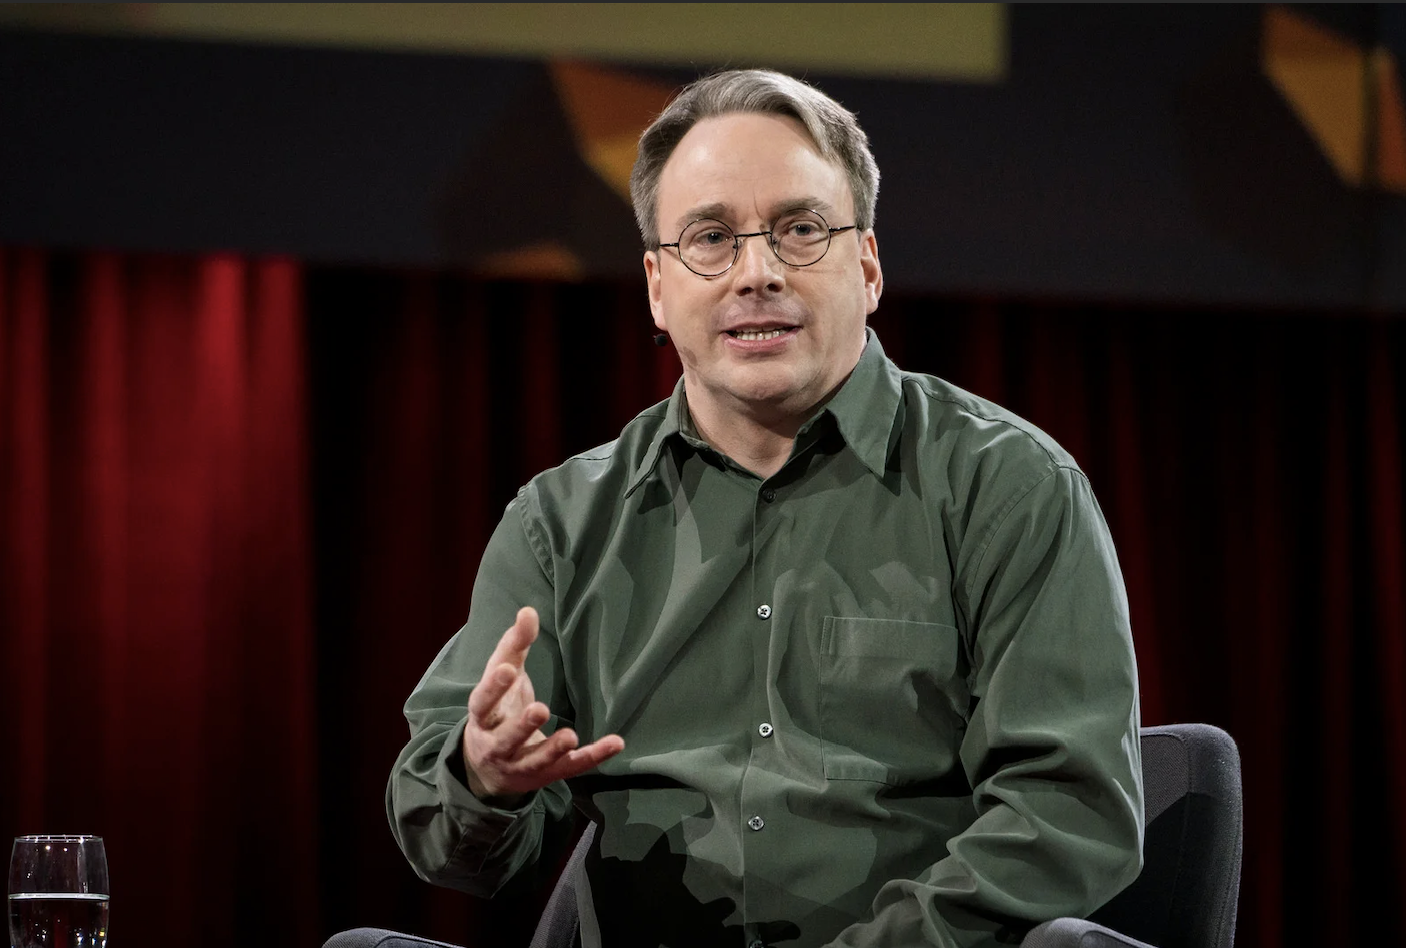
\includegraphics[width=0.5\linewidth]{Assets/torvalds.png}
    \caption{Linus Torvalds, founder of Linux, during a TED talk in 2016}
    \label{fig:enter-label}
\end{figure}

\subsection{Projects created by the community}
Open-source contributors who utilize ScrapegraphAI are a diverse and dynamic group of developers and researchers driven by a shared vision of creating innovative and accessible tools. These individuals often work on projects that range from web scraping pipelines and data analytics platforms to AI-powered applications that leverage real-time information retrieval. By integrating ScrapeGraph's robust capabilities, they unlock new possibilities for scalable and efficient data extraction, benefiting communities in domains such as journalism, e-commerce, and academic research. The library’s modular design, combined with its compatibility with advanced machine learning models, empowers users to build cutting-edge solutions for structured and unstructured data processing.

Additionally, tools like the ScrapegraphAI web dashboard and browser plugin, as depicted in Figures~\ref{fig:web-dashboard} and~\ref{fig:browser-plugin}, provide a seamless interface for developers and non-technical users alike. The web dashboard (Figure~\ref{fig:web-dashboard}) allows users to input their API keys, specify target URLs, define prompts, and optionally provide schemas for data extraction, making it easy to configure and execute scraping tasks. This tool is particularly effective for larger projects requiring detailed configurations or integrations with other software workflows. Similarly, the browser plugin (Figure~\ref{fig:browser-plugin}) streamlines the process by enabling users to select a target website and describe their scraping objectives directly within the browser environment. Its lightweight and intuitive interface empowers users to perform quick, targeted scraping tasks without the need for extensive setup or technical expertise.

These tools exemplify ScrapegraphAI 's mission to democratize web scraping by lowering the technical barriers for users while maintaining advanced features for experts. They also highlight the flexibility of ScrapegraphAI , which can be used in both individual projects and large-scale organizational deployments. With these user-friendly interfaces, developers and researchers can focus on interpreting and utilizing the data rather than spending significant time configuring scraping pipelines.

Moreover, these developers leverage ScrapeGraph’s extensive documentation and active community support to enhance their workflows, ensuring their projects are not only technically sound but also aligned with the principles of transparency and reproducibility. Whether contributing through pull requests, sharing plugins, or publishing tutorials, these users play a pivotal role in expanding the library’s ecosystem. The collaborative ethos of these developers fosters a vibrant ecosystem of shared knowledge, enhancing ScrapeGraph's growth as one of the fastest-growing open-source libraries in the world, according to recent industry rankings. Their work often highlights the importance of ethical data use and the potential of open-source tools to address challenges at scale, paving the way for a future where data accessibility drives impactful change across various sectors.



\begin{figure}[h!]
    \centering
    \includegraphics[width=0.9\textwidth]{Assets/API.png}
    \caption{ScrapegraphAI web dashboard for managing API-based scraping tasks.}
    \label{fig:web-dashboard}
\end{figure}

\begin{figure}[h!]
    \centering
    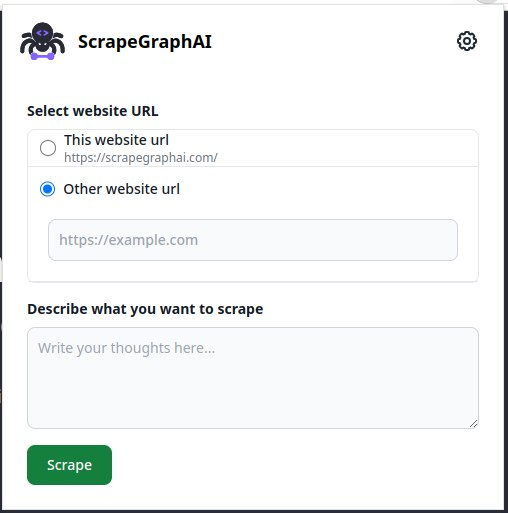
\includegraphics[width=0.75\textwidth]{Assets/tool.jpg}
    \caption{ScrapegraphAI browser plugin for easy, on-the-go scraping setup.}
    \label{fig:browser-plugin}
\end{figure}

\newpage

\section{Thesis structure}
This thesis is organized into several chapters to provide a structured and comprehensive exploration of the research topic.

\begin{itemize}
    \item \textbf{Chapter 1: Abstract} \\
    A concise summary of the thesis, outlining the research objectives, methodology, key findings, and conclusions.

    \item \textbf{Chapter 2: Introduction} \\
    This chapter provides an overview of the role of data in modern technologies, the history and evolution of web scraping, and the challenges posed by current methods. It also introduces the concept of large language models and their potential to revolutionize data extraction techniques. A detailed discussion of the research problem and objectives is included.

    \item \textbf{Chapter 3: Methods and Procedures} \\
    A comprehensive explanation of the methodologies adopted, including neural network architectures, recurrent models, and their application in the context of data scraping and extraction. This chapter also delves into parameter optimization and metrics for evaluating model performance.

    \item \textbf{Chapter 4: Benchmarks and Comparisons} \\
    This chapter compares traditional web scraping techniques with the proposed approach using large language models. Detailed benchmarks, performance metrics, and scalability assessments are provided.

    \item \textbf{Chapter 5: Conclusions and Future Work} \\
    The final chapter summarizes the results achieved, discusses the implications of the findings, and proposes directions for future research, including potential industrial applications and enhancements.

    \item \textbf{Appendices and Bibliography} \\
    Additional resources, datasets, and references are included to support the research and provide further reading materials for interested readers.
\end{itemize}

The structure ensures that readers can easily navigate through the thesis, gaining a clear understanding of the research contributions and their significance.

\chapter{Methods and procedures}
The advancement of artificial intelligence (AI) has been largely driven by the development of artificial neural networks (ANNs), which are inspired by the structure and functionality of the human brain. Neural networks have become a cornerstone of modern AI systems, enabling applications such as natural language processing, computer vision, and autonomous decision-making.

This chapter introduces the theoretical foundations and methodologies underlying neural networks, beginning with the concept of the artificial neuron and its historical development. The chapter also explores the evolution of neural network architectures, including the perceptron and multilayer perceptron, which have been pivotal in shaping modern machine learning algorithms.

By providing a detailed discussion of the mathematical principles, computational techniques, and practical implementations of neural networks, this chapter lays the groundwork for understanding their role in solving complex problems in AI. Visual representations and equations are included to facilitate comprehension and to illustrate the inner workings of these models.
\section{Introduction to neural networks}
The artificial neuron is a mathematical model that was originally proposed in 1943 in \citeauthor{McCulloch1943} \autocite{McCulloch1943}.
Starting in the 1980s, efficient and effective variations of the basic model were published, and around the 1990s these types of techniques became more popular due to the high computing power provided by new computers.

Originally, the proposal was a simplification of the biological neuron model, known as the artificial neuron. It is based on one or more binary inputs and a single binary output. The artificial neuron "activates the output" when a certain number of inputs are active. The connection, or edge, between two neurons or between an input and a neuron is called a link. Each link is associated with a Boolean value that can be either 0 or 1. With this infrastructure, neurons can perform operations based on the traditdional logic operators AND, OR or NOT.

Figure ~\ref{fig:neuronsBasic} depicts the architecture consisting of a single neuron with a single output and one or more inputs.
\begin{figure} [h]
    \centering
    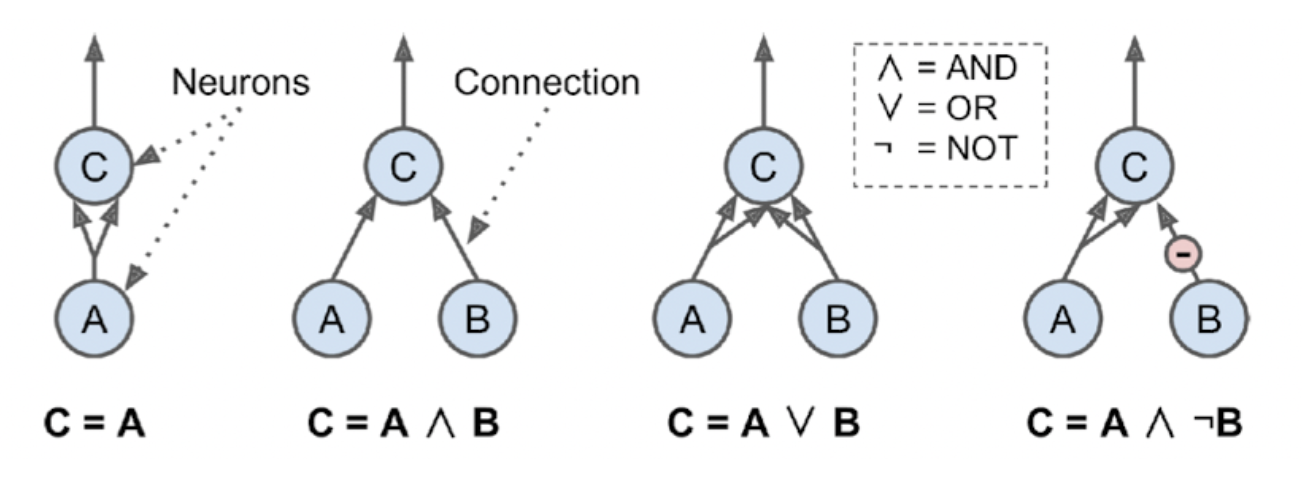
\includegraphics [width=\textwidth,height=\textheight,keepaspectratio] {Assets/Theory_and_methods/unnamed.png}
    \caption{ Scheme of a classical artificial neuron capable of implementing boolean algebra.}
    \label{fig:neuronsBasic}
\end{figure}

\clearpage

\section{The perceptron and multilayer perceptron} \label{percy}
The perceptron is one of the simplest ANN (artificial neural network) architectures. It was invented in 1957 by Frank Rosenblatt. It is based on a neuron called threshold logic unit (TLU) connected to inputs and with only one output link. The inputs and outputs, instead of binary values as in the classical model, are scalar numbers and each link is associated with a weight. The TLU computes a weighted linear combination of the inputs called z $\left(z=w_{1} x_{1}+w_{2} x_{2}+\ldots+w_{n} x_{n}= {\bf x^{t} w}\right)$.

After this input, the step function is applied to the summation represented by z. Formally, this procedure takes place as shown in Eq \eqref{formula} and Figure ~\ref{fig:summatory}.

\begin{equation} 
    h_{w}({\bf x}) = step(z), where \:z = {\bf x^{t} w}
    \label{formula}
\end{equation} 

\begin{figure} [h]
    \centering
   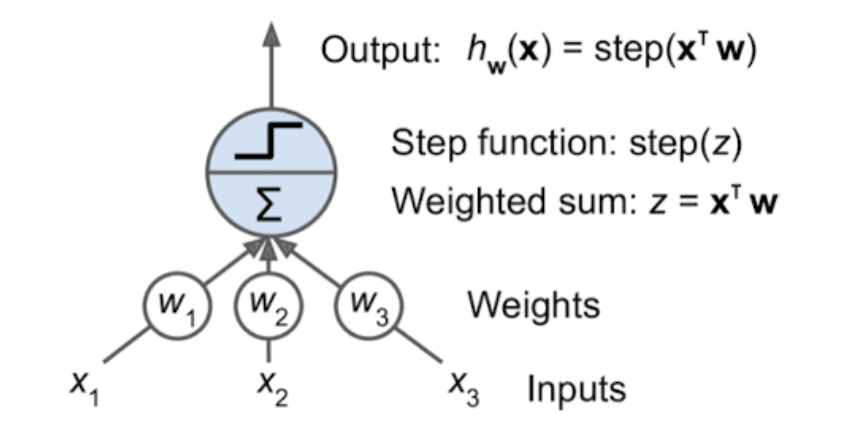
\includegraphics[width=\textwidth,height=\textheight,keepaspectratio]{Assets/Theory_and_methods/unnamed-2.png}
    \caption{Scheme of a Perceptron cell.}
    \label{fig:summatory}
\end{figure}

The most common step function is the heaviside (or step function). In this case,it is used to determine the activation of the neuron based on the output of the linear combination, as shown in Eq \eqref{Heaviside function}: 
\begin{equation} 
    \text { heaviside }(z)=\left\{\begin{array}{l}
    0 \text { if } z<0 \\
    1 \text { if } z \geq 0
    \end{array}\right.
    \label{Heaviside function}
\end{equation} 

A single TLU can be used for simple binary classification. If the input exceeds a certain threshold, it is associated with one category, otherwise, if it is lower than said threshold, it is associated with the other category.

A so called perceptron simply consists of a single layer of TLUs, where each TLU is connected to all of the inputs.

It is possible to extend this architecture by stacking more layers, where each output of the neurons of a given layer is connected to each input of the neurons in the next layer.This new architecture is called a Multilayer Perceptron (MLP), where the layers between the input and output layers are called  hidden layers.
 (Figure ~\ref{fig:Perceptron}).

\begin{figure} [h]
    \centering
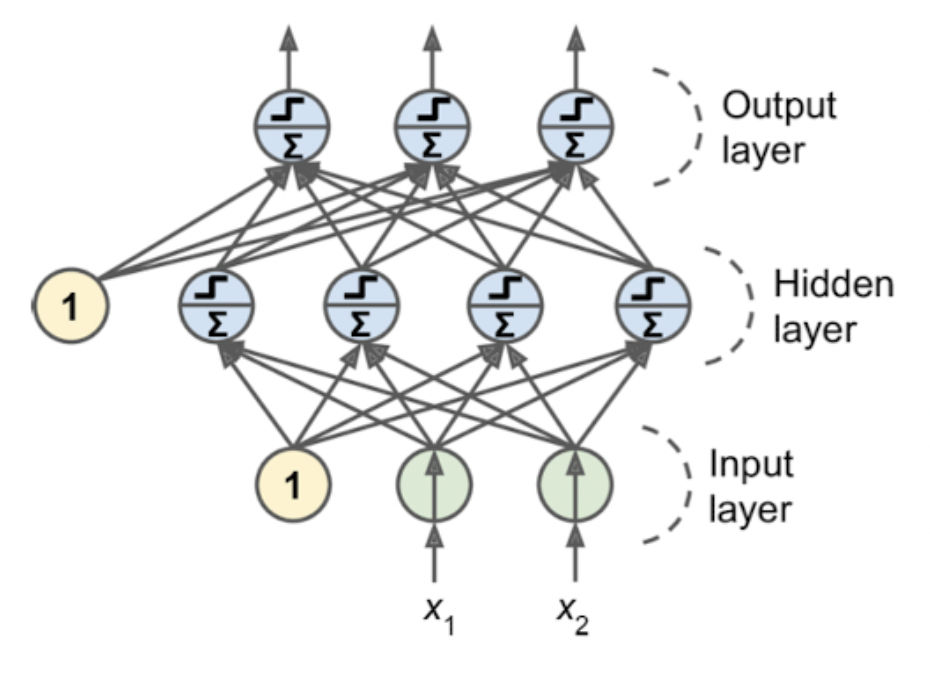
\includegraphics[width=\textwidth,height=\textheight,keepaspectratio]{Assets/Theory_and_methods/unnamed-3.png}
    \caption{Figure 3: multi layer perceptron.}
    \label{fig:Perceptron}
\end{figure}

When all neurons in a layer are connected to every neuron in the previous layer, the layer is called a fully connected layer or dense layer.
Eq \eqref{bohfoormulas}. represents this type of model.
\begin{equation} 
   h_ {W,b} ({\bf X}) = \phi({\bf XW + b})
    \label{bohfoormulas}
\end{equation} 

In this equation:
\begin{itemize}
    \item \textbf{X} represents the input feature matrix.
    \item \textbf{W} represents the matrix of weights. It contains all the weights except the bias neuron.

    \item \textbf{b} is a vector that contains all the weights between the bias neuron and the artificial neuron (it contains the distortions between the results and reality).
    \item \textbf{$\phi$} is called an activation function. Which is the step function in the case of the Multilayer Perceptron.
\end{itemize}

Regarding the learning phase, a learning rule that was largely inspired by Hebb's rule, introduced in \citeauthor{Morris1999} \autocite{Morris1999}, is used. In the text it is said that, in nature, when a biological neuron is activated, it consequently activates or triggers another neuron, the connection between the two becomes greater. The perceptron is trained with a variant of this concept that takes into account the errors made by the network when making predictions. The learning rule reinforces connections that help reduce error and reduces those that contribute to increased error. Eq \eqref{bohfoormula} represents the the learning rule.

\begin{equation} 
   w_ {i, j} ^{(next step)} = w _{i, j }+ \eta( y _{j} - ŷ_{j}) x_{i} 
    \label{bohfoormula}
\end{equation}

\begin{itemize}
    \item $w _{i, j}$ is the connection weight between to given neurons.
    \item $x_{i} $ is the value of the input.
    \item $ŷ _{j}$ is the interpolated value of the output.
    \item $y_{j}$ is the observed value of the output.
    \item $\eta$ is the learning rate.
\end{itemize}
\section{Backpropagation and parameter optimization} \label{backprop}
Error backpropagation is an algorithm used for training artificial neural networks, which is used as a method for stochastic gradient descent and thus enables error reduction in the learning process. The term backpropagation refers only to the algorithm for computing the gradient, not to describe how the gradient is used.

The learning phase therefore consists in finding the optimal parameters that create the best model, and an iterative approach is used to do this by gradually modifying the parameter values with respect to the previous iteration.

This training mechanism starts with random initialization of the parameters and is carried out using input-output pairs until a minimum of the cost function, which is responsible for calculating the error, is reached. Each iteration is called an epoch.
The optimization procedure is as follows:
\begin{itemize}
    \item The weights and biases of the network are initialized with random values.
    \item These parameters are iteratively optimized. This phase consists in 4 subphases:
    \begin{itemize}
        \item The model prediction is calculated using the current parameters.
        \item The cost function, that drives the optimization process, is applied to the obtained output with respect to the expected output.
        \item The gradient, which will be used to determine how to tweak the parameters, is calculated with respect to the cost function through the process of backpropagation.
        \item The parameters are updated. 
    \end{itemize}
\end{itemize}

These four steps can be repeated for an arbitrary number of iterations, and the process is usually stopped when a local minimum is reached.
\clearpage 
\section{Hyperparameters} \label{hyperdescrp}
While the values of a neural network’s parameters, namely its weights and biases, are defined by its training process, there’s a set of different parameters, called hyperparameters, that are not optimized by the learning process. 
The hyperparameters of a neural network define its architecture and the characteristics of its learning phase. They act as factors, external to the learning phase, that have an impact on the model’s performance.
The most important hyperparameters are the following:
\begin{itemize}
    \item \textbf{Batch}
    \\When Stochastic Gradient Descent (SGD) is used, the parameters are updated after each sample of the dataset is evaluated in the training phase. This approach is considered significantly noisy since the gradient descent direction derived by one sample might differ from the direction derived from other samples, significantly increasing the variance across the different iterations of the learning process.
    \\Generally speaking, the model gets updated after a specific number of samples has been processed. This is known as the batch size of samples.  SGD can therefore be seen as having a batch size of one.
    In addition to being less noisy, the use of batch sizes greater than one results in reduced training times if paired with the use of GPUs or other specialized hardware. Moreover, the optimization towards a minimum will likely be less erratic than in the case of SGD, increasing the chances of actually converging.

    \item \textbf{Epoch}
    \\An epoch in machine learning means one complete pass of the training set through the algorithm, that is, its propagation through the network’s architecture. Normally an epoch is divided into one or more batches. The number of epochs and batches per epoch are both integers.
    \\There’s no limit to the amount of epochs to use in the training process, which can thus take up an arbitrary amount of time. To stop the algorithm from running, a fixed number of epochs can be used. Alternatively, early-stopping can be used, which consists of stopping the training as soon as the validation error stops showing significant improvements after a predetermined number of epochs, referred to as patience. As a consequence, the number of epochs can be set to a big integer to give ample room for the training to take place, while relying on early-stopping to stop when appropriate.
    \item \textbf{Number of hidden layers}
    \\As explained in chapter ~\ref{percy}, the number of hidden layers is determined by the amount of layers between the input and output layers.
    \item \textbf{Number of neurons per layer}
    \\The number of neurons in input and output layers is determined by the type of the input and output necessary for the task at hand. For the hidden layers, on the other hand, it used to be common to structure them into a pyramid-shaped, with fewer and fewer neurons at each layer. For instance, a neural network could have 3 hidden layers, the first one with 300 neurons, the second with 200 neurons and the last with 100. 
    This practice, however, is not used anymore because it’s been empirically proven that using the same number of neurons in all hidden layers performs just as well in most cases.
    \item \textbf{Learning rate}
    \\It determines the step size to be used during the optimization process between a training iteration and the next. It can therefore result in the training process stalling, due to a very small learning rate that hinders progress towards a minimum, or it can result in a model that converges too quickly to a local minimum that yields suboptimal results, making it one of the most important hyperparameters.
    \\One way to find a good learning rate is to train the model for a few hundred iterations starting with a learning rate (for example 10-5) and gradually increasing it up to a large value (for example $10^{\frac{\log \left( 10^{6}\right)  }{500} }$). This is done multiplying the learning rate by a constant factor at each iteration (like ). As a  consequence, the loss should drop more and more quickly when comparing different runs of the training phase that use increasingly bigger learning rates. The ideal learning rate will be one that strikes a balance between the training time and the model’s ability to actually converge to a minimum.
    
\end{itemize}
\section{Training test, validation test and testing set}
The training, validation and testing set are derived by splitting the dataset in three subsets. The first one (training dataset) is exclusively used in the training phase during which the model’s parameters are defined.
The validation set instead is used for evaluating a given model’s evolving performance during the training phase, by using data that it hasn’t used for the training itself.
\\Lastly, the testing set is used for evaluating the model once it has been completely trained. 
\\Technically speaking, the same set could be used for both testing and validation, but it’s good practice to use two separate ones.


\section{Metrics}
\subsection{Coefficient of determination (R2)}
The coefficient of determination \autocite{RossStat} is the proportion of the variation of the response variable that can be explained through the independent variables of the model.
In order to define it mathematically, it is necessary to introduce a few concepts, like the definition residuals, residual sum of squares and the total sum of squares.
\\The residuals are the difference between the observed data of the target variable and the respective values predicted by the model. Therefore, the residual sum of squares (Eq. \eqref{ssres}) is the sum of all residuals in which each residual has been squared.

\begin{equation}
S S_{\mathrm{res}}=\sum_{i}\left(y_{i}-f_{i}\right)^{2}=\sum_{i} e_{i}^{2}
\label{ssres}
\end{equation}
The total sum of squares (Eq. \eqref{sstot}) is the sum of the squared differences between the observed data of the target variable and their mean.

\begin{equation}
S S_{\mathrm{tot}}=\sum_{i}\left(y_{i}-\bar{y}\right)^{2}
\label{sstot}
\end{equation}
Knowing these concepts, the coefficient of determinations can be described as in Eq \eqref{r2}. Its value ranges between zero and one.
\begin{equation}
R^{2}=1-\frac{S S_{\mathrm{res}}}{S S_{\mathrm{tot}}}
\label{r2}
\end{equation}

\subsection{Root mean squared error (RMSE)}
The root mean squared error \autocite{RossStat} is one of the most commonly used metrics for evaluating the quality of predictions. It shows how far predictions fall, relative to observed values, using Euclidean distance. It is a measure of spread out the residuals are, in that it is determined by how concentrated the data is around the line of best fit.
\\The root mean square error can be calculated using Eq \eqref{rmse}
\begin{equation}
R M S E=\sqrt{\frac{\sum_{i=1}^{N}\|y(i)-\hat{y}(i)\|^{2}}{N}},
\label{rmse}
\end{equation}

In this equation y is the real value and ŷ  is the interpolated value.

\subsection{Mean Absolute Error MAE}
The MAE is one of the many metrics that allow for an assessment of the performance  of a machine learning model. It’s the average of the absolute error as shown in the Eq \eqref{mae}.

\begin{equation}
m a e=\frac{\sum_{i=1}^{n} a b s\left(y_{i}-\lambda\left(x_{i}\right)\right)}{n}
\label{mae}
\end{equation}

\clearpage

\section{Recurrent neurons (RNN) and layers}
So far the theoretical part of the thesis has been focused on artificial neural networks where the activation link is monodirectional and propagates its values to the next layer, or to the output of the model in the case of the output layer. This type of model is called feedforward neural network.

For the purposes of this thesis, however, a different type of mathematical model called recurrent neural network (RNN) was used. In it, the output of the neuron itself is used as an input for the next time step, thus creating a loop on the node (Figure ~\ref{fig:Recurrent_neurons}).
Generally speaking, RNNs use the logistic curve as their activation function, but the hyperbolic function and ReLU can still be used.

It has been found that the simple introduction of this mechanism increases the performance of t neural networks when they are used as regression models, especially when the data is correlated over time. 

\begin{figure} [h]
    \centering
    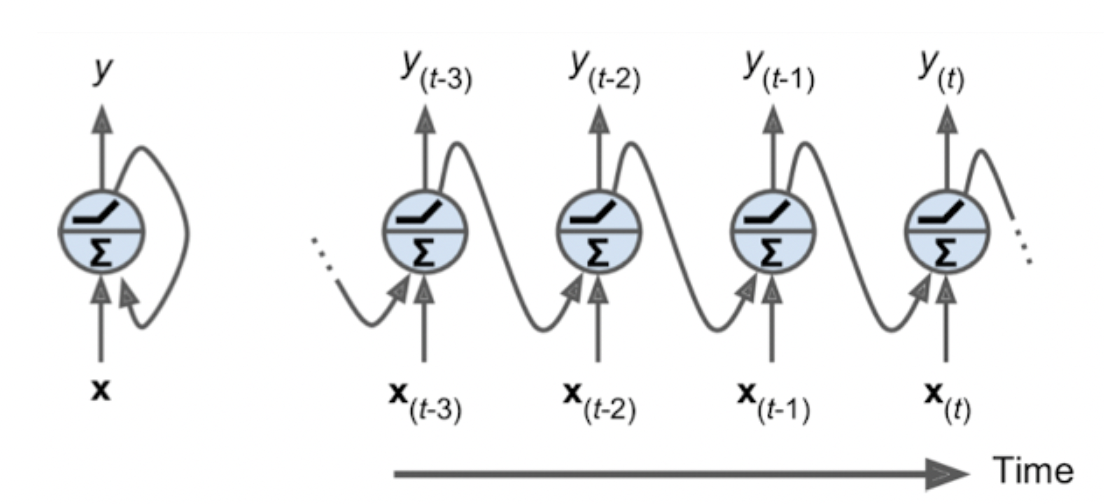
\includegraphics[width=\textwidth,height=\textheight,keepaspectratio]{Assets/Theory_and_methods/unnamed-6.png}
    \caption{Recurrent neurons.}
    \label{fig:Recurrent_neurons}
\end{figure}

Starting from a single RNN neuron it is possible to easily create one or more layers (Figure ~\ref{fig:RNN_multi_layer}). In more advanced models instead of using the output of a single neuron as an input for the next time step, the entire output of the layer can be used.

\begin{figure} [h]
    \centering
    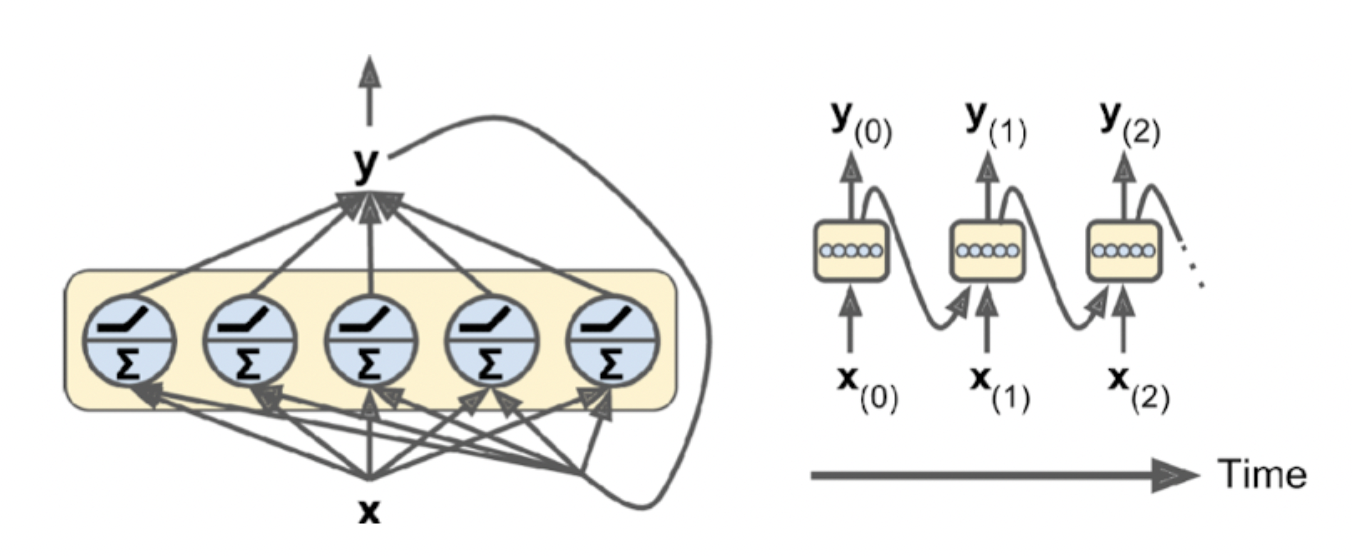
\includegraphics[width=\textwidth,height=\textheight,keepaspectratio]{D) IMAGES/Theory_and_methods/unnamed-7.png}
    \caption{RNN architecture with multiple neurons.}
    \label{fig:RNN_multi_layer}
\end{figure}

Each recurrent neuron has two types of weights: one for the input x(t) and the other for the output at the previous step $y_{(t-1)}$ . These two types of weights are called wx and wy, respectively. The output vector of the model is shown in Eq. \eqref{longformula}:

\begin{equation} 
   {\bf y }(t) = {\bf \phi}({\bf W}_{x}^{T} x (t) +{\bf W} _{y} ^{T} {\bf y} _{(t-1)} + {\bf b}) 
    \label{longformula}
\end{equation}

where ${\bf W}_x^T$  s the transposed version of matrix ${\bf W}_x$.

Jus like with feedforward neural network, it is possible to compute a single-step output of any given layer for  an entire batch of values by putting them all in the input matrix $X_{(t)}$ via the Eq. \eqref{longlongformula}:

\begin{equation} 
   {\bf Y} _{(t)} = {\bf \phi}({\bf X}_{(t)} {\bf W} _x + {\bf Y} _{(t-1)}{\bf W}_y + {\bf b}) = {\bf \phi}([{\bf X }_{(t)} , {\bf Y}_{(t-1)} ] {\bf W}  + {\bf b}) \: with \: {\bf W} = [{\bf W}_x ,{\bf W}_y ]^T
    \label{longlongformula}
\end{equation}

In this equation: 

\begin{itemize}
    \item ${\bf Y}_{(t)}$ is an m x $n_{neurons}$ matrix that contains the output of the layer at a given step t for each instance in the -batch (m is the number of instances, n neurons is the number of neurons).
    \item $X (t)$ is an m x n inputs matrix containing the inputs for all instances.
    \item ${\bf W}_x$ is a  $n_{inputs} \:x\: n_{neurons}$ matrix containing the connection weights for the inputs at a time t.
    \item ${\bf W}_y $ is a $n_{neurons} \:x\: n_ {neurons}$ matrix  containing the connection weights for the outputs at a previous step.
    \item ${\bf b}$ is a vector of size n, equal to the number of neurons, containing the bias of each neuron.
    Regarding the second part of the equation (compact notation):
     \item ${\bf W}$ is the vertical concatenation of the matrices ${\bf W}_x$ and ${\bf W}_y$.
    \item $[{\bf X}_{(t)}, {\bf Y}_{(t-1)}]$ represents the vertical concatenation of the matrices ${\bf X}_{(t)}$ and ${\bf Y}_{(t-1)}$.
\end{itemize}

\section{Memory Cells and long short memory term network}

\subsection{Introduction to LSTM and limits of RNN}
When using an RNN, some information is lost  or forgotten at each step. After a certain number of iterations the state of the RNN no longer contains any trace of information from the first inputs. In fact, the neurons' memory typically does not go beyond 10 steps.

It is, however, possible to extend the model in order to add memory beyond 10 steps, which is useful for doing time series forecasting, of both univariate and multivariate in nature.

\subsection{LSTM cell} \label{lstmcell}
The Long Short-Term Memory (LSTM) cell was introduced in 1997 in \citeauthor{LSTM} \autocite{LSTM}.
It offers improved performance and results compared to a other types of cells, such as RNN cells. In fact, LSTM neural networks have shorter convergence times and are also able to keep track of medium to long term dependencies in time series data such as trend and seasonality.

\begin{figure} [h]
    \centering
    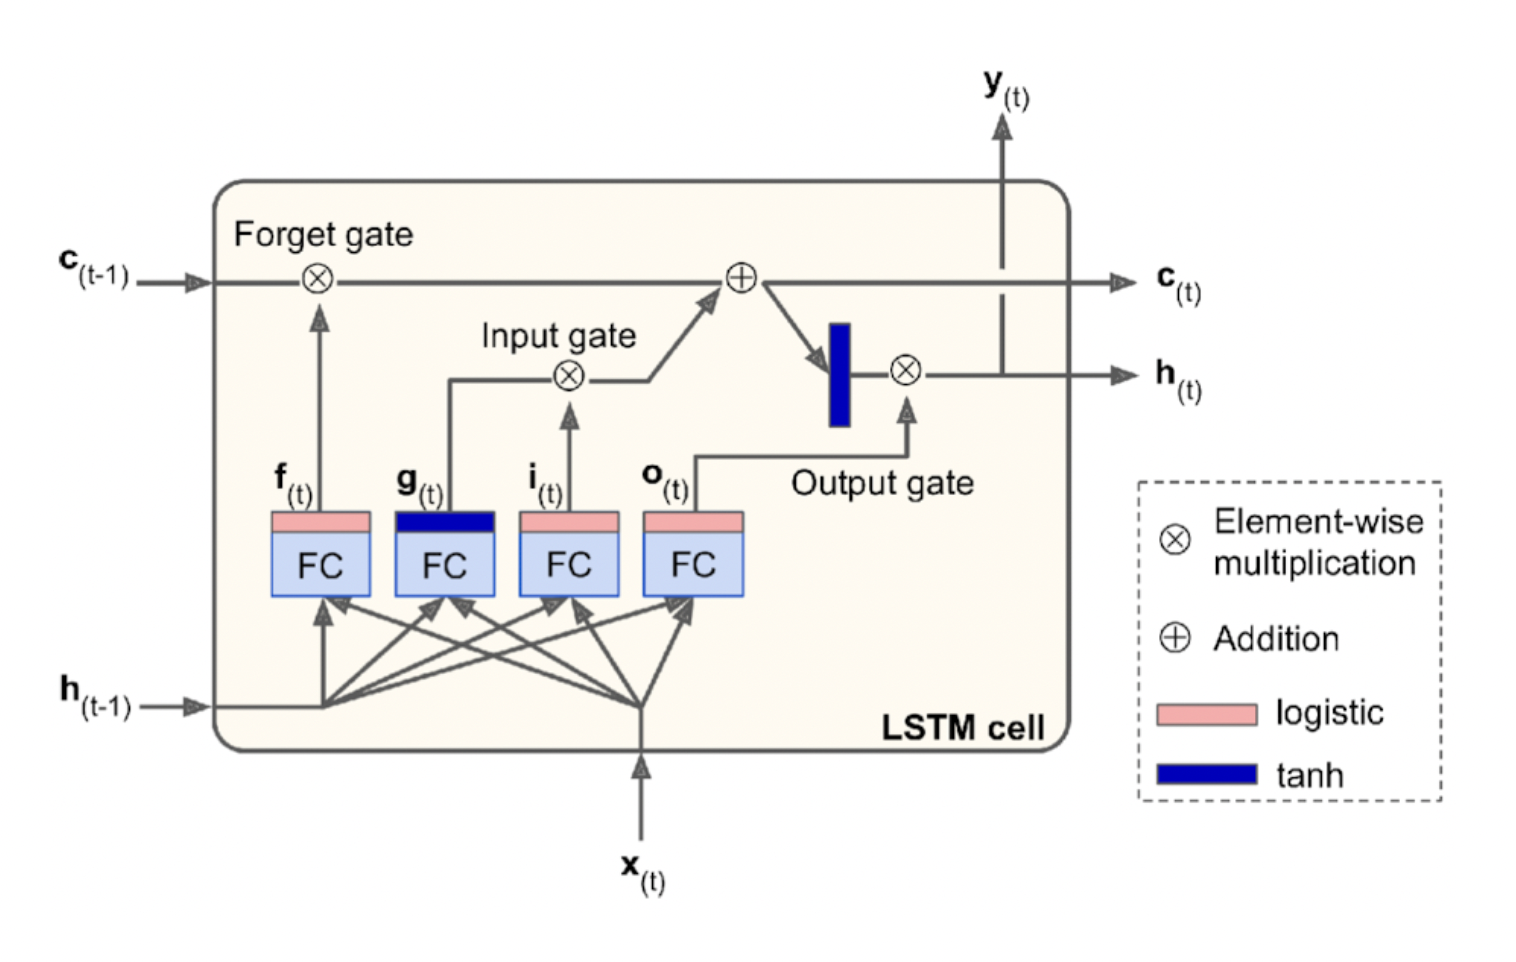
\includegraphics[width=\textwidth,height=\textheight,keepaspectratio]{Assets/Theory_and_methods/unnamed-8.png}
    \caption{LSTM cell.}
    \label{fig:LSTM_cell}
\end{figure}

As can be see in figure ~\ref{fig:LSTM_cell}, the cell works exactly like a classic cell, except that the state is split into 2 vectors: ${\bf h}_{(t)}$ and ${\bf c}_{(t)}$, which represent respectively the short term state and the long term state.
\begin{itemize}
    \item The main component is the one that deals with the output ${\bf g}_{(t)}$. Its activation function is a hyperbolic tangent. It deals with analyzing the input ${\bf g} {(t)}$ and the previous state ${\bf h}_{(t-1)}$. In a basic cell this would be the only component and its output would go directly to ${\bf y }_{(t)}$ and ${\bf h} _{(t)}$. In contrast, in LSTM cells the output of this cell is processed such that the most important information in the long-term state is kept and the rest of the data that is not useful is dropped. 
    \item
        The other three components are called gate controllers, because they use the logistic function as the activation function and thus their output range is between 0 and 1. Their roles are as follows: 
        \begin{itemize}
            \item ${\bf f}_{(t)}$ is called the forget gate, which defines which part of the long-term memory is to be erased. 
            \item ${\bf i}_{(t)}$ is the input gate, which determines which part of g (t) should be added to the long-term memory.
            \item ${\bf o}_{(t)}$ is called the output gate and controls which part of long-term memory should be read and added to the output, both for ${\bf h}_{(t)}$ and ${\bf y}_{(t)}$.
        \end{itemize}
\end{itemize}


Therefore, an LSTM cell can learn to recognize particularly important inputs, add them the long-term state, and store them internally until it is needed. This explains why this model has been more successful in capturing long-term patterns when it comes to time series.

 Eq. \eqref{systemformula} contains the mathematical construction of an LSTM cell.

\begin{equation} 
    \begin{array}{l}
    \mathbf{i}_{(t)}=\sigma\left(\mathbf{W}_{x i}^{\top} \mathbf{x}_{(t)}+\mathbf{W}_{h i}^{\top} \mathbf{h}_{(t-1)}+\mathbf{b}_{i}\right) \\
    \mathbf{f}_{(t)}=\sigma\left(\mathbf{W}_{x f}^{\top} \mathbf{x}_{(t)}+\mathbf{W}_{h f}^{\top} \mathbf{h}_{(t-1)}+\mathbf{b}_{f}\right) \\
    \mathbf{o}_{(t)}=\sigma\left(\mathbf{W}_{x o}^{\top} \mathbf{x}_{(t)}+\mathbf{W}_{h o}^{\top} \mathbf{h}_{(t-1)}+\mathbf{b}_{o}\right) \\
    \mathbf{g}_{(t)}=\tanh \left(\mathbf{W}_{x g}^{\top} \mathbf{x}_{(t)}+\mathbf{W}_{h g}^{\top} \mathbf{h}_{(t-1)}+\mathbf{b}_{g}\right) \\
    \mathbf{c}_{(t)}=\mathbf{f}_{(t)} \otimes \mathbf{c}_{(t-1)}+\mathbf{i}_{(t)} \otimes \mathbf{g}_{(t)} \\
    \mathbf{y}_{(t)}=\mathbf{h}_{(t)}=\mathbf{o}_{(t)} \otimes \tanh \left(\mathbf{c}_{(t)}\right)
    \end{array}
    \label{systemformula}
\end{equation}
The meanings of the terms in the equations are as follows:

\begin{itemize}
    \item  ${\bf W}_{xi} , {\bf W}_{xf} , {\bf W}_{x0}$ and $\: {\bf W}_{xg}$ are the matrices that contain the weights for each of the four components with respect to their connection to the input vector ${\bf x}_{(t)}$.
   
    \item ${\bf W}_{hi} , {\bf W}_{hf} , {\bf W}_{h0}$ and ${\bf W}_{hg}$ are the matrices that contain the weights for each of the four components with respect to their connection to the short term memory state ${\bf h}_{(t-1)}$.
    
    \item ${\bf b}_{i} , {\bf b}_{f}, {\bf b}_{0},$  and ${\bf b}_{g}$ are the bias values for each of the four components. 

\end{itemize}

\clearpage

\subsection{Other cells: Dense cells and GRU cells}
The Gated Recurrent Unit (GRU) cells were first proposed in 2014 by \citeauthor{DBLP:journals/corr/ChoMGBSB14} \autocite{DBLP:journals/corr/ChoMGBSB14}. GRU cells are a simplified version of LSTM cells, which seem to work more efficiently. The major simplifications are as follows:

\begin{itemize}
    \item The state vectors (long and short term) are combined into a single vector ${\bf h}_{(t)}$.
    \item A single gate controller ${\bf z}_{(t)}$ controls both the forgotten gate and the input gate.
    \item There is no output gate. Instead, the entire state vector is used as the output.
\end{itemize}
The schematic of the GRU cell is available in figure. ~\ref{fig:GRU_cell}:
\begin{figure} [h]
    \centering
    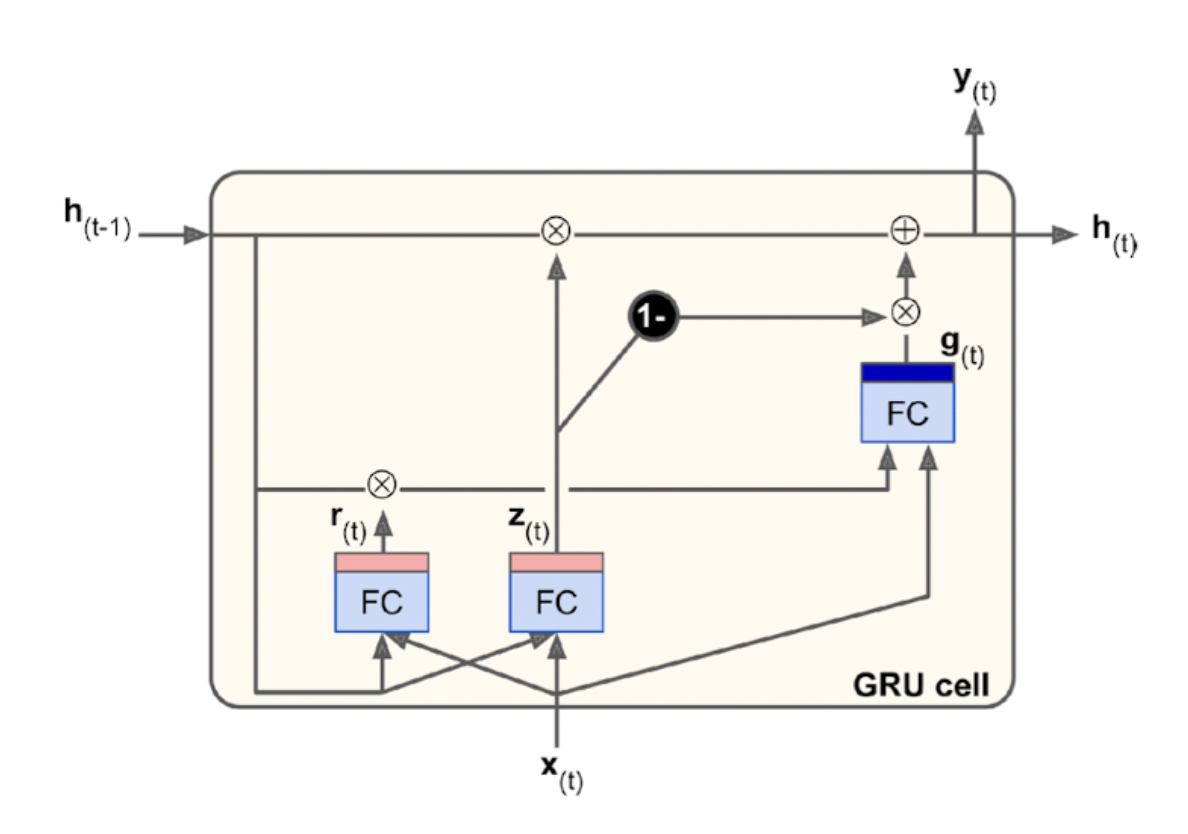
\includegraphics[width=\textwidth,height=\textheight,keepaspectratio]{Assets/Theory_and_methods/unnamed-9.png}
    \caption{GRU cell.}
    \label{fig:GRU_cell}
\end{figure}

\clearpage
\section{Introduction to LLMs}
\subsection{Generative AI Design Cycle}
The design cycle of Generative AI (GenAI) encompasses several critical stages, each integral to the development and deployment of effective generative models. As outlined in Hadi et al. \cite{hadi2024}, this cycle can be broadly categorized into four phases: problem definition, model selection or development, adaptation and alignment, and deployment and optimization.

In the initial phase, the problem definition sets the scope of the target application. Developers determine whether the model will perform single or multiple tasks, which directly influences the design and training approach. Following this, the model selection phase involves deciding between using pre-existing models like transformers or training a new model from scratch. Depending on the requirements, developers may employ general techniques such as RNNs or transformers, or refine models through advanced methods like generative adversarial networks or diffusion models.

The adaptation and alignment phase is iterative, focusing on techniques such as prompt engineering and fine-tuning. These processes ensure the model's output aligns with the desired outcomes. For example, developers might implement zero-shot or few-shot learning to optimize model performance based on specific tasks.

Finally, in the deployment and optimization phase, the trained model is integrated into real-world applications. This phase emphasizes continual refinement to enhance model efficiency and accuracy. Optimization strategies ensure the model performs reliably in diverse scenarios while adhering to ethical and computational constraints.

By iteratively addressing these stages, the Generative AI design cycle facilitates the creation of robust, adaptable, and application-specific models capable of generating high-quality outputs across various domains.
\subsection{Attention is all you need}
The Transformer model introduced a groundbreaking approach to natural language processing (NLP) by eliminating the reliance on recurrence and convolution, as seen in earlier models like recurrent neural networks (RNNs) and convolutional neural networks (CNNs). Instead, Transformers utilize attention mechanisms exclusively, enabling parallel computations and faster training times \cite{vaswani2017attention}.

At the heart of the Transformer lies the \textit{Scaled Dot-Product Attention}, as shown in Figure~\ref{fig:scaled_attention}. This mechanism computes the attention scores by combining query (Q), key (K), and value (V) vectors. The scores are scaled to mitigate large gradients, normalized using a softmax function, and optionally masked for sequential tasks. Building on this, the \textit{Multi-Head Attention} mechanism, depicted in Figure~\ref{fig:multi_head_attention}, enhances the model's ability to capture diverse relationships within the input by projecting Q, K, and V into multiple subspaces and concatenating the results.

The overall architecture of the Transformer, illustrated in Figure~\ref{fig:transformer_architecture}, consists of stacked encoder and decoder layers. Each encoder layer incorporates multi-head attention and feed-forward components, while the decoder introduces masked attention to support autoregressive tasks. To address the lack of intrinsic sequence awareness, positional encodings are added to the input embeddings. This combination of components provides a robust framework for various applications, including text generation and machine translation.

\begin{figure}[h!]
    \centering
    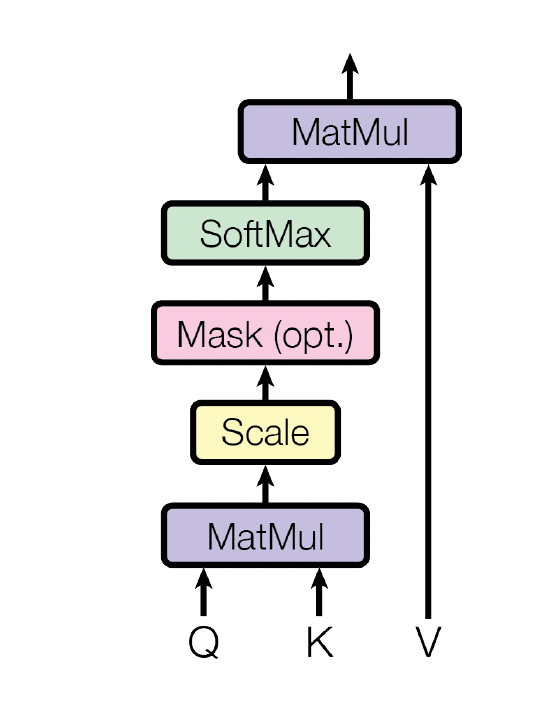
\includegraphics[width=0.55\textwidth]{Assets/scaled_dot_product_attention.png}
    \caption{Scaled Dot-Product Attention mechanism. Source: \cite{vaswani2017attention}}
    \label{fig:scaled_attention}
\end{figure}

\begin{figure}[h!]
    \centering
    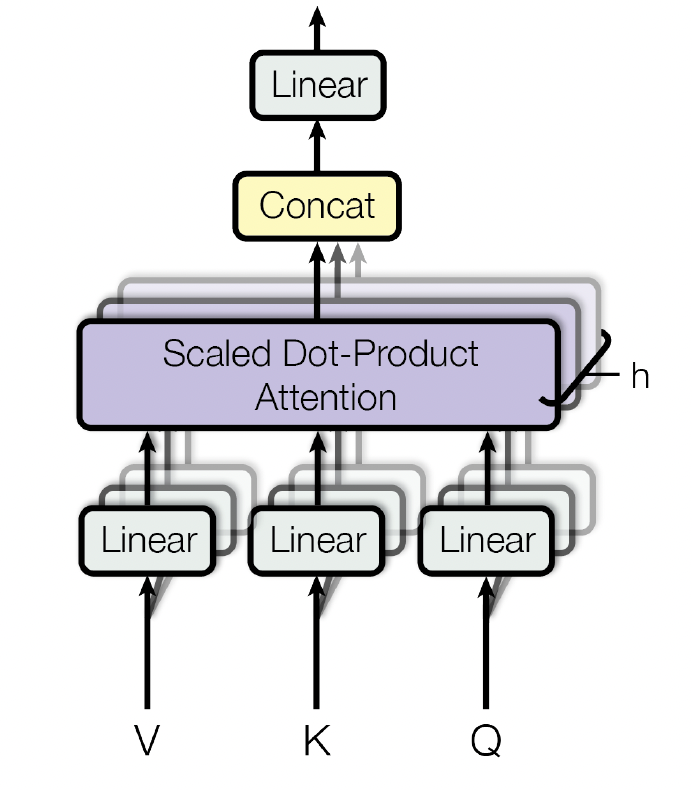
\includegraphics[width=0.55\textwidth]{Assets/multi_head_attention.png}
    \caption{Multi-Head Attention mechanism. Source: \cite{vaswani2017attention}}
    \label{fig:multi_head_attention}
\end{figure}

\begin{figure}[h!]
    \centering
    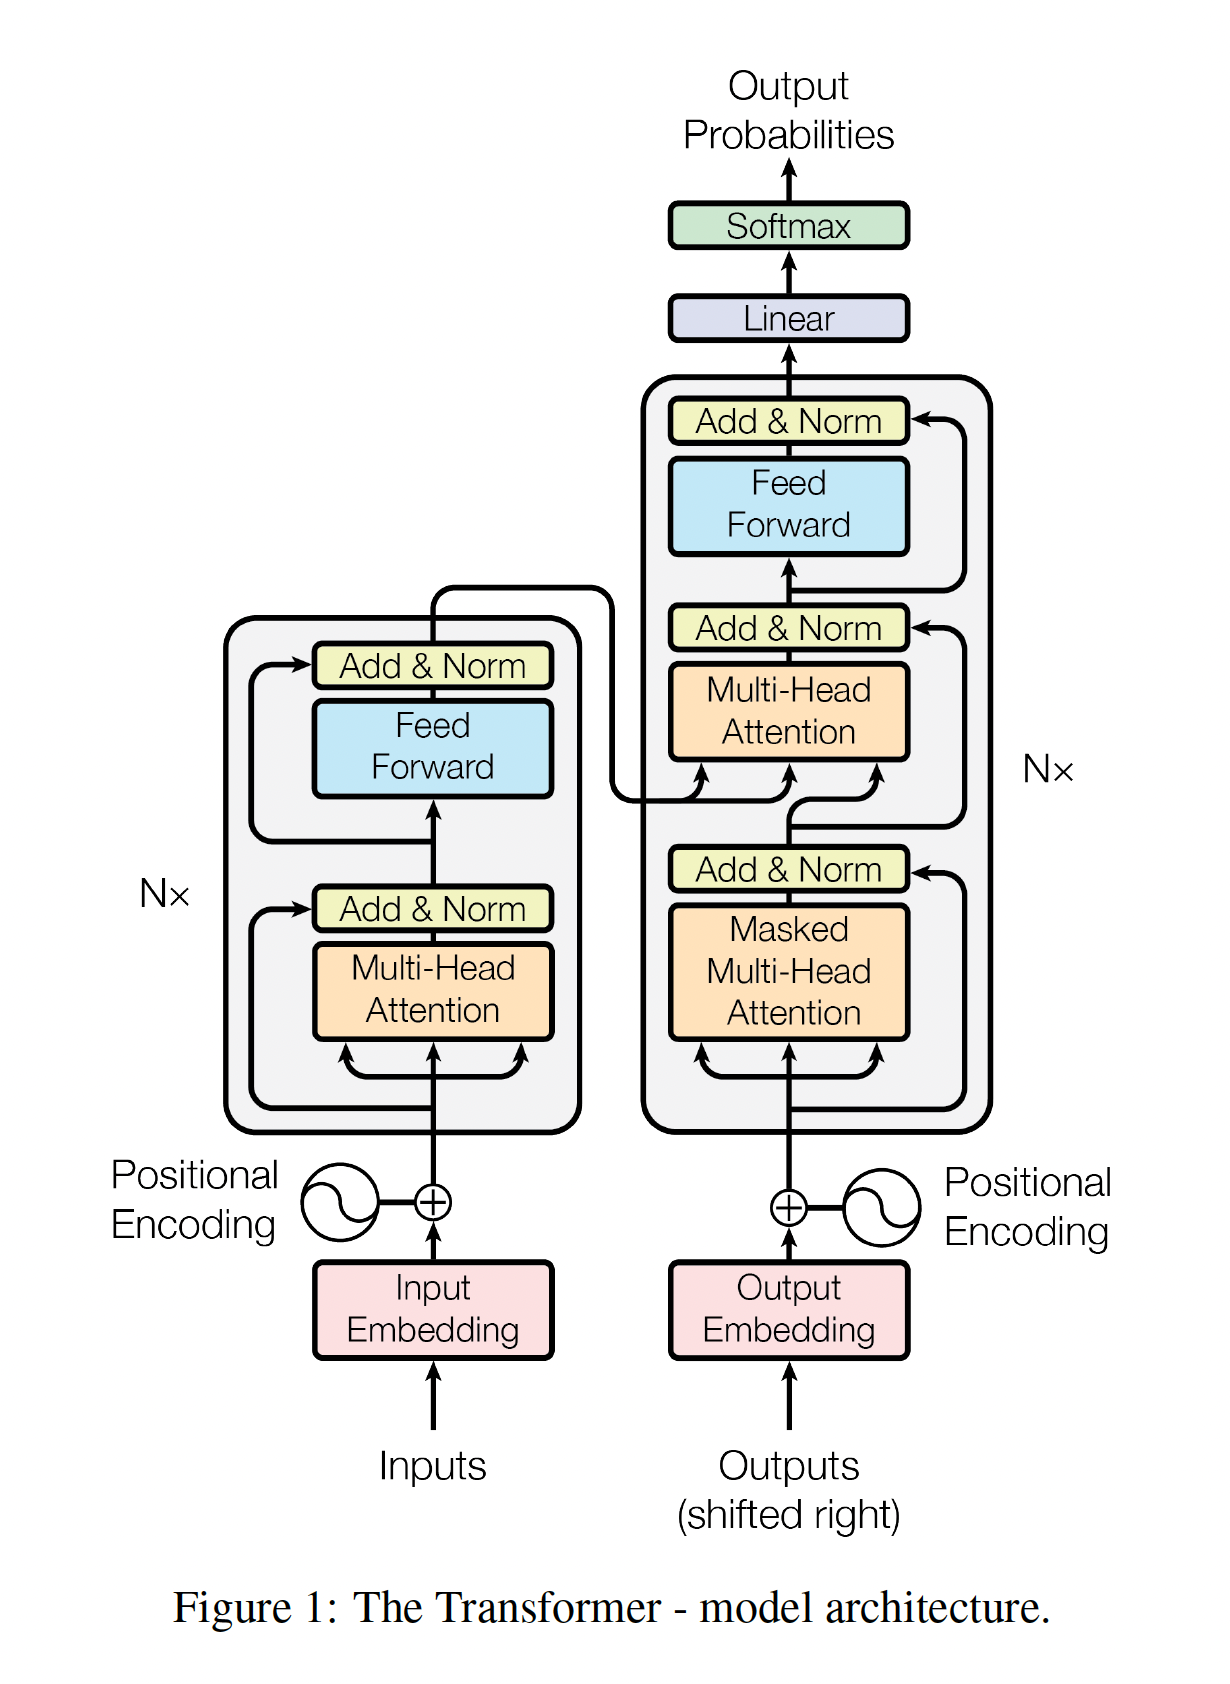
\includegraphics[width=0.55\textwidth]{Assets/transformer_architecture.png}
    \caption{Transformer architecture showing encoder and decoder layers. Source: \cite{vaswani2017attention}}
    \label{fig:transformer_architecture}
\end{figure}

\subsection{Application of LLMs in the World}

Large Language Models (LLMs) have become transformative tools across various domains, showcasing a blend of significant advantages. 

Their applications include enhancing accessibility in education, where they assist in creating personalized learning experiences and automated grading. In legal research, LLMs facilitate efficient document analysis and case summarization. 

Additionally, they improve customer service by powering conversational agents capable of human-like interactions and accelerating drug discovery by enabling advanced analysis of biomedical data. 

Their ability to process, analyze, and generate coherent language makes them invaluable for automating tasks such as summarization, translation, and question-answering~\cite{application_llms}.

\subsubsection{Integration of LLMs in a software engineering project}
Large Language Models (LLMs) have become pivotal tools in software engineering, extending their utility beyond natural language understanding to include code generation, debugging, and automated documentation. Their integration into software engineering projects offers opportunities for streamlining development workflows, improving productivity, and enhancing code quality.

An empirical study conducted by Rasnayaka et al. investigated the impact of LLMs on a semester-long software engineering project involving 214 students \cite{rasnayaka2024}. The findings indicated that LLMs played a significant role in the early stages of development by assisting with foundational tasks such as creating basic design patterns, data structures, and algorithms. A detailed analysis of LLM usage during the project revealed several key insights:
\begin{itemize}
    \item \textbf{Task Distribution:} Prompts generated by students focused on simple tasks (22.95\%), C++ syntax help, and algorithmic solutions (39.34\%).
    \item \textbf{Human Intervention Levels:} The majority of LLM-generated code required minimal modifications, with 19\% of teams accounting for 75\% of all AI-assisted contributions.
    \item \textbf{Phases of Usage:} LLMs were most beneficial in the initial stages of the project, where students relied on them to overcome the steep learning curve of new technologies.
\end{itemize}

Despite their utility, students expressed mixed perceptions. Advanced programmers were more likely to leverage LLMs effectively, while less experienced coders showed hesitance due to challenges in validating AI-generated code for correctness. This underlines the need to integrate LLMs into educational programs thoughtfully, ensuring students develop the necessary foundational skills to collaborate with these tools effectively.

The findings emphasize the importance of adopting a balanced approach, where LLMs are utilized as complementary tools to human creativity and expertise. This ensures that software engineers remain capable of critical thinking and innovation while benefiting from AI's efficiency.
\subsection{Limitations of LLMs}

Despite their potential, LLMs exhibit several limitations that hinder their widespread adoption. One significant concern is their high computational requirements, which strain resources and contribute to environmental costs due to increased energy consumption. 

Furthermore, LLMs are susceptible to biases present in the training data, often resulting in outputs that reinforce stereotypes or inaccuracies. 

They also lack real-world understanding, leading to challenges such as generating misleading or factually incorrect responses. Addressing these issues is vital to ensuring that LLMs become more reliable, equitable, and sustainable for future applications~\cite{limitations_llms}.

Model quantization is a critical technique for reducing the memory footprint and computational cost of large language models (LLMs), enabling their deployment in resource-constrained environments. The study by Lee et al. (2024) evaluates various quantization methods—including GPTQ, AWQ, SmoothQuant, and FP8—on instruction-tuned LLMs ranging from 7B to 405B parameters \cite{lee2024}. Their findings highlight key trade-offs between model size, bit-width, and quantization strategy in preserving model performance across six task types: commonsense reasoning, language understanding, instruction following, hallucination detection, mathematics, and dialogue.

Quantization methods are broadly classified into Post-Training Quantization (PTQ) and Quantization-Aware Training (QAT). While PTQ is widely used due to its efficiency, it may introduce accuracy degradation, particularly in larger models. The study demonstrates that weight-only quantization approaches such as AWQ tend to preserve accuracy better than methods that quantize both weights and activations, especially in LLMs exceeding 405B parameters. Conversely, activation-aware techniques like SmoothQuant struggle to maintain accuracy in high-activation-range models.

Experimental results indicate that larger quantized models often outperform smaller full-precision models across most benchmarks, except in hallucination detection and instruction-following tasks. For instance, a 4-bit quantized Llama-2-13B model surpasses its FP16 Llama-2-7B counterpart despite its smaller storage footprint. Additionally, FP8 quantization, supported by modern hardware like NVIDIA H100 GPUs, provides a stable balance between memory efficiency and computational performance. The study emphasizes that quantization effects depend not only on model architecture but also on dataset complexity and evaluation methodology.

Overall, the findings suggest that careful selection of quantization methods is crucial for maintaining LLM accuracy. Future research should further explore fine-grained trade-offs between precision levels, computational efficiency, and downstream task performance to optimize quantized LLM deployment.

\subsection{Model distillation}
The paper by Gu et al. (2024) presents MiniLLM, an innovative approach to knowledge distillation (KD) designed specifically for large language models (LLMs). Traditional KD methods rely on minimizing the forward Kullback-Leibler (KL) divergence between the teacher and student models, which forces the student to mimic all aspects of the teacher’s output distribution. However, this approach often leads to overestimation of low-probability regions in the teacher model, resulting in poor generalization and exposure bias. To address this issue, the authors propose using reverse KL divergence instead, which encourages the student model to focus on high-confidence regions of the teacher's distribution while avoiding unlikely outputs \cite{gu2024}.

MiniLLM introduces several novel optimization strategies to improve training stability and efficiency. First, the authors employ policy gradient methods to derive a learning objective based on reverse KL minimization. Additionally, they incorporate single-step decomposition to reduce variance, teacher-mixed sampling to prevent reward hacking, and length normalization to ensure balanced text generation. These refinements collectively enable the student model to generate more precise and well-calibrated responses.

Extensive experiments demonstrate that MiniLLM outperforms traditional KD baselines across multiple instruction-following datasets. The method consistently produces student models that generate higher-quality responses with improved calibration and lower exposure bias. Furthermore, MiniLLM scales effectively across different model families, from 120M to 13B parameters, making it a viable solution for compressing large-scale generative models without significant performance degradation.

By focusing on mode-seeking behavior and optimizing training dynamics, MiniLLM offers a scalable and effective approach to distilling large language models. The results suggest that reverse KL-based KD could be a promising direction for future research in efficient model compression and deployment.


\subsection{Most famous companies and models}
The landscape of Large Language Models (LLMs) is dominated by contributions from prominent technology providers, each offering models tailored to various applications. OpenAI's Generative Pre-trained Transformer (GPT) series, including GPT-3, GPT-4, and ChatGPT, stands out for its versatility in tasks such as text generation, summarization, and conversational AI. These models are known for their impressive contextual understanding and human-like responses, supported by fine-tuning through Reinforcement Learning with Human Feedback (RLHF).

Google's BERT (Bidirectional Encoder Representations from Transformers) and its successors, such as LaMDA and PaLM-2, excel in tasks requiring deep contextual embedding, like question answering and natural language understanding. PaLM-2 further pushes the boundaries with enhanced multilingual capabilities and support for multi-modal inputs.

Meta's LLaMA (Large Language Model Meta AI) models, including LLaMA family, are open-source initiatives aimed at democratizing AI research. They emphasize transparency and customization, allowing researchers to fine-tune models for specialized tasks.

Anthropic’s Claude models prioritize safety and interpretability, with a focus on reducing biases and harmful outputs. These models are often used in scenarios requiring ethical AI applications.

In comparison, OpenAI's models generally excel in user-friendly deployment and adaptability, while Google's offerings are stronger in research-focused applications due to their extensive training on multilingual and domain-specific datasets.

Meta’s LLaMA models lead in customization and accessibility for academic research, and Anthropic provides ethical safeguards, making it ideal for sensitive applications.

This diversity highlights the competitive landscape of LLMs, where providers strive to balance performance, safety, and accessibility to meet a wide range of user needs.

\newpage



Abm Agents Expansion
\section{Introduction to Agents and Agent-Based Modelling (ABM)}

Agent-Based Modelling (ABM) is a computational approach for simulating complex systems composed of interacting autonomous agents. Unlike equation-based models, which assume homogeneity and centralized control, ABM focuses on decentralized interactions where each agent operates based on individual rules, behaviors, and decision-making processes \cite{janssen2005}. This paradigm allows for the study of emergent phenomena, where system-level patterns arise from micro-level interactions.

ABM has been widely applied across multiple domains, including economics, ecology, social sciences, and artificial intelligence. It enables researchers to explore how different agents—whether individuals, organizations, or computational entities—adapt, evolve, and interact within dynamic environments. By using ABM as a computational laboratory, various hypotheses related to behavioral rules, decision-making mechanisms, and environmental influences can be systematically tested and refined \cite{janssen2005}.

Moreover, recent advancements in multi-agent systems (MAS) and artificial intelligence have introduced the concept of asynchronous agents, which operate independently and concurrently within a shared environment. Unlike traditional models where agents process events sequentially, asynchronous agents manage multiple concurrent processes in real-time, significantly reducing computational bottlenecks and improving responsiveness \cite{ginart2024}.

\subsection{Short-Term Memory and Asynchronous Processing}

Short-term memory in agents refers to the temporary storage of information that influences immediate decision-making and interactions. In ABM, short-term memory allows agents to retain recent experiences, track environmental changes, and adjust behaviors accordingly. This is particularly useful in dynamic settings where agents must react to fluctuating conditions, such as financial markets or resource allocation problems \cite{janssen2005}.

Incorporating asynchronous processing into short-term memory enhances an agent’s ability to respond to real-time changes. According to \cite{ginart2024}, "giving agents the ability to manage multiple concurrent processes in real-time and asynchronously respond to the user as soon as any process finishes will significantly reduce perceived delay and meaningfully improve user experience." This approach ensures that agents do not remain idle while waiting for new inputs but can instead process multiple stimuli simultaneously, improving adaptability in dynamic systems.

\subsection{Long-Term Memory and Parallel Thought Processes}

Long-term memory in ABM extends beyond immediate reactions, enabling agents to store accumulated experiences and develop complex behavioral strategies over time. Unlike short-term memory, which deals with transient data, long-term memory allows for learning, pattern recognition, and knowledge accumulation.

Recent research on real-time AI agents introduces the concept of parallel thought processes, where agents execute multiple reasoning tasks concurrently rather than sequentially \cite{ginart2024}. This architecture, inspired by concurrent programming, allows agents to "fork" or "spawn" independent sub-processes, each dedicated to a particular task, while maintaining a coherent overarching strategy. For instance, reinforcement learning models within ABM can benefit from parallel execution, optimizing agent decision-making based on asynchronous feedback loops.

\subsection{Multi-Agent Systems and Asynchronous Execution}

A multi-agent system (MAS) consists of multiple interacting agents that collectively influence system dynamics. Unlike single-agent models, MAS emphasizes decentralized control, emergent behaviors, and distributed problem-solving. Agents in MAS may be cooperative, competitive, or a mix of both, depending on the objectives and rules governing interactions.

Traditional MAS often relies on synchronous interactions, where agents follow predefined turn-based sequences. However, as highlighted in \cite{ginart2024}, "current AI systems still operate in a strict turn-based fashion, oblivious to passage of time... forcing user queries and tool-use to occur sequentially, preventing the systems from multitasking and reducing interactivity." Asynchronous execution overcomes these limitations by enabling agents to operate independently, responding to new information without waiting for a complete processing cycle.

\subsection{Multi-Agent Environment and Event-Driven Interaction}

The multi-agent environment refers to the shared space where agents operate, interact, and respond to external stimuli. This environment may be physical (e.g., geographical landscapes in ecological models) or virtual (e.g., cyberspace in AI-driven simulations). The complexity of an environment significantly influences agent decision-making, strategy development, and overall system behavior, requiring adaptive and intelligent coordination mechanisms.

A critical advancement in MAS is the integration of event-driven architectures, which enable more efficient and scalable interaction management. Rather than relying on continuous polling for state updates, agents operate on an event-triggered basis, significantly reducing redundant computations and improving responsiveness. As outlined in \cite{ginart2024}, \textquotedblleft we propose and implement a novel event-driven finite-state machine architecture for executing and prompting AI agents in asynchronous tool environments.\textquotedblright\ This paradigm shift enhances agent efficiency by dynamically allocating computational resources based on event priority rather than rigid scheduling.

Furthermore, event-driven interaction facilitates real-time decision-making and adaptability, allowing agents to respond promptly to changes in the environment. This is particularly beneficial in large-scale multi-agent systems where efficiency and scalability are paramount. By leveraging asynchronous event processing, agents can achieve higher levels of autonomy and robustness, ultimately improving system-wide coordination and collaboration.

\subsection{Adaptive Learning and Self-Optimization in Multi-Agent Systems}

The incorporation of adaptive learning mechanisms into MAS further enhances their capability to operate in complex, dynamic environments. By utilizing reinforcement learning, evolutionary algorithms, or deep learning-based models, agents can refine their strategies over time, improving decision-making and efficiency based on past interactions and environmental feedback.

Self-optimization allows agents to autonomously adjust their operational parameters to maximize performance while minimizing resource consumption. Through techniques such as meta-learning and transfer learning, agents can generalize knowledge across different scenarios, reducing the need for extensive retraining when deployed in new environments.

The combination of event-driven architectures with adaptive learning leads to highly responsive, intelligent multi-agent systems that can continuously evolve. This synergy not only enhances individual agent performance but also strengthens the collective intelligence of the system, making MAS more resilient, scalable, and capable of handling complex real-world applications.

\begin{figure}[H]
    \centering
    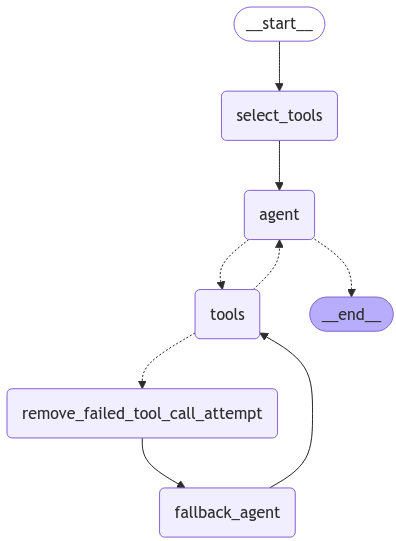
\includegraphics[width=0.5\linewidth]{Assets/complex_agent.png}
    \caption{Exaample of multi agent and multi tool architecure}
    \label{fig:enter-label}
\end{figure}
\subsection{Multi-Agent Interaction and Interrupt Handling}

The interaction between agents is a defining characteristic of ABM, shaping emergent system dynamics. These interactions can be: \begin{itemize} \item \textbf{Direct (Explicit Communication)}: Agents exchange messages, negotiate, or collaborate on tasks. \item \textbf{Indirect (Implicit Influence)}: Agents modify their environment, influencing others without direct communication (e.g., resource depletion in ecological models). \end{itemize}

A key challenge in multi-agent interaction is handling interruptions. Real-time AI agents must be able to prioritize critical updates while continuing background processes. In the architecture proposed by \cite{ginart2024}, agents utilize a "dialog FSM with priority scheduling," ensuring that "interruptions are a first-class feature in an asynchronous agent." This capability mirrors human cognitive flexibility, allowing agents to switch focus dynamically while preserving long-term goals.

\subsection{Agent Use-Cases and Future Directions}

Agent-based modeling has been successfully applied across various disciplines, demonstrating its versatility and analytical power. Some notable use-cases include: \begin{itemize} \item \textbf{Economics}: Studying financial markets, consumer behavior, and macroeconomic trends. \item \textbf{Ecology and Environmental Science}: Understanding land-use patterns, deforestation, and resource conservation strategies. \item \textbf{Social Sciences}: Modeling political polarization and crowd behavior. \item \textbf{Healthcare}: Simulating infectious disease spread and hospital resource allocation. \item \textbf{Artificial Intelligence}: Multi-agent reinforcement learning (MARL) enabling collaborative robotics and adaptive AI agents. \end{itemize}

As ABM continues to evolve, integrating asynchronous execution, real-time decision-making, and event-driven interactions will further enhance its applicability. Future research should explore combining ABM with large action models (LAMs) and instruction-tuned LLMs, as suggested by \cite{ginart2024}, to create truly autonomous, self-improving agent systems.

\subsection{Additional Insights from \cite{ginart2024}}

To expand upon the foundational concepts discussed, we incorporate findings from \cite{ginart2024}. The paper explores additional dimensions of agent-based modeling, particularly in relation to large-scale simulations and real-time agent adaptability. These insights further reinforce the importance of parallel processing, asynchronous execution, and event-driven methodologies in multi-agent environments.

\begin{figure}[h]
\centering
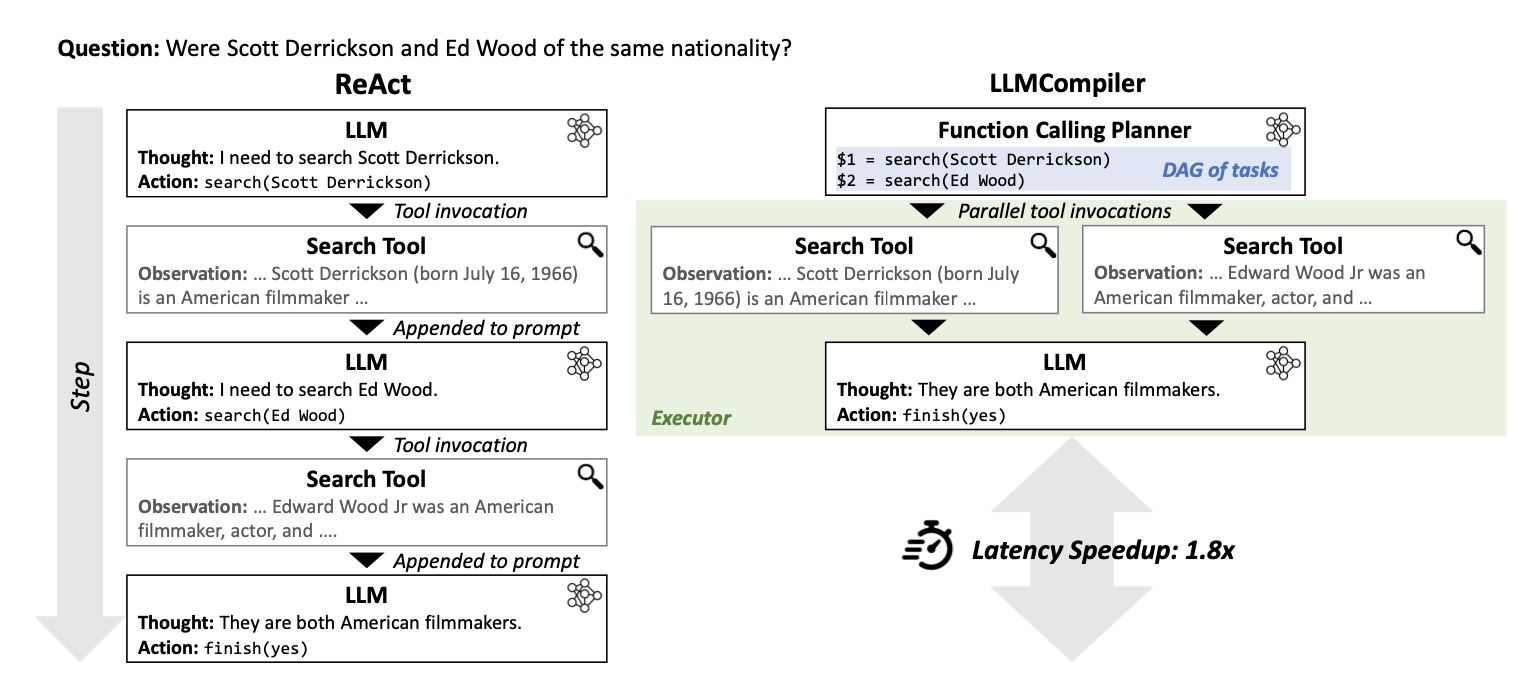
\includegraphics[width=0.8\textwidth]{Assets/agent-architecture.png}
\caption{Comparison between ReAct and LLMCompiler approaches in asynchronous agent execution.}
\end{figure}

\newpage
\subsection{Infrastructure for AI Agents}

As AI agents increasingly operate in open-ended environments, the development of dedicated agent infrastructure becomes crucial. This infrastructure consists of technical systems and shared protocols external to agents, mediating their interactions with the world. According to Chan et al. (2025), agent infrastructure serves three main functions: 
\begin{enumerate}
    \item \textbf{Attribution}—associating actions and properties with specific agents or users.
    \item \textbf{Interaction}—shaping agent interactions with their environment.
    \item \textbf{Response}—detecting and addressing harmful agent actions \cite{chan2025}.
\end{enumerate}

Examples of this infrastructure include:
\begin{itemize}
    \item \textbf{Identity Binding:} Linking agents to legal entities to ensure accountability.
    \item \textbf{Agent IDs:} Unique identifiers for tracking and managing agent activities.
    \item \textbf{Oversight Layers:} Mechanisms for monitoring and intervening in agent behavior.
    \item \textbf{Commitment Devices:} Ensuring agents adhere to predefined actions or rules.
\end{itemize}

This approach not only facilitates accountability and trust but also addresses potential risks associated with the deployment of advanced agents, such as security vulnerabilities or unintended actions. Future directions in ABM could include exploring how this infrastructure can integrate with multi-agent systems and enable large-scale, cooperative simulations in diverse applications.



\listoffigures
\listoftables


\bibliographystyle{siam}

\begin{thebibliography}{1}
\bibitem{1} Glez-Peña, Daniel, et al. "Web scraping technologies in an API world." Briefings in Bioinformatics 15.5 (2014): 788-797.

\bibitem{lee2024} 
J. Lee, S. Park, J. Kwon, J. Oh, and Y. Kwon, 
\textit{A Comprehensive Evaluation of Quantized Instruction-Tuned Large Language Models: An Experimental Analysis up to 405B}, 
arXiv preprint arXiv:2409.11055, 2024.

\bibitem{hirsch2014} 
Dennis D. Hirsch, ``The Glass House Effect: Big Data, the New Oil, and the Power of Analogy,'' \textit{Maine Law Review}, vol. 66, no. 2, 2014, pp. 373-396.

\bibitem{decker1997}
K. Decker, K. Sycara, and M. Williamson. Middle-agents for the Internet. In *Proceedings of the Fifteenth International Joint Conference on Artificial Intelligence (IJCAI)*, 1997.

\bibitem{abar2017}
    S. Abar, G. K. Theodoropoulos, P. Lemarinier, and G. M. P. O’Hare, ``Agent Based Modelling and Simulation tools: A review of the state-of-art software,'' \emph{Computer Science Review}, vol. 24, pp. 13–33, 2017.

\bibitem{azad2020} Azad, Babak Amin, et al. "Web Runner 2049: Evaluating Third-Party Anti-bot Services." \textit{DIMVA 2020, Lecture Notes in Computer Science}, vol. 12223, 2020, pp. 135–159. Springer, https://doi.org/10.1007/978-3-030-52683-2\_7.

\bibitem{schelen1998qosagents}
O. Schelén, \emph{Quality of Service Agents in the Internet}, Doctoral Thesis, Department of Computer Science and Electrical Engineering, Luleå University of Technology, 1998.

\bibitem{darmawan2022evaluating}
I. Darmawan, M. Maulana, R. Gunawan, and N. Widiyasono, ``Evaluating Web Scraping Performance Using XPath, CSS Selector, Regular Expression, and HTML DOM With Multiprocessing,'' \emph{International Journal on Informatics Visualization}, vol. 6, no. 4, pp. 904-910, 2022.

\bibitem{David2008}
P.~A. David and J.~S. Shapiro, ``Community-based production of open-source software: What do we know about the developers who participate?'' \emph{Information Economics and Policy}, vol.~20, no.~3, pp. 364–398, 2008.

  \bibitem{ahluwalia2023}
    A. Ahluwalia and S. Wani, ``Leveraging Large Language Models for Web Scraping,'' \emph{arXiv preprint arXiv:2406.08246v1}, 2023.
\bibitem{vaswani2017attention}
A. Vaswani, N. Shazeer, N. Parmar, J. Uszkoreit, L. Jones, A. N. Gomez, Ł. Kaiser, and I. Polosukhin, ``Attention is All You Need,'' \textit{Advances in Neural Information Processing Systems (NeurIPS)}, pp. 5998--6008, 2017.
 \bibitem{application_llms} Hadi, M. U., Tashi, Q. A., Shah, A., et al., "Large Language Models: A Comprehensive Survey of its Applications, Challenges, Limitations, and Future Prospects," TechRxiv, 2024

\bibitem{rasnayaka2024}
Rasnayaka, S., Wang, G., Shariffdeen, R., \& Iyer, G. N. (2024). An Empirical Study on Usage and Perceptions of LLMs in a Software Engineering Project. \textit{Proceedings of the 2024 International Workshop on Large Language Models for Code (LLM4Code ’24)}, April 20, Lisbon, Portugal. ACM, New York, NY, USA \url{https://doi.org/10.1145/3643795.3648379}.
\bibitem{limitations_llms} Hadi, M. U., Tashi, Q. A., Shah, A., et al., "Large Language Models: A Comprehensive Survey of its Applications, Challenges, Limitations, and Future Prospects," TechRxiv, 2024.

\bibitem{janssen2005} Janssen, M. A. (2005). Agent-Based Modelling. \textit{Internet Encyclopaedia of Ecological Economics}, Arizona State University.

\bibitem{janssen2005} Janssen, M. A., \& Ostrom, E. (2005). Empirically based, agent-based models. Ecology and Society, 10(2), 37.



\bibitem{ginart2024} Ginart, A. A., Kodali, N., Lee, J., Xiong, C., Savarese, S., \& Emmons, J. (2024). Asynchronous Tool Usage for Real-Time Agents. Salesforce AI Research.



\bibitem{ginart2024} Ginart, A., et al. (2024). Asynchronous Agents in Real-Time AI Systems. arXiv preprint arXiv:2312.04511.

\bibitem{chan2025}
A. Chan, K. Wei, S. Huang, N. Rajkumar, E. Perrier, S. Lazar, G. K. Hadfield, and M. Anderljung.
\newblock Infrastructure for AI Agents.
\newblock \emph{arXiv preprint arXiv:2501.10114}, 2025.

\bibitem{bigdatawire2024}
Big Data Wire. (2024, March 6). \textit{GenAI doesn’t need bigger LLMs, it needs better data}. \url{https://www.bigdatawire.com/2024/03/06/genai-doesnt-need-bigger-llms-it-needs-better-data/}

\bibitem{privacyos2024}
PrivacyOS. (2024). \textit{The 95\% of sanctions is triggered by an offense on personal data and consents}. \url{https://www.privacyos.com/en/the-95-of-sanctions-is-triggered-by-an-offense-on-personal-data-and-consents/}

\bibitem{webscraper2024}
WebScraper. A brief history of web scraping. Retrieved November 5, 2024, from \url{https://webscraper.io/blog/brief-history-of-web-scraping}

\bibitem{humby2006}
Humby, C. (2006). *Data is the new oil. It's valuable, but if unrefined it cannot really be used. It has to be changed into gas, and gasoline is used to power a car.*

\bibitem{McCulloch1943}
Warren S. McCulloch and Walter Pitts, 
"A logical calculus of the ideas immanent in nervous activity," 
\textit{The Bulletin of Mathematical Biophysics}, 
vol. 5, no. 4, pp. 115--133, Dec. 1943. 
DOI: \href{https://doi.org/10.1007/bf02478259}{10.1007/bf02478259}.

\bibitem{glez-pena2013} 
Daniel Glez-Peña, Ana Lourenço, Hugo López-Fernández, Miguel Reboiro-Jato, and Florentino Fdez-Riverola. 
\textit{Web scraping technologies in an API world}. Briefings in Bioinformatics, Vol. 15, No. 5, 788-797, 2013.

\bibitem{citeseerx2024}
CiteSeerX. (2024). \textit{The Growing Value of Private Data}. \url{https://citeseerx.ist.psu.edu/document?repid=rep1&type=pdf&doi=e4ae9f8b13fab5c5ce1e1e820b64bce196f60c53}

\bibitem{runacap2024}
Runacap's Ross Index. \emph{Q3 2024 Report on Fastest-Growing Open-Source Libraries}, 2024. \url{https://runacap.com/ross-index/q3-2024/}.


\bibitem{Morris1999} 
R.G.M. Morris, ``D.O. Hebb: The Organization of Behavior, Wiley: New York; 1949,'' \textit{Brain Research Bulletin}, vol. 50, no. 5-6, p. 437, Nov. 1999, doi: \href{https://doi.org/10.1016/s0361-9230(99)00182-3}{10.1016/s0361-9230(99)00182-3}.

\bibitem{LSTM}
S. Hochreiter and J. Schmidhuber, ``Long Short-term Memory,'' \textit{Neural Computation}, vol. 9, pp. 1735-80, Dec. 1997, doi: \href{https://doi.org/10.1162/neco.1997.9.8.1735}{10.1162/neco.1997.9.8.1735}.



   .
    
\bibitem{shreekumar2022importance}
Shreekumar, S., Mundke, S., \& Dhanawade, M. (2022). \textit{Importance of Web Scraping in E-Commerce Business}. NCRD’s Technical Review: e-Journal, 7(1). Sterling Institute of Management Studies.

 \bibitem{jiang2023}
    Z. Jiang, F. F. Xu, L. Gao, Z. Sun, Q. Liu, J. Dwivedi-Yu, Y. Yang, J. Callan, and G. Neubig, ``Active Retrieval Augmented Generation,'' \emph{arXiv preprint arXiv:2305.06983v2}, 2023.
\bibitem{hadi2024}
Hadi, M. U., Al Tashi, Q., Shah, A., et al. (2024). Large Language Models: A Comprehensive Survey of Its Applications, Challenges, Limitations, and Future Prospects. \textit{TechRxiv Preprints}. Retrieved from \url{https://doi.org/10.36227/techrxiv.23589741.v6}.

\bibitem{Tamburri2019}
D.~A. Tamburri, F.~Palomba, A.~Serebrenik, and A.~Zaidman, ``Discovering community patterns in open-source: A systematic approach and its evaluation,'' \emph{Empirical Software Engineering}, vol.~24, no.~3, pp. 1369–1417, 2019.


\end{thebibliography}

\chapter{Benchmarks and comparisons}

The development and deployment of data extraction techniques require thorough evaluation to ensure their effectiveness, scalability, and practicality. This chapter focuses on the benchmarks and comparisons of various methods used for extracting data, emphasizing the transformative role of large language models (LLMs) in this domain.

Traditional data extraction tools have relied on rule-based approaches or simpler frameworks, which often struggle to adapt to complex, dynamic data sources. The emergence of LLMs has provided a new paradigm, enabling advanced capabilities for processing unstructured and long-context data. These models not only enhance data extraction precision but also significantly reduce the complexity of integrating and utilizing diverse data sources.

In this chapter, we analyze the effectiveness of LLMs for data extraction in two critical contexts: internet-based data and private documents. The internet context examines the importance of publicly available data in AI development, highlighting the challenges of quality versus scale in data collection. Meanwhile, the document context addresses the pressing need to extract information from private data repositories securely and ethically, especially as they represent the majority of the world's data.

Furthermore, this chapter outlines the architecture and integration of the ScrapegraphAI library, emphasizing its modular and scalable design. By leveraging distinct nodes for specialized tasks, such as fetching, parsing, and searching, the library ensures adaptability and efficiency in handling complex data workflows. Through a comprehensive evaluation of these approaches, we aim to provide insights into their performance and potential improvements, contributing to the future of scalable and responsible data extraction solutions.
\section{Use of LLMs for extracting data}
It is estimated that $95\%$ of the world's data is not publicly available and is instead private, while only $5\%$ can be sourced from the internet and public sources. As a result, there is a significant gap in the ability to analyze this private data, as no existing library or framework currently provides this capability. This has led to a growing demand for document and PDF scraping tools. Furthermore, the use of Large Language Models (LLMs) is necessary for extracting information from lengthy and complex files.

\subsection{Internet context}
The exponential growth of artificial intelligence (AI) applications in recent years has highlighted the critical importance of data as a foundation for building and improving AI systems. Prior to the advent of large language models (LLMs), data sourced from the internet already played a fundamental role in AI development. Web data—such as social media interactions, forum discussions, news articles, and online marketplaces—provided an accessible and diverse resource that allowed early AI models to learn from a wide range of human activities and patterns.

This internet-sourced data was crucial in areas like sentiment analysis, recommendation systems, and image recognition, where models benefited from observing and categorizing large volumes of unstructured, real-world information. Market research data, for example, offered valuable insights into consumer behavior and preferences, supporting businesses in making data-driven decisions and personalizing their offerings to customers. By leveraging these vast data sources, AI researchers could train models to perform specific tasks based on the patterns and nuances present in this collected information.

However, as the field advanced and LLMs became more prominent, the focus shifted towards scaling model parameters to achieve more sophisticated language and vision capabilities. While large datasets remained necessary, contemporary research and industry practices increasingly recognize that enhancing the quality of data can have a more significant impact on model performance than simply increasing model size \cite{bigdatawire2024}. Indiscriminately collected datasets often introduce noise, redundancy, or irrelevant information, which may hinder a model’s accuracy and effectiveness.

High-quality data—characterized by accuracy, relevance, and minimal noise—empowers AI systems to make more precise predictions and reduces the computational resources required for training and deploying large-scale models. Consequently, the future of AI development is moving toward curating targeted, high-quality data sources rather than relying solely on large-scale, generalized data scraped from the internet. 

This approach prioritizes data quality, balancing computational efficiency with enhanced model reliability and specificity in diverse AI applications.


\begin{figure} [H]
    \centering
    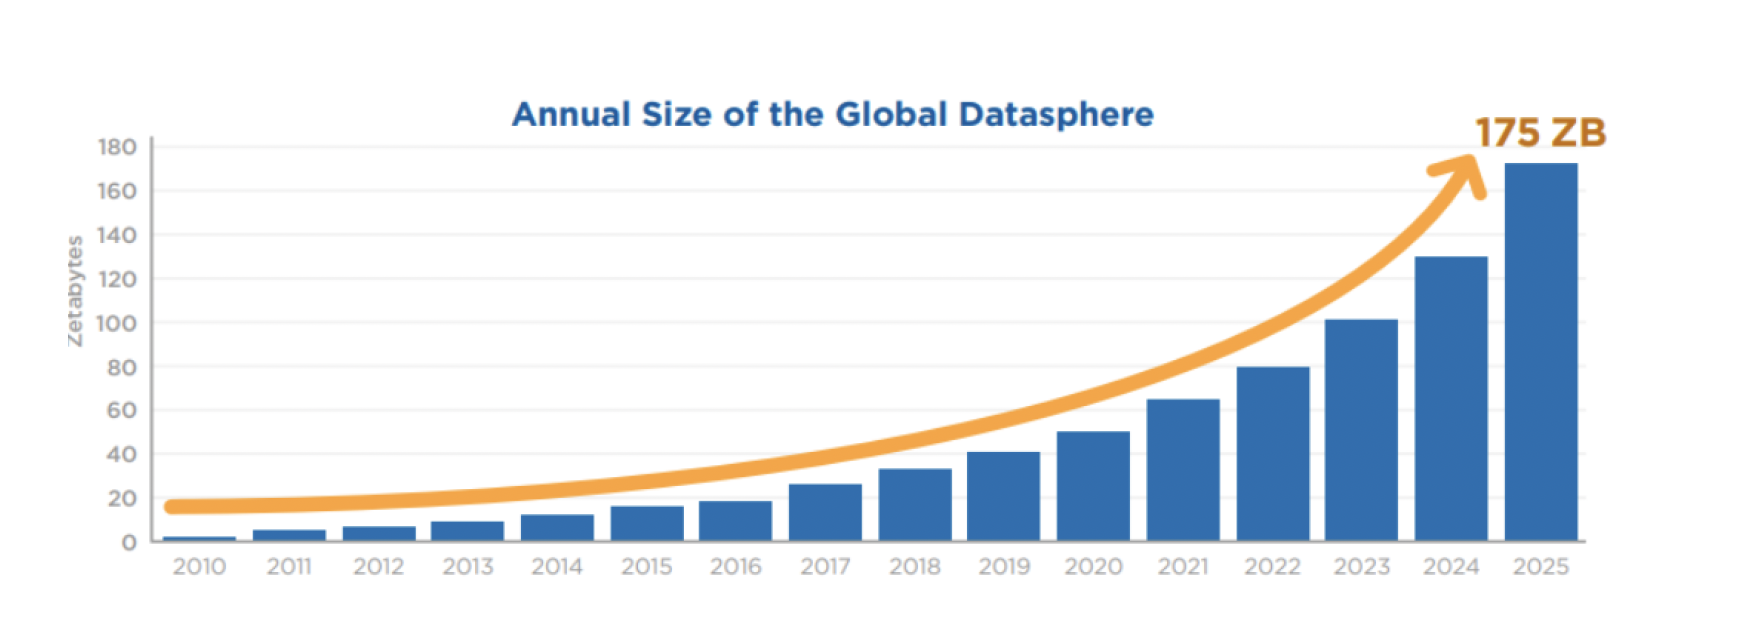
\includegraphics[width=0.95\linewidth]{Assets/required_data.png}
    \caption{Produced data forecasting, source: International Data Companion (IDC)}
    \label{fig:enter-label}
\end{figure}
\subsection{Documents context}
The importance of private documents and the data they contain cannot be overstated, especially considering that approximately 95\% of global data is not publicly accessible on the internet. This significant portion of data, often found in private documents, proprietary research, and organizational databases, holds immense potential for enhancing the capabilities of AI systems. 

By integrating insights from these resources, AI can achieve a more comprehensive understanding of complex phenomena, particularly in specialized fields such as healthcare, finance, and legal affairs. For example, private medical records can provide critical data for training AI models aimed at improving diagnostics and personalized treatment plans, while financial records can enhance predictive analytics in market trends.

However, the challenge of accessing and utilizing this private data is compounded by issues related to privacy, consent, and data protection. 

A staggering 95\% of sanctions for data breaches arise from offenses concerning personal data and inadequate consent management \cite{privacyos2024}. This reality highlights the necessity for organizations to implement stringent data governance policies and comply with regulations such as the General Data Protection Regulation (GDPR) in Europe. These regulations demand meticulous handling of personal information, ensuring that individuals' rights are protected while enabling responsible data use.

To unlock the value of private documents for AI development, a balanced approach is needed that prioritizes both data utility and compliance with privacy standards. Developing frameworks for securely managing and anonymizing sensitive data could facilitate safer access to these valuable information sources. By fostering an environment where private data can be ethically utilized, organizations can not only enhance AI capabilities but also build public trust and align their practices with responsible data management principles. This strategic emphasis on high-quality, ethically sourced data is crucial for driving the future of AI in a direction that respects individual privacy while harnessing the power of information.
\newpage

\section{Structure of the library}
\subsection{Basic integration}

From the beginning the idea was to have a modular framework that enables to change least number of lines of code for having a working script. 

All this leads to a very fast learning curve of the library that allows you not to know the HTML code and CSS selectors and consequently to a time saving.

As it is possible to see from the figure \ref{fig:scrapegraph-script} it is just needed to change the prompt and the source lines of code for making work the extraction pipeline. First you need to choose a provider from those available.

\begin{figure}[H]
    \centering
    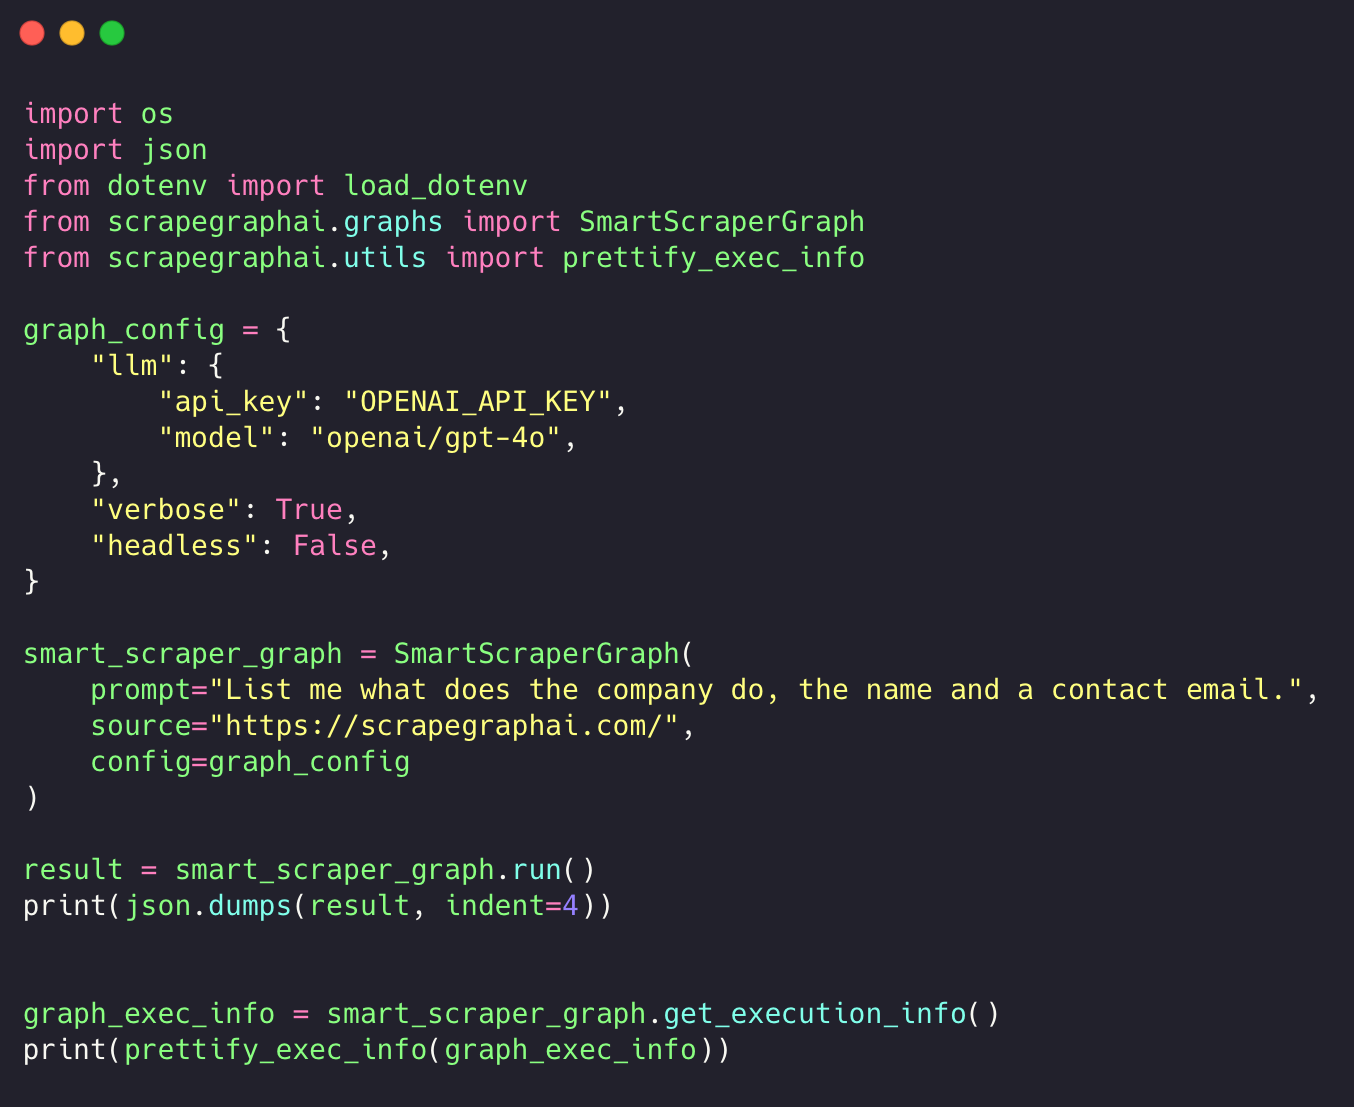
\includegraphics[width=0.75\linewidth]{Assets/scrapegraph_integration.png}
    \caption{Basic integration of ScrapegraphAI }
    \label{fig:scrapegraph-script}
\end{figure}

\subsection{Framework introduction}

In the context of the ScrapegraphAI  library, a node represents a fundamental unit designed to execute a distinct action. Each node contributes to the overall workflow by performing a well-defined function, maintaining a high degree of modularity and atomization. This modular approach ensures that each component or module is responsible for a unique and specific task.

These tasks range broadly from retrieving data from the internet to formulating responses through the integration of large language models (LLMs). It is important to note, however, that not all modules leverage generative AI; some perform other specialized operations to support the broader system functionalities. This architectural choice promotes scalability, adaptability, and ease of maintenance within the ScrapegraphAI  framework.
\subsection{Principal nodes}
This chapter will discuss the principal nodes of the library. 
\subsubsection{Fetch\_node}
It's the node in charge for loading the documents to the state's dictionary.

It can fetch informations for whatever whitch documetn avaiable, example of formats are: JSON, XML, CSV, MD, HTML and PDF.

Regarding the download of the informations from the internet it uses a ChromiumLoader istance. It could be headless or not.

It is possible  also to fetch the code with external headless providers like Browserbase and Scrape.do.

\subsubsection{Fetch\_node\_level\_k}
Fetch\_node\_level\_k is a node responsible for fetching the HTML content of a specified URL and all its sub-links recursively up to a certain level of hyperlink depth. This content is then used to update the graph's state. It uses ChromiumLoader to fetch the content from a web page asynchronously (with proxy protection).

\subsubsection{Parse\_node}
It parses the HTML code to markdown because the LLM can understand better the context rather than the first one.

\subsubsection{Search\_internet\_node}
It allows to make searches in the internet for finding links given a query as input..

\subsubsection{Generate\_answer\_node}
This is the key node of the library. It uses an LLM for generating answers given a prompt, the parsed text of the website and an optional output schema.

There are many variants of this node depending on the type of graph you want to use.

\subsubsection{Generate\_answer\_node\_k\_level}
Generate\_answer\_node\_k\_level is a node responsible for compressing the input tokens and storing the document in a vector database for retrieval. Relevant chunks are stored in the state. It allows scraping of big documents without exceeding the token limit of the language model.

\subsubsection{Html\_analyzer\_node}
The Html\_analyzer\_node module analyzes HTML code based on the desired information to be extracted and returns a reduced version of the HTML content. The output of this node is primarily intended to enhance the reasoning capabilities of the GenerateCodeNode, enabling it to generate more accurate and context-aware code.

\subsubsection{Conditional\_node}
It represent an if-else condition in the generation of the graphs. It is used when a condition in the state could be respected or not.

\subsubsection{Description\_node}
Description\_node is a node responsible for compressing the input tokens and storing the document in a vector database for retrieval. Relevant chunks are stored in the state. It allows scraping of big documents without exceeding the token limit of the language model.

\subsection{Principal graphs}

This section will discuss the principal graphs of the library
\subsubsection{Smart\_scraper}
The SmartScraperGraph is the most used pipeline and is made by three components.
\begin{itemize}
    \item \textbf{FetchNode}: allows to fetching the source code from the target website
    \item \textbf{ParseNode}: it parse the HTML code to markdown-style format
    \item \textbf{GenerateAnswerNode}: it uses an llm provider for generating the asnwer according to the task and the optional task
\end{itemize}
\begin{figure}[H]
    \centering
    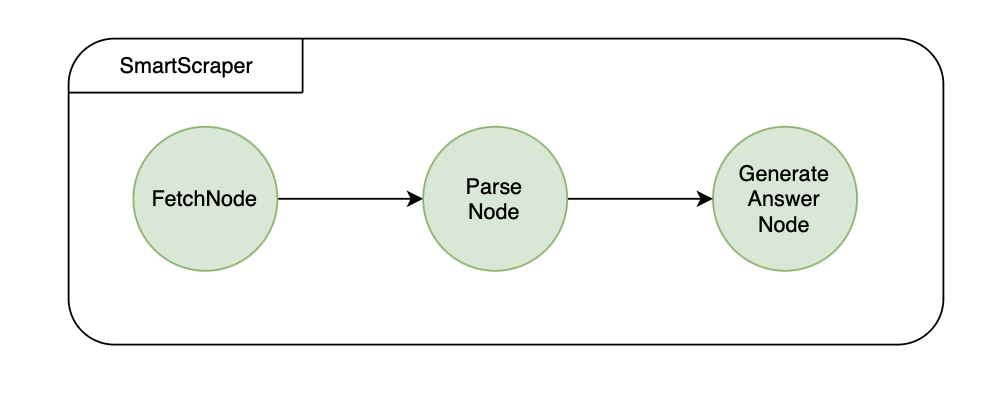
\includegraphics[width=0.75\linewidth]{Assets/smart_scraper.png}
    \caption{Smart\_scraper}
    \label{fig:smart_scraper}
\end{figure}

\subsubsection{Smart\_scraper\_lite\_graph}
It's a ligthweigth version of the smart\_scraper\_graph where it uses just three nodes instead of two.

The submodules inside this graph are:

\begin{itemize}
    \item \textbf{FetchNode}: for fetching the code
    \item \textbf{GenerateAnswerNode}: for generating the asnwer
\end{itemize}

\begin{figure}[H]
    \centering
    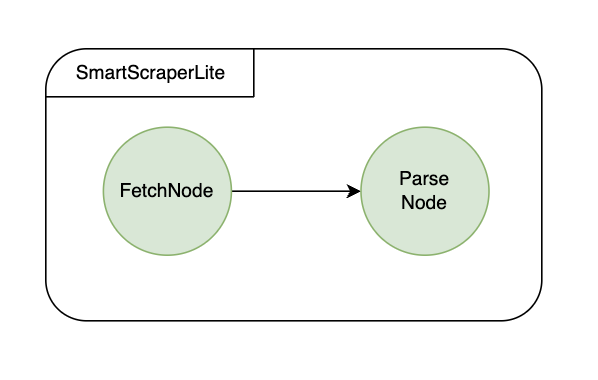
\includegraphics[width=0.5\linewidth]{Assets/smart_scraper_lite.png}
    \caption{Smart\_scraper\_lite}
    \label{fig:enter-label}
\end{figure}
\subsubsection{Search\_graph}
The search\_graph is an example of graph that embeds another graph inside it.

The input of this pipeline is just a query to search on internet and an optional schema and it returns a json file as output .

The peculiarity of this is, starting from the beginning the SearchInternetNode which allows to search on internet the links of the given the query and it return a certain number of links specified by the user.

After this phase the GraphIteratorNode invokes n istances of the SmartScraperGraph where n is the number of links returned by the previous node.
\begin{figure}[H]
    \centering
    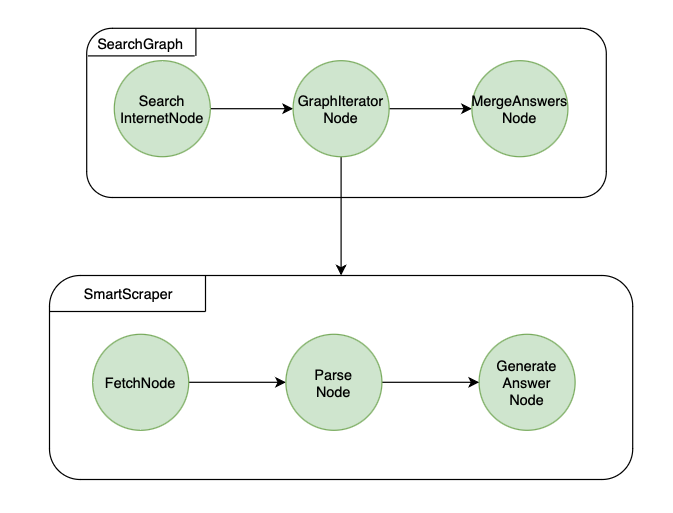
\includegraphics[width=1\linewidth]{Assets/search_graph.png}
    \caption{Search\_graph}
    \label{fig:enter-label}
\end{figure}
\subsubsection{JSON\_scraper}
It's the graph in charge of extracting data from JSON's files.

The modules of this graph are: 
\begin{itemize}
    \item \textbf{FetchNode}: for loading in the state the JSON document 
    \item \textbf{GeneateAnswerJsonNode}: for generating the answer 
\end{itemize}

\begin{figure}[H]
    \centering
    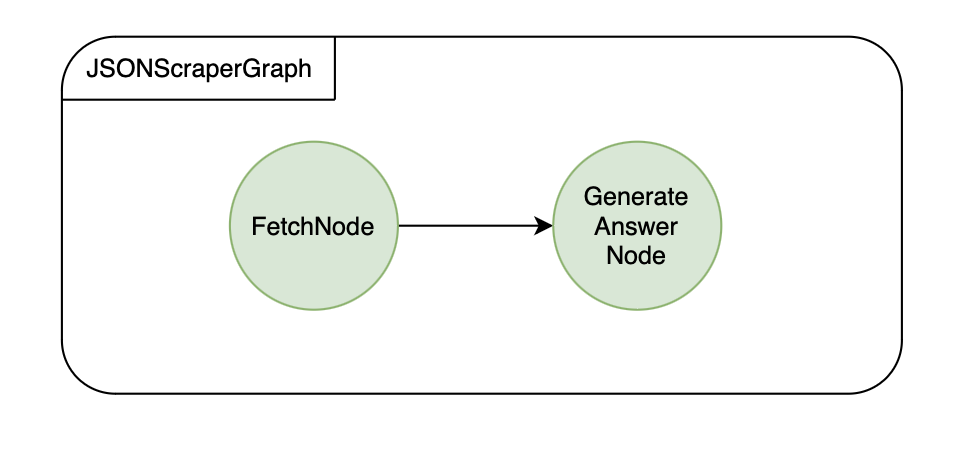
\includegraphics[width=0.75\linewidth]{Assets/json_scraper.png}
    \caption{JSON\_scraper}
    \label{fig:json_scraper}
\end{figure}
\subsubsection{CSV\_scraper}
It's the graph in charge of extracting data from CSV's files.

The modules of this graph are: 
\begin{itemize}
    \item \textbf{FetchNode}: for loading the informations from a CSV document to the state.
    \item \textbf{GeneateAnswerCSVNode}: for creating a structured answer.
\end{itemize}

\begin{figure}[H]
    \centering
    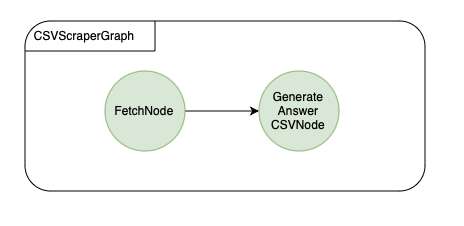
\includegraphics[width=0.75\linewidth]{Assets/csv_scraper.png}
    \caption{CSV\_scraper}
    \label{fig:csv-scraper}
\end{figure}
\subsection{Multiple request and parallelism integration}
As regards the management of multiple requests, ad hoc pipelines have been created to manage parallelism.

To manage this challenge, the graph called SmartScraperMultiGraph was created.
As you can see from the image \ref{fig:multi}, it is very similar to SerchGraph but it does not search Google from queries.
The core remains the GraphIteratoNode that allows you to iterate the many instances of SmartScraper.
\begin{figure}[H]
    \centering
    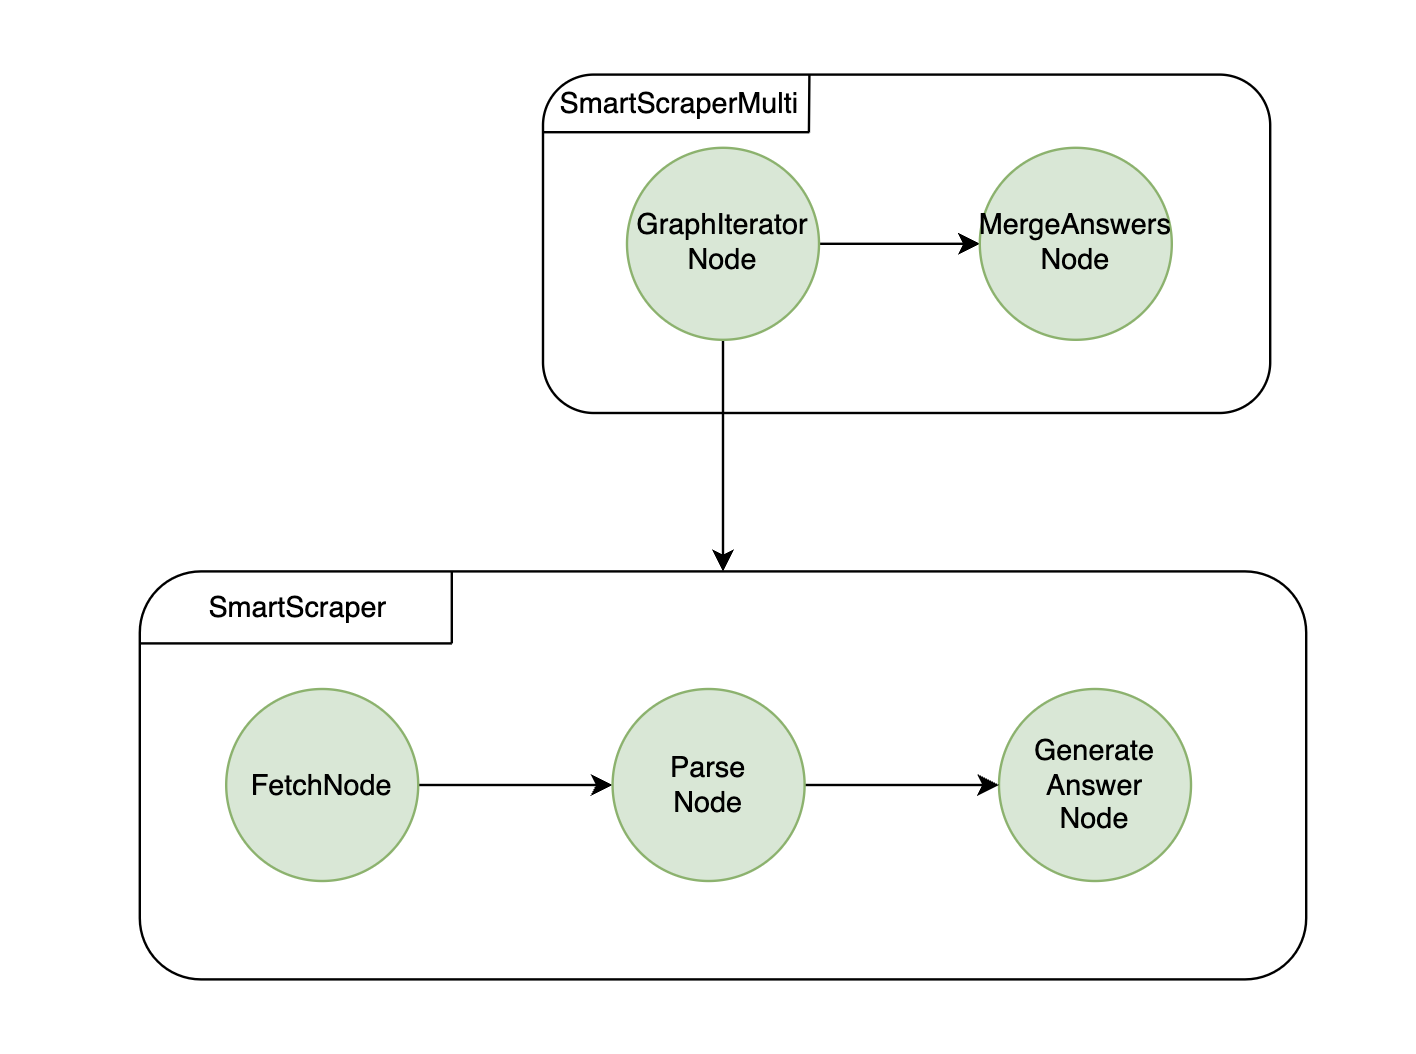
\includegraphics[width=0.75\linewidth]{Assets/multi_graph.png}
    \caption{Parallelism integration for SmartScraperGraph}
    \label{fig:multi}
\end{figure}


\subsection{Output schema integration}
From version 0.26.1 onward, ScrapegraphAI allows the use of a Pydantic schema to specify the desired output format. This is a crucial feature in the context of large-scale web scraping, as it directly addresses several challenges related to data consistency, validation, and scalability.

One of the most critical challenges in web scraping, particularly when dealing with large-scale operations, is ensuring that the extracted data remains consistent and usable, regardless of the diverse sources from which it originates. Web data is inherently heterogeneous, with websites differing significantly in how they structure and present information. This variability can lead to inconsistencies in the scraped data, such as missing fields, incorrect data types, or improperly formatted information. If left unchecked, these inconsistencies can disrupt downstream processing and analysis, potentially leading to incorrect conclusions or failure in automated systems.

In the case of ScrapeGraph, where data is not only extracted but also structured into a graph-based format, these inconsistencies can compromise the quality of the entire system. Graphs depend on a standardized structure to link data from various nodes (websites) effectively, and without a clear output schema, the process of generating and linking nodes becomes error-prone and inefficient.

The introduction of a well-defined output schema addresses these challenges by imposing a structured format on the scraped data. An output schema acts as a framework that ensures all extracted data follows a uniform structure, making it easier to validate, process, and store. This consistency across datasets is essential for several reasons:

\begin{itemize}
    \item \textbf{Error Detection}: A schema simplifies error detection by defining expected data types, fields, and relationships. It allows the system to easily spot anomalies or missing data, enabling faster identification of issues and more effective troubleshooting.
    \item \textbf{Scalability}: With a standardized schema, ScrapegraphAI can easily scale to handle new scraping tasks. As the system can rely on a uniform output format, integrating new data sources requires minimal adjustments. This reduces the complexity of adding new websites to the scraping pipeline.
    \item \textbf{Data Integration and Linking}: A consistent output schema facilitates the integration of scraped data into a unified graph. The schema ensures that data from different sources can be linked and structured effectively, a core requirement for building the interconnected data graph that ScrapegraphAI aims to generate. This makes it possible to aggregate and analyze data from multiple sources in a cohesive manner.
\end{itemize}

In addition, by using Pydantic schemas, ScrapegraphAI ensures that the output data adheres to predefined models, which can also enforce data validation and provide automatic type checking. This integration enhances the robustness of the scraping process, allowing for more reliable and efficient data extraction.

\begin{figure}[H]
    \centering
    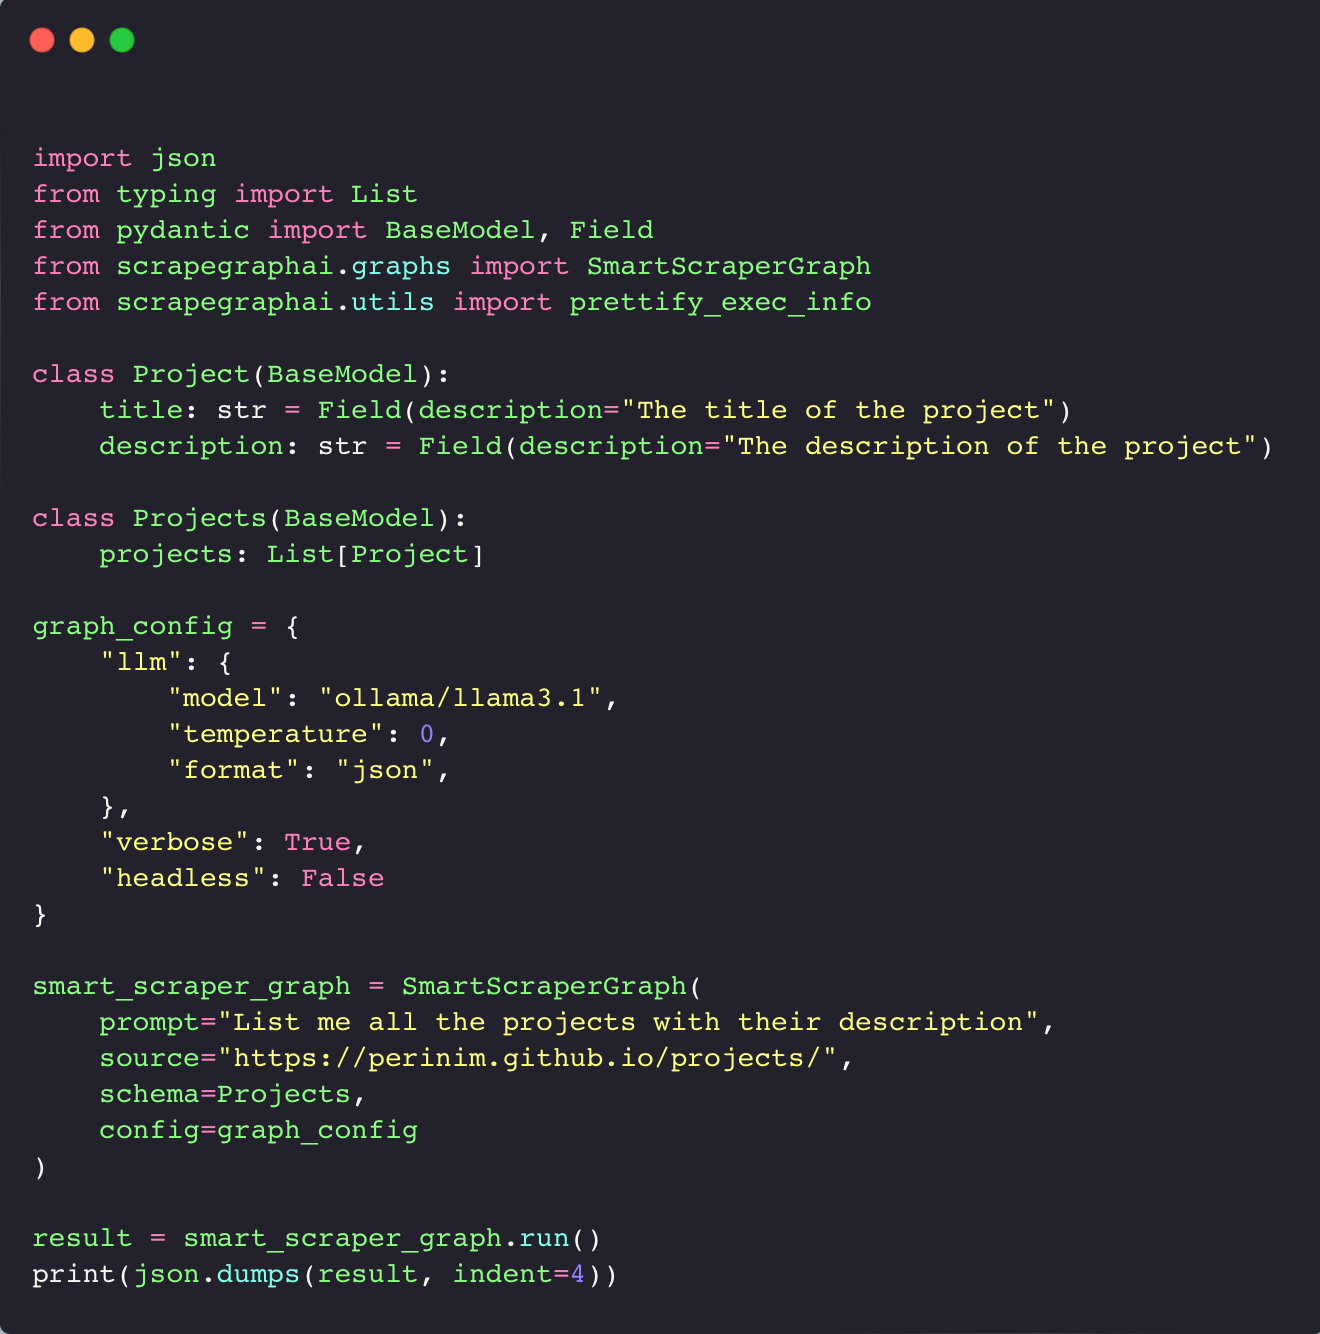
\includegraphics[width=1\linewidth]{Assets/schema_integration.png}
    \caption{Example of schema integration with Pydantic}
    \label{fig:enter-label}
\end{figure}


\subsection{A new paradigm an LLM that generates code for scraping}
One of the most interesting approaches of this library is not so much the creation of scripts that as output lead to the creation of structured outputs, but rather scripts that as output create scripts in Beautifoulsoup or Scrapy.
The consequence that can have is the reduction of costs in classic scraping pipelines, where for example instead of calling a technician who fixes the scripts you can use one of the two classes of graphs that are described in the two following sections that write the new code.

The operation of this category of scripts is described in the figure \ref{fig:actually indians}.

As is it possible to see from it, you can notice that it allows you to avoid using real people within the process, leading to a reduction in costs for the company and at the same time it is less expensive than the classic ScrapegraphAI  classes because it uses the LLMs only to generate the new scraping scripts instead of using them every time.

\begin{figure}[H]
    \centering
    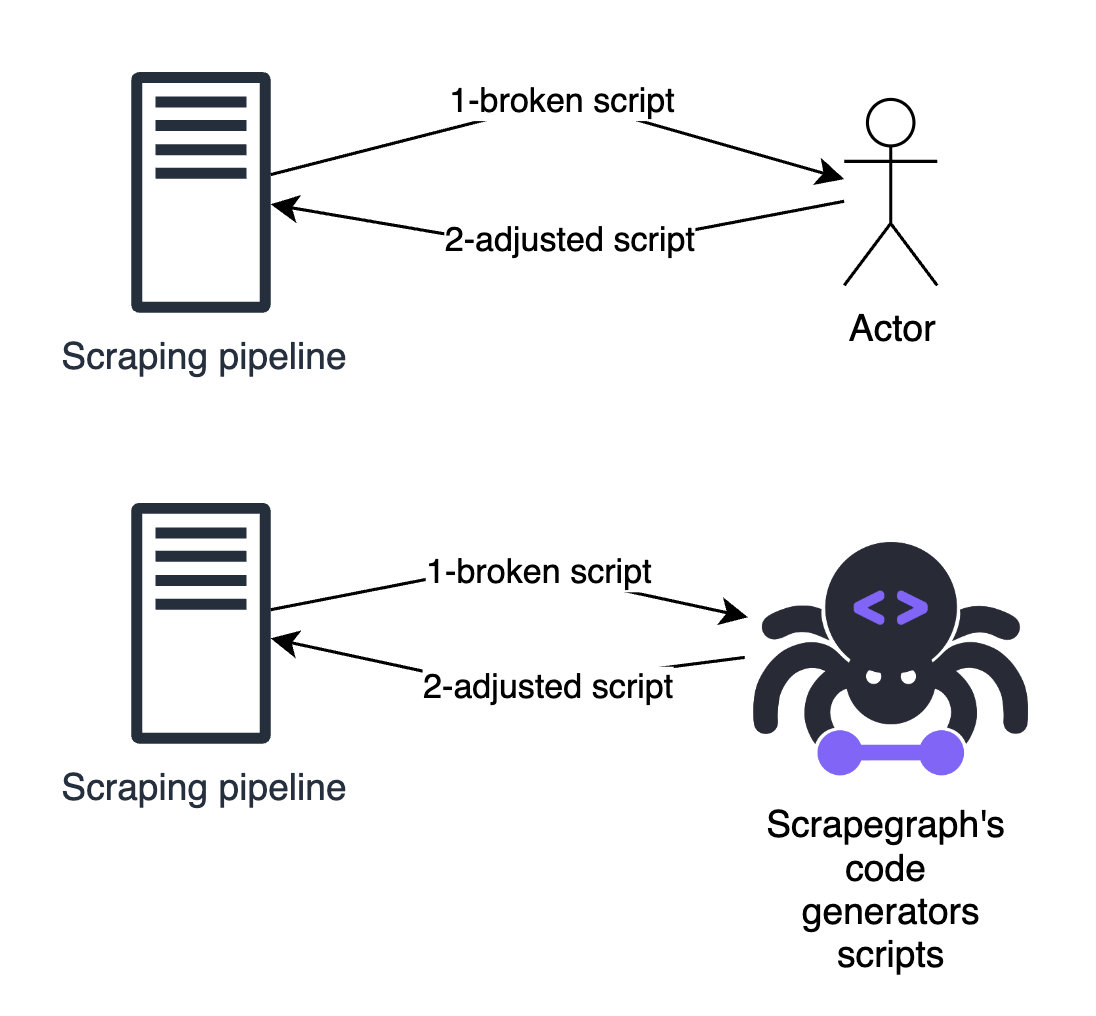
\includegraphics[width=1\linewidth]{Assets/code_generator_scripts.png}
    \caption{Functioning of code generator scripts}
    \label{fig:actually indians}
\end{figure}
\subsubsection{Script\_generator\_graph}
It a graph whose output is a python code in Beautifoulsoup given a link, a prompt and an optional schema as a input.

The elements of the graph are:

\begin{itemize}
    \item \textbf{fetch\_node}: for fetching the code
    \item \textbf{parse\_node}: for removing dead code
    \item \textbf{generate\_scraper\_node}: for generating the python code
\end{itemize}

\begin{figure}
    \centering
    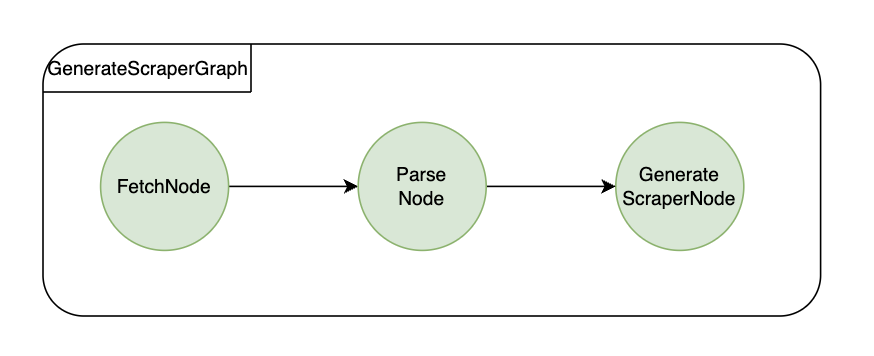
\includegraphics[width=0.85\linewidth]{Assets/generate_script_graph.png}
    \caption{generate\_scraper\_node}
    \label{fig:enter-label}
\end{figure}
\subsubsection{Code\_generator\_graph}

The Code\_generator\_graph pipeline output is the same one of the previous subsection but with a different approach. The behaviour of this graph is described in the image \ref{fig:code-generator}.

The elements of the graph are:
\begin{itemize}
    \item \textbf{fetch\_node}: for fetching the source code
    \item \textbf{parse\_node}: for improving the quality of the source code 
    \item \textbf{generate\_answer\_node}: for generating the result compliant to json format
    \item \textbf{prompt\_refiner\_node}: for making a more precise prompt
    \item \textbf{html\_analyzer\_node}: for understanding the relevants chunks of HTML code 
    \item \textbf{generate\_code\_node}: for gerating the python code for scraping
\end{itemize}

\begin{figure}[H]
    \centering
    \rotatebox{270}{
        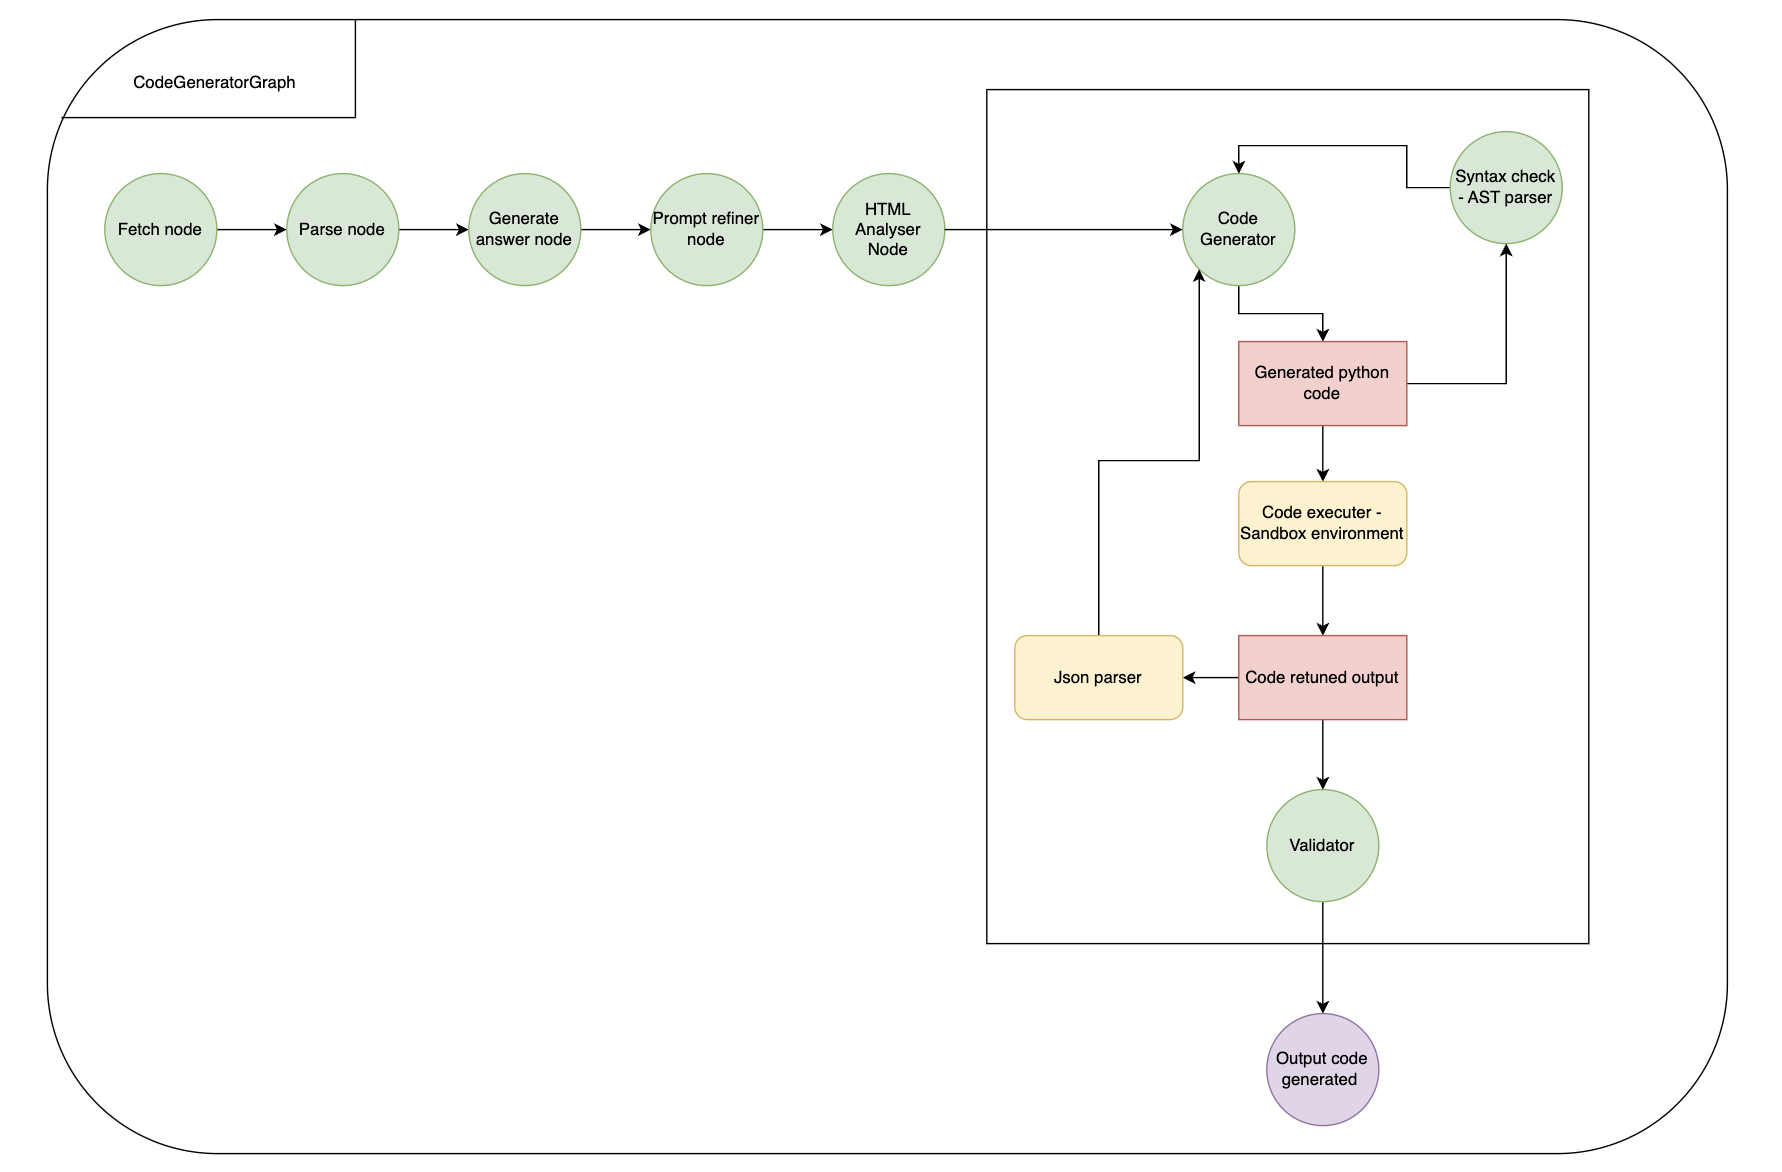
\includegraphics[width=1.25\linewidth]{Assets/code_generator.png}
    }
    \caption{Code\_generator\_graph}
    \label{fig:code-generator}
\end{figure}



\subsection{Updates management}
The successful maintenance of ScrapegraphAI , a rapidly growing open-source library, requires continuous monitoring, precise debugging, and actionable insights to sustain its performance and adaptability. In this regard, PostHog has become an indispensable tool in streamlining the library's maintenance process. As a robust product analytics platform, PostHog provides invaluable real-time insights into user interactions, feature usage, and performance bottlenecks, enabling the identification of critical areas for improvement. Crucially, PostHog’s ability to track user behavior and system events makes it particularly effective in pinpointing the exact locations of bugs within the codebase, allowing for swift and targeted resolution.

PostHog’s seamless integration with development pipelines enables comprehensive tracking of key metrics, such as error rates, user flows, and performance trends, across various releases. By automating the collection and analysis of these metrics, PostHog minimizes the manual effort involved in diagnosing and resolving issues, ensuring that problems are addressed before they escalate. For ScrapegraphAI , which operates in a fast-paced and ever-evolving environment, PostHog’s detailed analytics allow developers to maintain the library’s reliability and scalability while adhering to the high standards expected by its community.

As the owner of ScrapegraphAI , I rely on PostHog to identify and resolve bugs efficiently, ensuring the library's ongoing stability and success.

\begin{figure}[H]
    \centering
    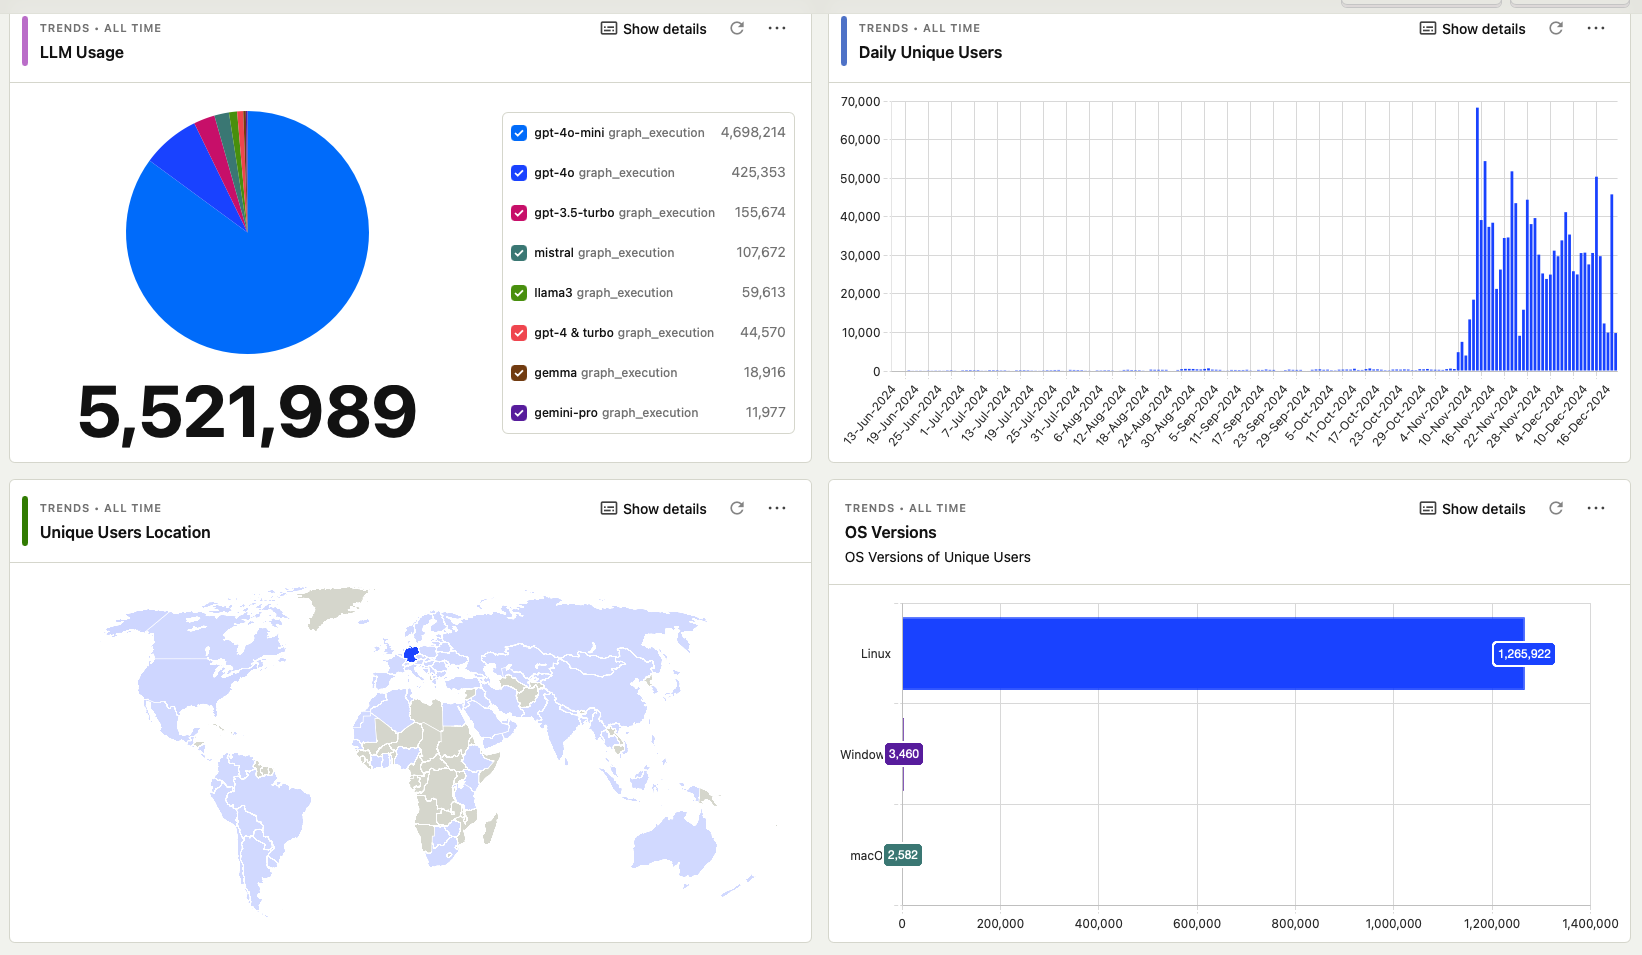
\includegraphics[width=0.95\linewidth]{Assets/posthog_dashboard.png}
    \caption{Example of Posthog dashboard}
    \label{fig:enter-label}
\end{figure}

\textbf{Fun fact}: the first day that Posthog was connected to the open source library ($17^{th}$ june 2024) it had just 1279 library's usages. The highest usage instead was done on the $21^{th}$ december 2024 with 240522 library usage

\subsubsection{Most Visited Websites}

Table~\ref{tab:most-visited-websites} presents the top 15 most frequently visited sources as of January 24, 2025. These websites represent a diverse set of industries, ranging from professional networking platforms and e-commerce to news portals and social media. The frequency values indicate the number of times data was extracted from each source using ScrapeGraphAI. This analysis highlights the versatility and widespread applicability of web scraping across various domains.

\begin{table}[H]
\centering
\begin{tabular}{|l|c|}
\hline
\textbf{Source}              & \textbf{Frequency} \\ \hline
linkedin.com                 & 18,914             \\ \hline
profesia.sk                  & 16,753             \\ \hline
adidas.se                    & 14,771             \\ \hline
localhost:8000               & 14,384             \\ \hline
m.stock.naver.com            & 13,508             \\ \hline
nytimes.com                  & 12,532             \\ \hline
google.com                   & 10,211             \\ \hline
baike.baidu.com              & 9,970              \\ \hline
derstandard.at               & 9,865              \\ \hline
ndtvprofit.com               & 9,809              \\ \hline
faz.net                      & 9,587              \\ \hline
livemint.com                 & 9,110              \\ \hline
naturitas.es                 & 8,587              \\ \hline
web.archive.org              & 8,022              \\ \hline
r.jina.ai                    & 7,764              \\ \hline
\end{tabular}
\caption{Top 15 most frequently visited websites as of January 24, 2025}
\label{tab:most-visited-websites}
\end{table}

\paragraph{Commentary}
The data in Table~\ref{tab:most-visited-websites} reveals several interesting trends:
\begin{itemize}
    \item \textbf{Professional and Informational Platforms}: \texttt{linkedin.com} and \texttt{nytimes.com} rank highly, demonstrating the importance of professional networking and trusted news sources in data scraping.
    \item \textbf{E-Commerce and Retail}: Platforms like \texttt{adidas.se} and \texttt{m.stock.naver.com} emphasize the focus on extracting product information, pricing, and stock updates.
    \item \textbf{Search Engines and Reference Sites}: \texttt{google.com} and \texttt{baike.baidu.com} highlight the use of search engines and encyclopedic resources for data retrieval and enrichment.
    \item \textbf{Dynamic and Region-Specific Sources}: \texttt{profesia.sk} and \texttt{derstandard.at} reflect the geographic diversity of web scraping applications, catering to localized needs.
\end{itemize}

The high frequency of these sources underscores the widespread reliance on ScrapeGraphAI for data extraction across varied industries and content types. This analysis also illustrates the dynamic nature of web scraping, with sources ranging from static content repositories to dynamically updated platforms.

\begin{figure}[H]
    \centering
    \includegraphics[width=\textwidth]{Screenshot_2025-01-24_alle_15.21.13.png}
    \caption{Geographic distribution of web scraping activity frequencies as of January 24, 2025. The color scale represents the intensity of scraping activity, with darker purple indicating lower activity and bright yellow representing the highest frequency.}
    \label{fig:geographic-distribution}
\end{figure}

\paragraph{Image Commentary}
Figure~\ref{fig:geographic-distribution} provides a visual representation of web scraping activity across various regions. Key observations include:
\begin{itemize}
    \item \textbf{High Activity Regions}: North America and South Asia display the most intense scraping activity, as evidenced by the bright yellow regions.
    \item \textbf{Moderate Activity}: Europe shows moderate levels of scraping, reflecting its diverse digital ecosystem.
    \item \textbf{Low Activity}: Regions like Africa and parts of South America have significantly lower scraping frequencies, potentially due to limited internet infrastructure or lower digital presence.
\end{itemize}

This global distribution highlights the geographical diversity and varying levels of activity in web scraping operations.

\begin{figure}[H]
    \centering
    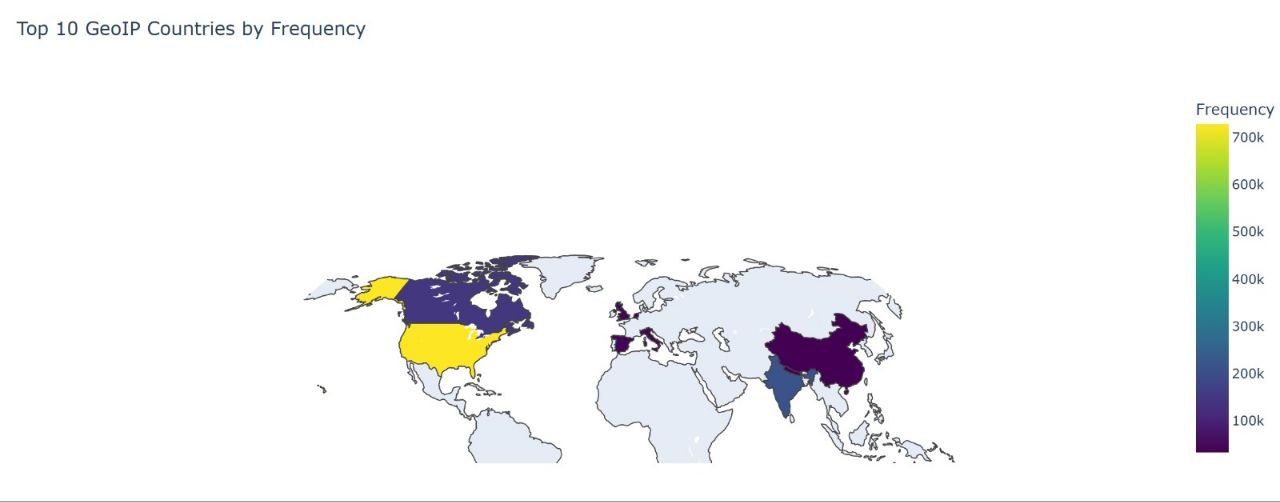
\includegraphics[scale=0.25]{Assets/countries.jpg}
    \caption{geographic distribution}
    \label{fig:geographic-distribution}
\end{figure}

\begin{figure}[H]
    \centering
    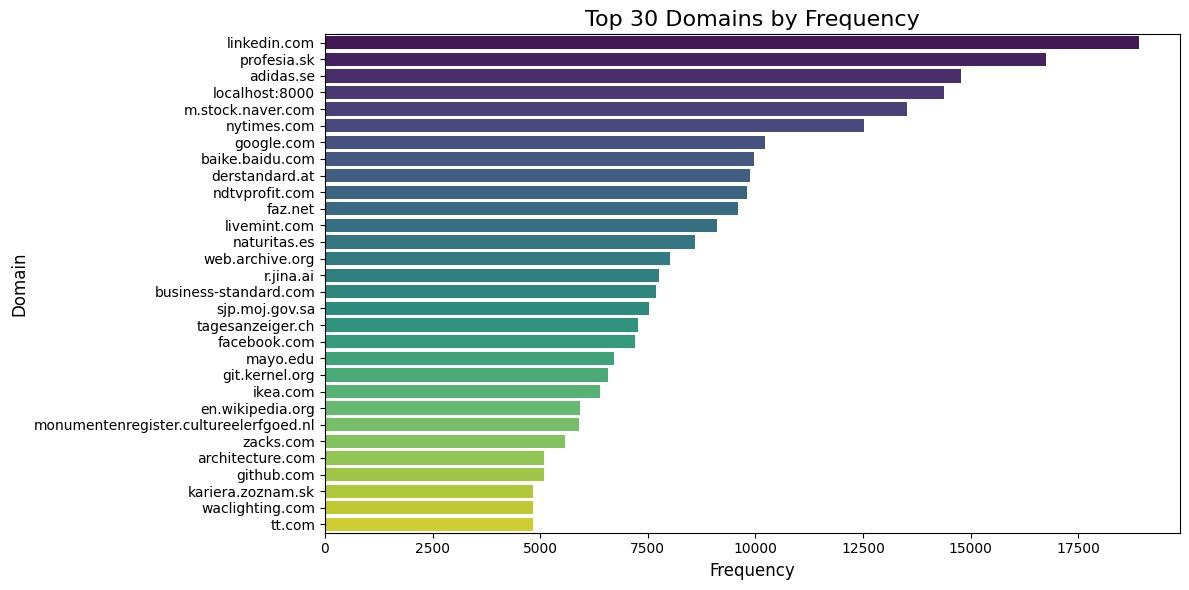
\includegraphics[scale=0.45]{Assets/websites.jpg}
    \caption{Caption}
    \label{fig:enter-label}
\end{figure}
\section{What makes ScrapegraphAI  cool}
\subsection{Available LLM Models}

ScrapegraphAI is fully compatible with all the principal LLM models available on the market. The most well-known providers include OpenAI, Mistral, Gemini, Meta (LLaMA), and Groq. Ensuring compatibility with multiple models is crucial for maximizing flexibility, performance, and adaptability in various scraping and data extraction scenarios.

\subsubsection{Why Supporting Multiple LLM Versions is Important}

The rapid evolution of large language models (LLMs) has led to continuous improvements in accuracy, efficiency, and contextual understanding. Supporting all available versions of LLMs in ScrapegraphAI provides several strategic advantages:

\begin{itemize}
    \item \textbf{Performance Optimization}: Different models excel in various tasks—some are optimized for speed (e.g., Groq), while others focus on accuracy and depth of reasoning (e.g., GPT-4o). ScrapegraphAI users can select the best model for their specific needs.
    \item \textbf{Cost Efficiency}: Newer LLM versions often come with pricing adjustments. By supporting multiple versions, ScrapegraphAI allows users to balance performance and cost-effectiveness by choosing older or lightweight models when high computational power is unnecessary.
    \item \textbf{Resilience and Redundancy}: Relying on a single provider increases the risk of disruptions due to API changes, model deprecations, or service downtimes. Multi-model support ensures that ScrapegraphAI remains functional even if one provider experiences technical issues.
    \item \textbf{Task-Specific Adaptation}: Some scraping tasks require specific LLM capabilities. For example, Meta’s LLaMA models might be more efficient for multilingual content, while OpenAI’s GPT-4o may be better suited for reasoning-intensive tasks.
    \item \textbf{Compliance and Data Privacy}: Different organizations have varying data governance policies. By offering multiple LLM choices, ScrapegraphAI enables users to select models that align with their privacy, security, and regulatory requirements.
\end{itemize}

\subsubsection{Future-Proofing ScrapeGraph}

LLM technology is evolving at an unprecedented pace, with new models frequently released and older ones being deprecated. Maintaining support for all available versions ensures that ScrapegraphAI remains compatible with cutting-edge advancements while providing users with the flexibility to transition seamlessly between models without disrupting their workflows.

By integrating multiple LLM providers and versions, ScrapegraphAI empowers users with unparalleled flexibility, reliability, and efficiency, making it a robust solution for AI-driven web scraping and data extraction.
\section{Step-by-step guide}
In this section it will be showed a tutorial for scraping with both library and APIs showing an use case of a data extraction of an e-commerce.

For simplicity, the following link: \textit{\url{https://www.amazon.it/s?k=keyboard&__mk_it_IT=ÅMÅŽÕÑ&crid=2NTE6199MWOQE&sprefix=keyboar\%2Caps\%2C114&ref=nb_sb_noss_2V}}

will be written as \textit{\url{https://www.amazon.it/s?k=keyboard}}.

\subsection{Open source library}

To begin using the open-source library, you should visit the following GitHub repository: \url{https://github.com/ScrapeGraphAI/ScrapegraphLib-Examples/blob/main/openai/smart_scraper_openai.py}. In this example, you may need to specify an output schema using Pydantic to ensure the data is structured properly. This allows for smooth integration with the scraping pipeline.

Here is an example of how you can use the SmartScraper library in Python:

\begin{figure}[H]
    \centering
    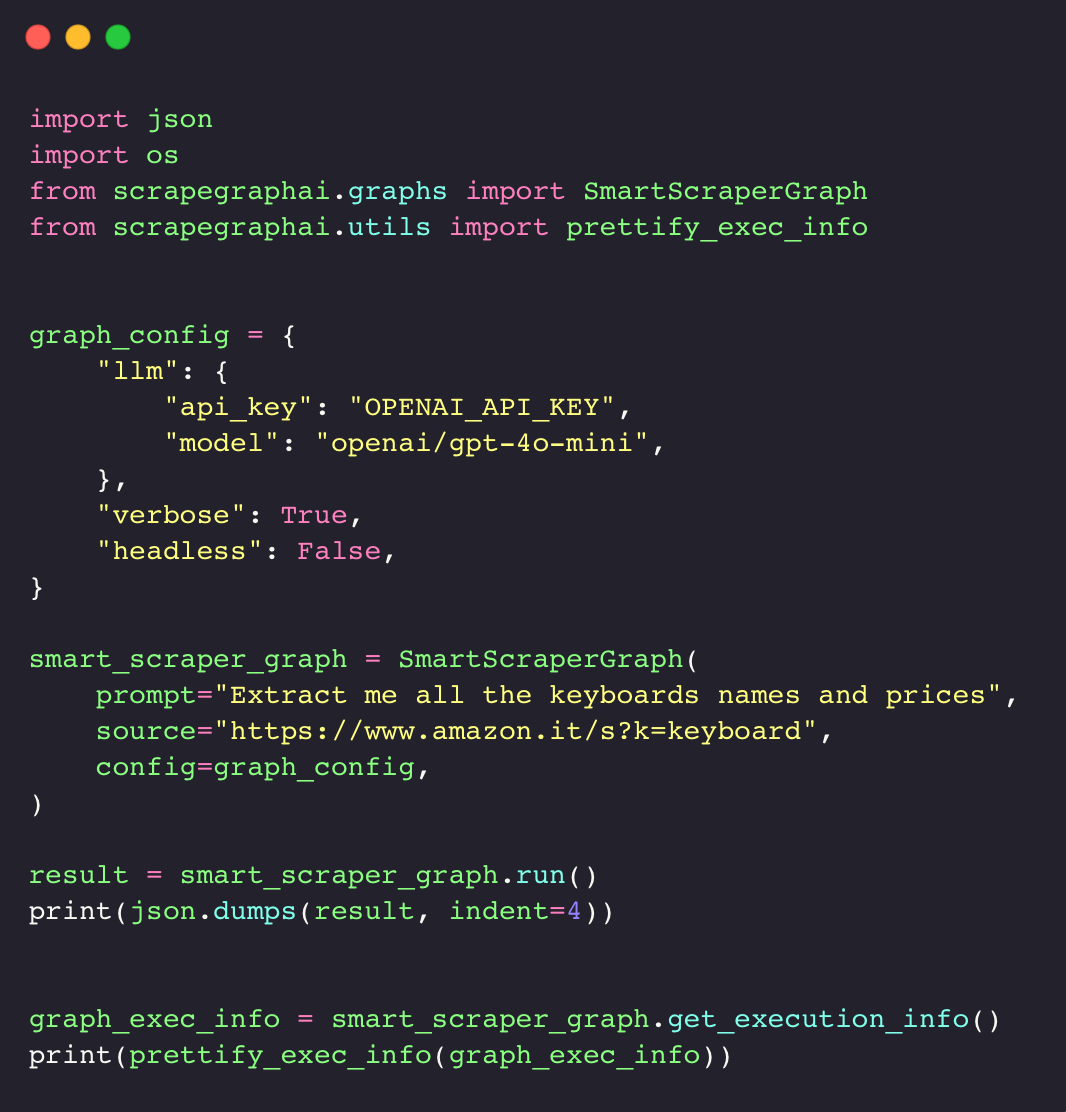
\includegraphics[width=0.95\linewidth]{Assets/library.png}
    \caption{Code required for scraping Amazon with official library}
    \label{fig:enter-label}
\end{figure}

This code snippet demonstrates how to define the configuration for the SmartScraperGraph, run the scraper on Amazon's website, and retrieve the execution results. You can modify the `prompt` and `source` parameters to scrape different websites or data.

\subsection{Official APIs}

For those who prefer to use the official APIs, it is possible to find detailed documentation on how to set up the SmartScraper at \url{https://docs.scrapegraphai.com/services/smartscraper}. 
To use the SmartScraper API, start by getting the API key from \url{https://dashboard.scrapegraphai.com}.

After that, the Client should be imported as follows:

\begin{figure}[H]
    \centering
    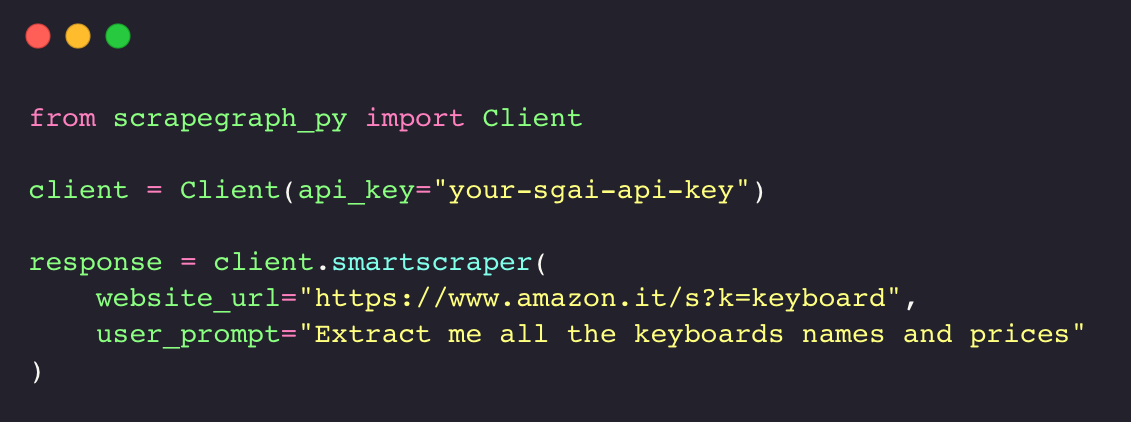
\includegraphics[width=0.95\linewidth]{Assets/api.png}
    \caption{Code required for scraping Amazon with APIs}
    \label{fig:enter-label}
\end{figure}

In this case, the website to scrape is Amazon. The SmartScraper allows you to define the URL to scrape, along with a prompt for the type of information you want to extract. You can customize this further based on your needs.

\section{Benchmarks}

ScrapeGraph's traction over the past few months has been incredible, thanks to the supportive community behind it.

What started as a tool to simplify complex data scraping quickly evolved into a collaborative platform. Users shared their experiences, provided feedback, and contributed ideas, fostering continuous improvement. Professionals from diverse industries connected, offering unique insights and challenges that inspired new features. This collaboration has transformed ScrapeGraphAI into more than just a tool—it is now a community-driven project shaped by its users, each contributing to its growth and impact.

\subsection{LLM-Based Extraction Benchmarking}

When testing LLM-based extraction methods, OpenAI's GPT-4o was the provider of choice. The website wired.com served as an ideal benchmark due to its complex structure, balancing data volume with the challenge of extracting both tags and metadata effectively. This ensured comprehensive tests covering real-world challenges in web scraping and data parsing.

For larger-scale tests or scaling content extraction, the following steps were implemented:

\begin{enumerate}
    \item \textbf{Enhancing Metadata Extraction:}
    \begin{itemize}
        \item Implement advanced parsing techniques for improved handling of structured and unstructured data.
        \item Address deeply nested tags and dynamically loaded content for comprehensive metadata capture.
    \end{itemize}
    
    \item \textbf{Balancing Extraction Load:}
    \begin{itemize}
        \item Introduce parallel data requests and batch processing to optimize workload management.
        \item Utilize retry mechanisms with exponential backoff to ensure uninterrupted extraction.
    \end{itemize}
    
    \item \textbf{Benchmark Evaluation:}
    \begin{itemize}
        \item Set up automated tests comparing extracted data accuracy and completeness with ground truth data.
        \item Evaluate performance on wired.com, walmart.com, ikea.com, and nature.com, focusing on processing speed and metadata completeness.
    \end{itemize}
\end{enumerate}

This approach ensured better scalability and robustness in data extraction with LLMs.

\begin{figure}[H]
    \centering
    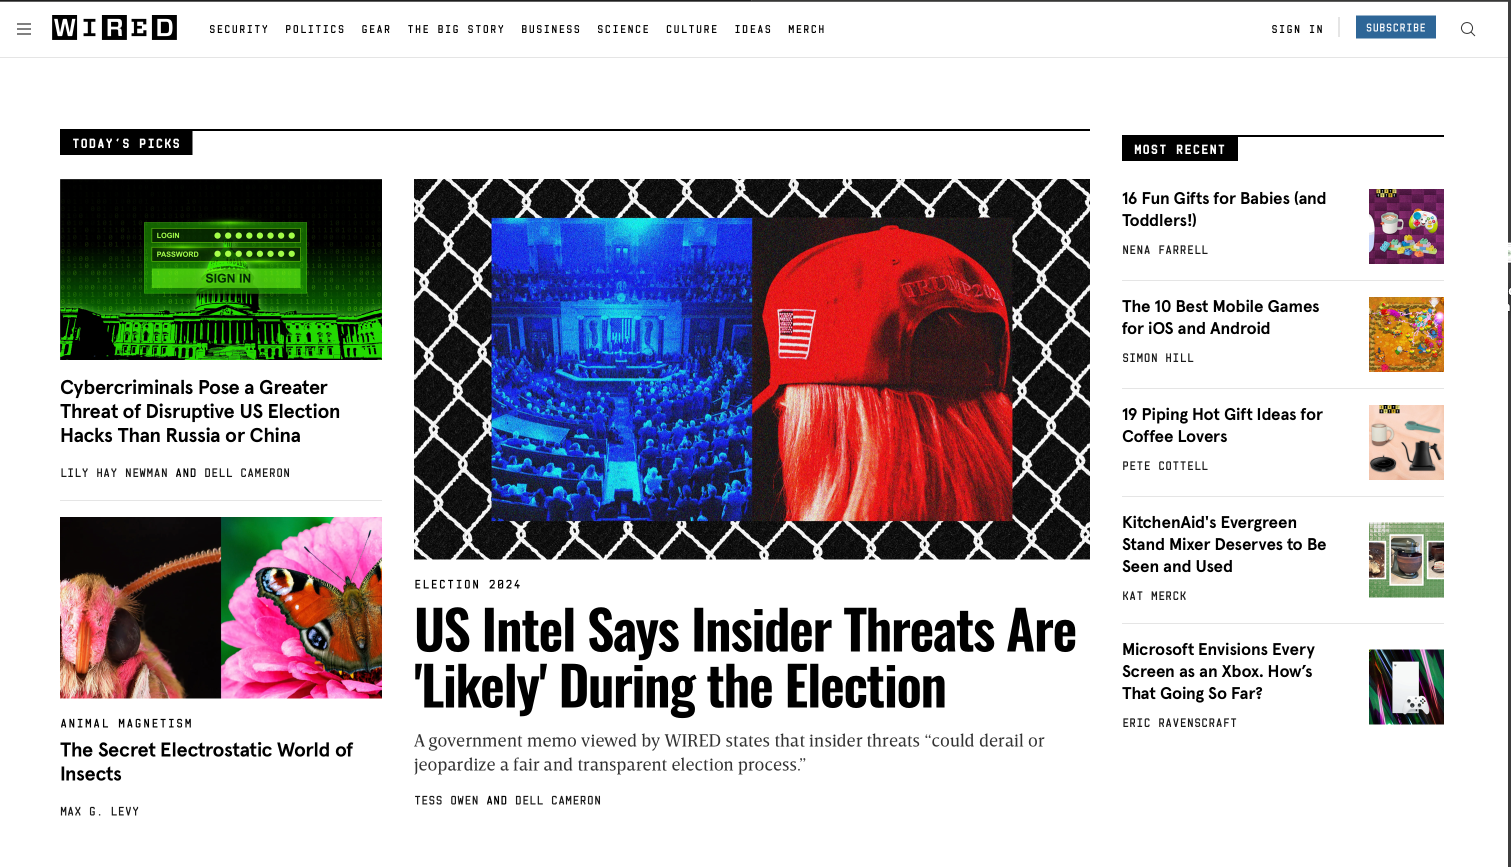
\includegraphics[width=0.95\linewidth]{Assets/wired.png}
    \caption{Wired.com website as of 28/10/2024}
    \label{fig:enter-label}
\end{figure}

The expected result format is shown in Figure~\ref{fig:res-snippet}, where \texttt{title}, \texttt{author}, and \texttt{url} are keys.

For all ScrapeGraphAI tests, the following prompts were used:

\begin{itemize}
    \item \textbf{wired.com}: ``\textit{Extract all the articles}''
    \item \textbf{walmart.com}: ``\textit{Extract the product names}''
    \item \textbf{ikea.com}: ``\textit{Extract the product names}''
    \item \textbf{nature.com}: ``\textit{Extract the articles}''
\end{itemize}

\begin{figure}[H]
    \centering
    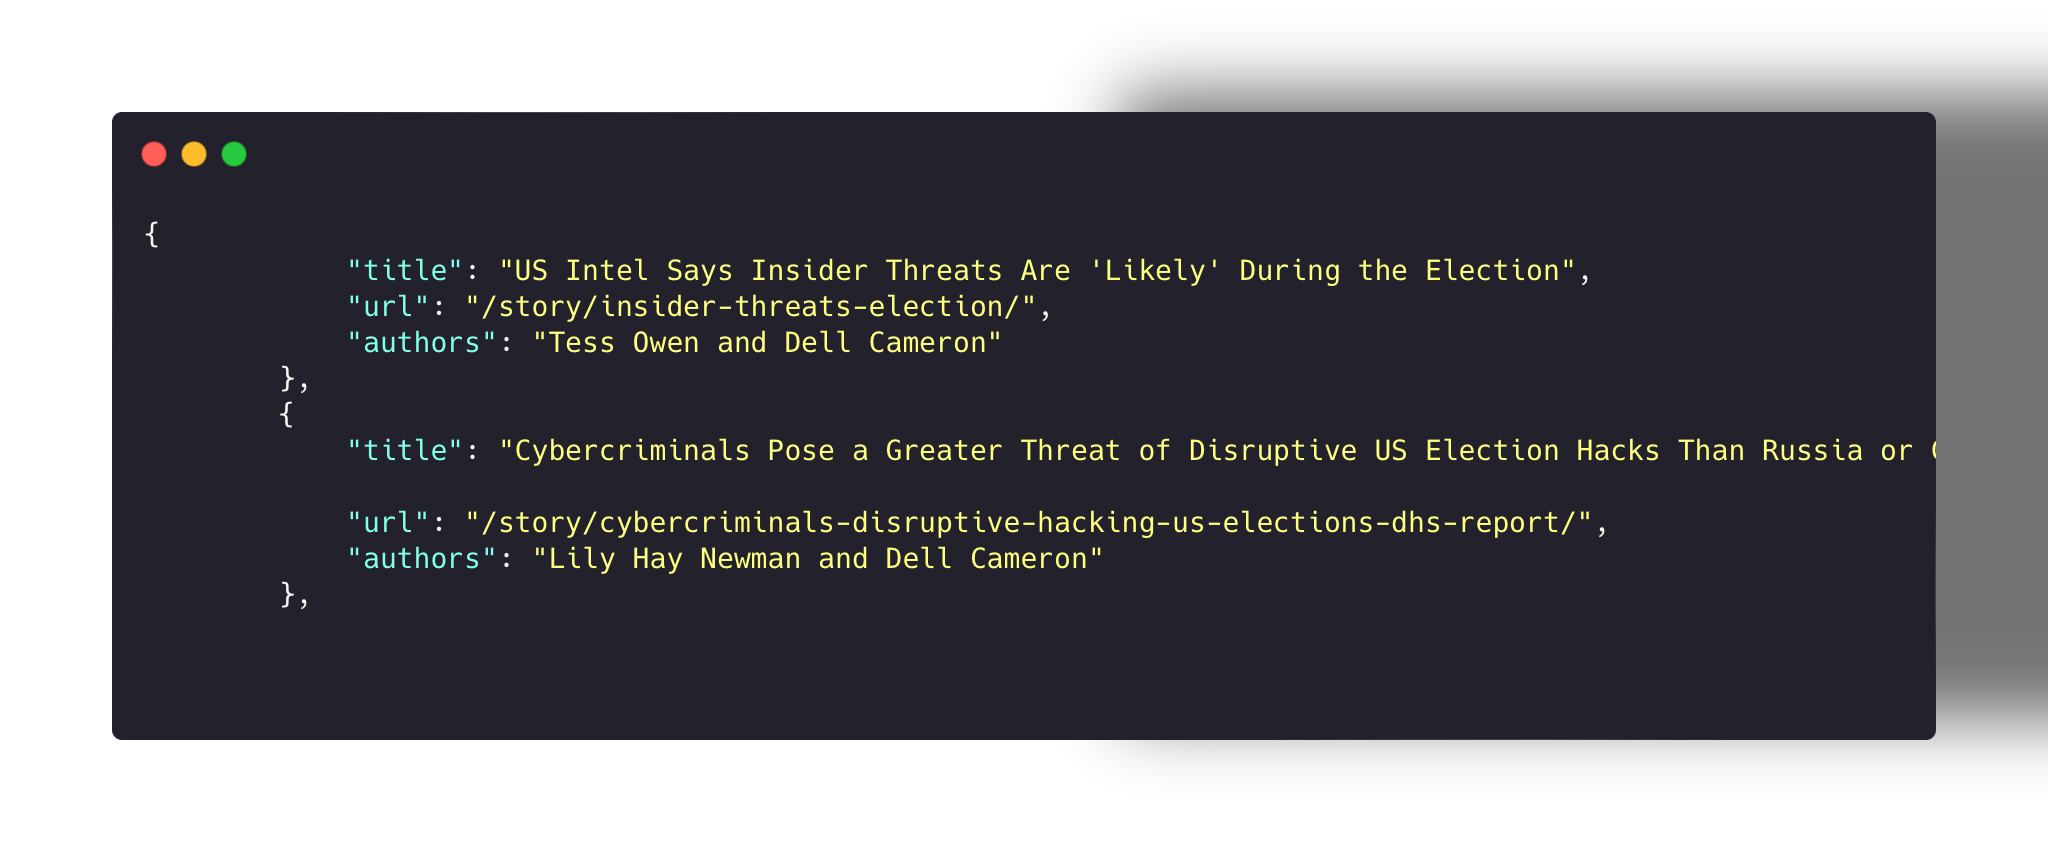
\includegraphics[width=0.95\linewidth]{Assets/result.png}
    \caption{Result snippet format}
    \label{fig:res-snippet}
\end{figure}

\section{Setup Time}

\subsection{ScrapeGraphAI}
Setting up ScrapeGraphAI was quick and straightforward, taking only a few minutes. The process involved copying and pasting the example folder into the project directory and adjusting the prompt to match the desired extraction task. If initial results were unsatisfactory, modifications could be made easily by tweaking the prompt or output format without rewriting the extraction logic. ScrapeGraphAI automates the complexity of parsing various website structures, making it highly efficient for large-scale data extraction tasks.

\subsection{BeautifulSoup}
Setting up BeautifulSoup required significantly more time and effort. The process began with manually inspecting each website's HTML structure to identify relevant elements such as article titles, product names, authors, or metadata. This involved analyzing the Document Object Model (DOM), finding correct CSS selectors or XPath expressions, and ensuring compatibility across pages.

Next, a custom web scraper was implemented to fetch and parse HTML content. Handling edge cases, such as dynamically loaded content, inconsistent tag structures, and anti-scraping mechanisms, added to the complexity. Debugging and refining the script for improved accuracy further extended the setup time.

Overall, achieving comparable results with BeautifulSoup often took several hours or even a full day, depending on the website's complexity. Unlike ScrapeGraphAI, which abstracts low-level processing, BeautifulSoup demands a deep understanding of HTML parsing and requires continuous maintenance as website structures change.

\section{Balancing Extraction Load and Inference Time}

Efficiently managing extraction load is a fundamental challenge in large-scale web scraping. The performance of a web scraping framework depends on its ability to handle diverse website structures while maintaining reasonable inference times. Table~\ref{tab:comparison} provides a comparative analysis of inference times for ScrapeGraphAI and BeautifulSoup across multiple websites, offering valuable insights into their performance characteristics.

The results highlight that BeautifulSoup, due to its direct interaction with the Document Object Model (DOM) and minimal abstraction layers, achieves faster processing times. For example, websites like Wired.com and Walmart.com demonstrate a clear speed advantage when using BeautifulSoup, with inference times of 11.70 seconds and 15.87 seconds, respectively. However, this speed comes with a trade-off: BeautifulSoup often requires significant development time and technical expertise to handle complex website structures.

ScrapeGraphAI, in contrast, demonstrates slightly longer inference times—such as 15.20 seconds for Wired.com and 20.89 seconds for Walmart.com. This additional time is attributed to its abstraction layers and advanced automation capabilities, which simplify setup and enable broader adaptability to dynamic or deeply nested content, as seen on websites like Ikea.com and Nature.com.

For websites with complex or dynamic content, such as Ikea.com and Nature.com, both tools exhibit increased processing times due to the need for handling JavaScript-rendered elements and deeply nested structures. These cases underscore the importance of implementing strategies like parallelizing requests and batch processing to optimize extraction performance. Additionally, integrating robust retry mechanisms, such as exponential backoff, ensures continuity in data extraction tasks, mitigating the impact of network fluctuations or temporary server blocks.

Ultimately, the choice between BeautifulSoup and ScrapeGraphAI depends on the specific requirements of the task. While BeautifulSoup excels in speed for simpler tasks, ScrapeGraphAI's flexibility and automation make it the superior choice for projects requiring scalability, adaptability, and rapid development.
\section{Benchmark Evaluation}

\subsection{Accuracy}

For both methods, the results were accurate. Each method was tested over 100 runs, and the reported times represent the average. The repository used for these tests is available at: \url{https://github.com/VinciGit00/master-thesis-scraping}.

To evaluate the accuracy of both methods, tests were conducted over 100 runs for each website. The extracted data was compared against manually verified ground truth data to ensure completeness and correctness. Both ScrapeGraphAI and BeautifulSoup produced highly accurate results, with no significant discrepancies observed.

BeautifulSoup's accuracy depends heavily on the quality of manually crafted selectors or XPath expressions, making it prone to errors if website structures are updated. Conversely, ScrapeGraphAI leverages large language models (LLMs) to adapt to such changes dynamically, maintaining accuracy even in the face of structural variations.


\section{Scripts}

The repository is organized into two main scripts, each serving a specific purpose in the web scraping process:

\subsection{smart\_scraper.py}

This script is responsible for the core web scraping operations. It utilizes the ScrapeGraphAI library, which leverages Large Language Models (LLMs) and direct graph logic to create scraping pipelines for websites and local documents (XML, HTML, JSON, Markdown, etc.). The script is structured as follows:

\begin{itemize}
    \item \textbf{Initialization:} Imports necessary modules and sets up configurations for the scraping process.
    \item \textbf{Proxy Management:} Implements proxy rotation to ensure anonymity and prevent IP blocking during scraping.
    \item \textbf{Data Extraction:} Defines functions to extract specific data points from the target websites using ScrapeGraphAI's capabilities.
    \item \textbf{Data Storage:} Processes and stores the extracted data in a structured format, such as CSV or JSON, for further analysis.
\end{itemize}

This organization allows for efficient and scalable web scraping operations, leveraging the advanced features of the ScrapeGraphAI library.

\subsection{beautifousoup.py}

This script focuses on parsing and navigating HTML documents using the BeautifulSoup library. It is structured as follows:

\begin{itemize}
    \item \textbf{Initialization:} Imports the BeautifulSoup module and other necessary libraries.
    \item \textbf{HTML Parsing:} Defines functions to parse HTML content and extract specific elements based on tags, classes, or IDs.
    \item \textbf{Data Processing:} Processes the extracted data to clean and structure it appropriately.
    \item \textbf{Data Storage:} Saves the processed data in a desired format for further use.
\end{itemize}

The integration of BeautifulSoup allows for precise extraction of data from HTML documents, complementing the functionalities provided by ScrapeGraphAI.

\begin{figure}[H]
    \centering
    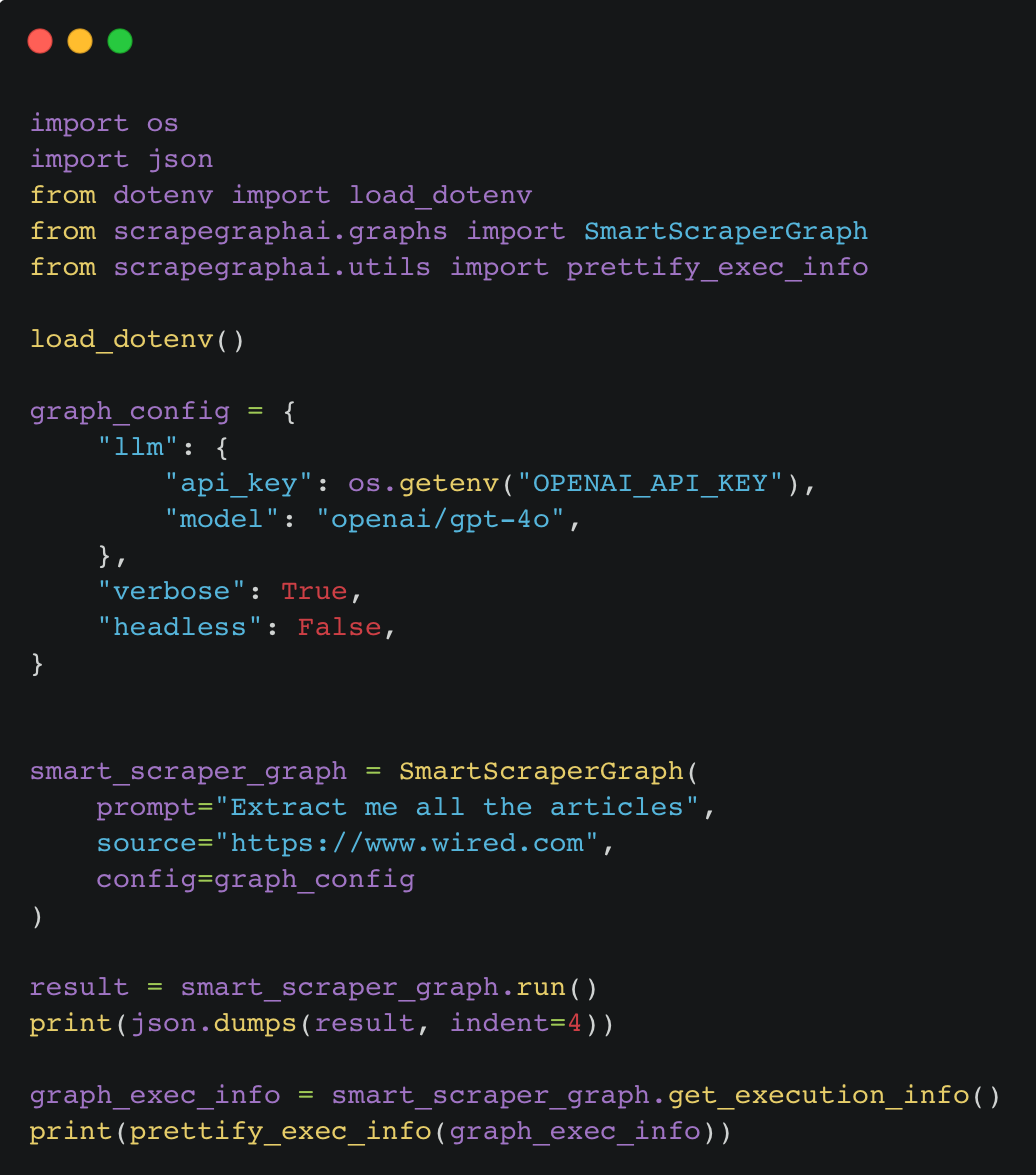
\includegraphics[width=0.95\linewidth]{Assets/smart_scraper_wired.png}
    \caption{Snippet of ScrapeGraphAI snippet integration}
    \label{fig:smart_scraper_wired}
\end{figure}

\begin{figure}[H]
    \centering
    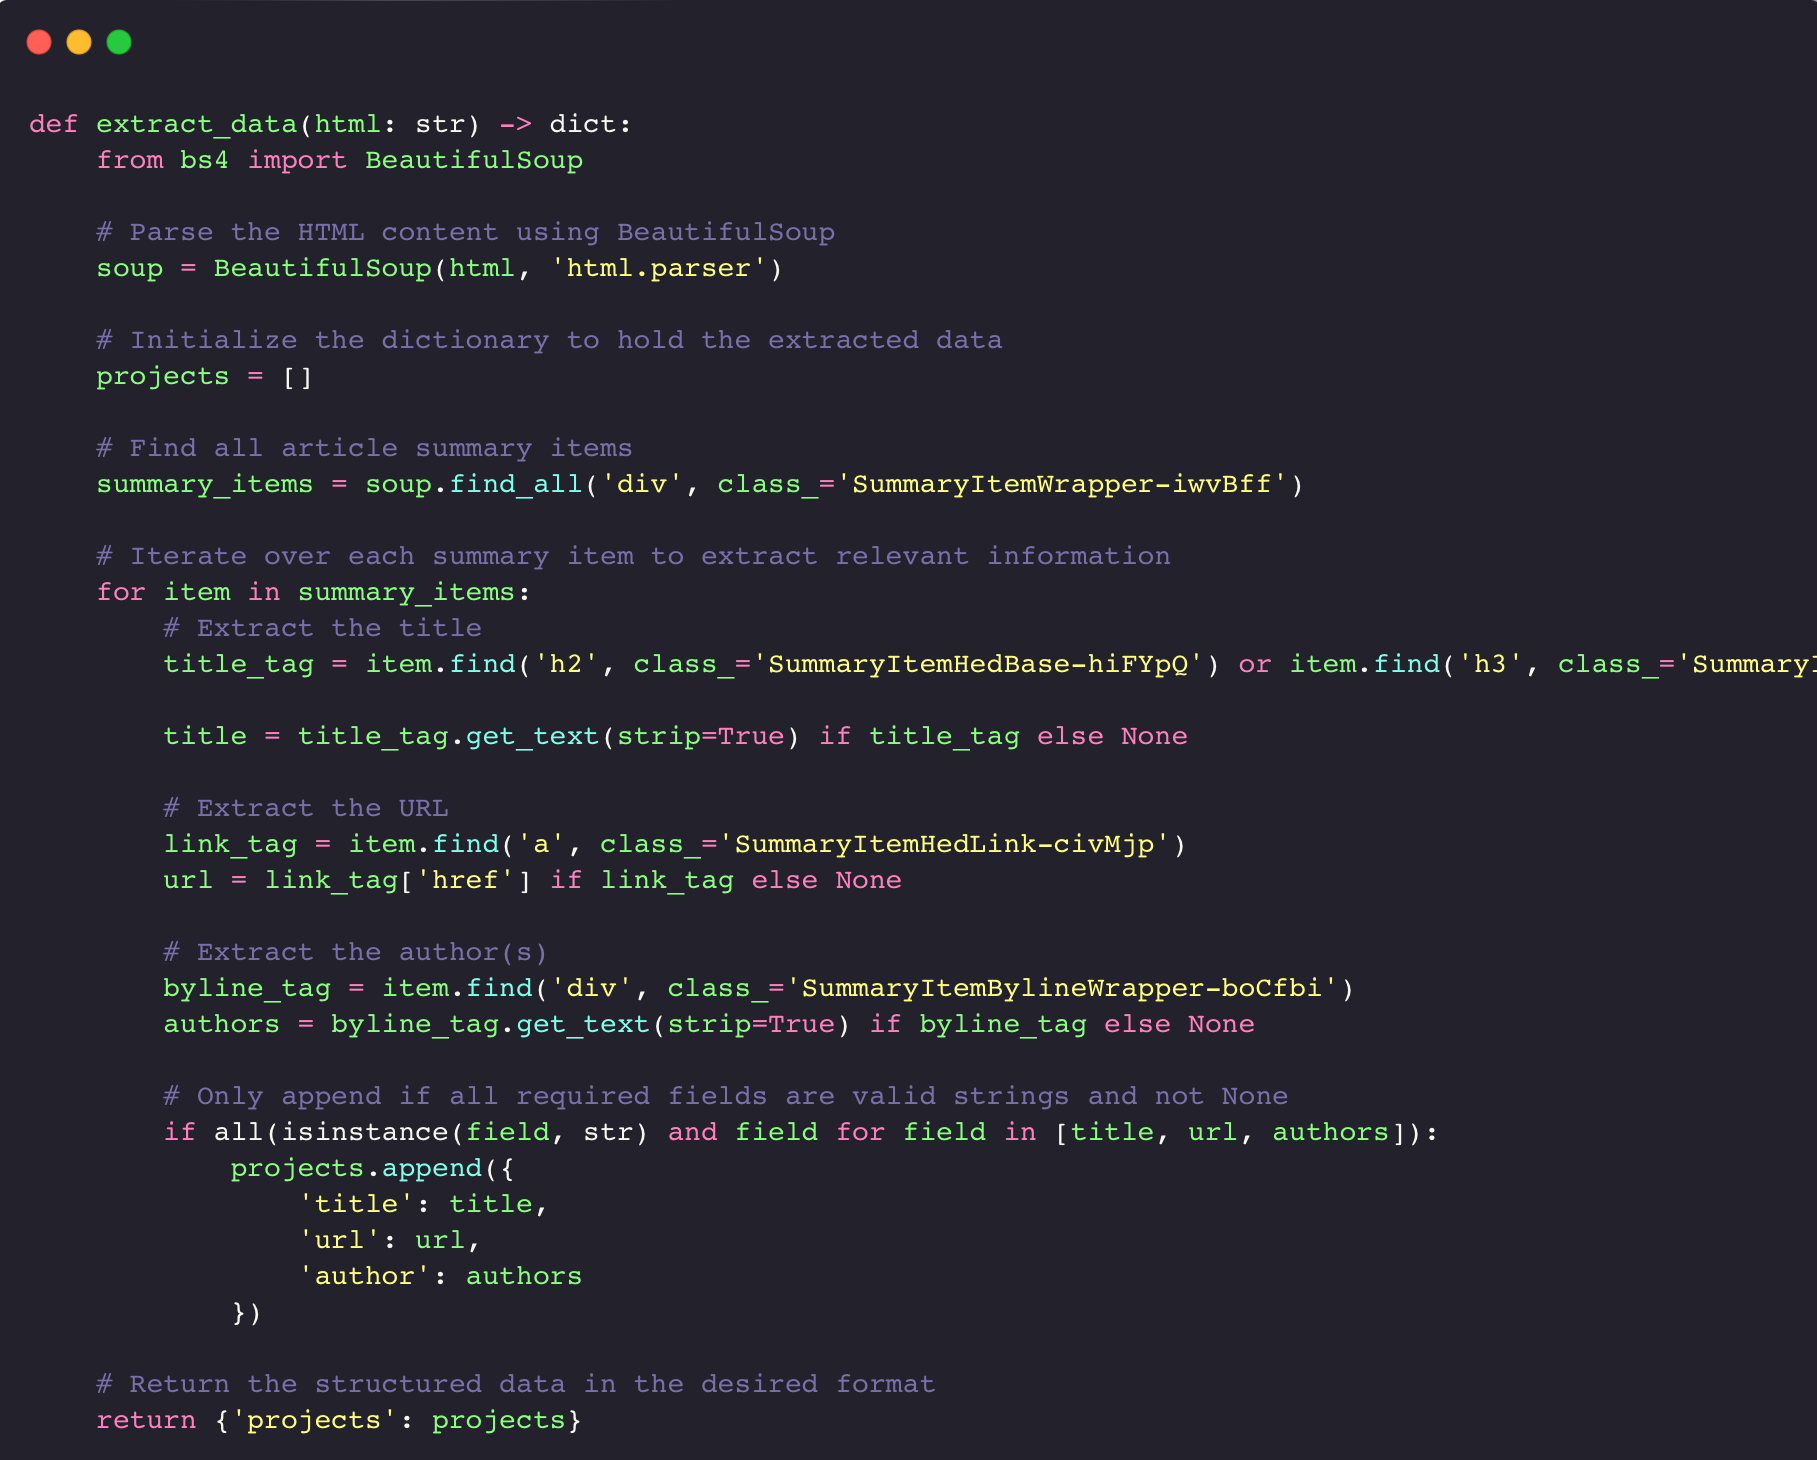
\includegraphics[width=0.95\linewidth]{Assets/beautifousoup.png}
    \caption{Snippet of BeautifulSoup snippet integration}
    \label{fig:beautifousoup}
\end{figure}

\subsection{Integration and Workflow}

The scripts are designed to be modular, allowing for flexibility in the scraping process. The \texttt{smart\_scraper.py} script can operate independently, utilizing the ScrapeGraphAI library for advanced scraping tasks. Alternatively, it can integrate with the \texttt{beautifousoup.py} script to handle specific HTML parsing requirements, providing a comprehensive solution for web scraping needs.

This modular approach ensures that the system can adapt to various scraping scenarios, leveraging the strengths of both the ScrapeGraphAI and BeautifulSoup libraries.

\section{Comparison with ScrapegraphAI APIs}
From November 2024, the official API was released. They provide greater efficiency in terms of time, accuracy, and integration, especially with proxy rotation for fetching. This was the first release of the paid service, and as shown in Table \ref{tab:comparison}, the inference time is lower compared to the library.

\begin{table}[h!]
\centering
\begin{tabular}{|l|c|c|c|c|}
\hline
                & Wired.com & Walmart.com & Ikea.com & nature.com \\ \hline
ScrapegraphAI APIs   &    20.0 s      &  27.99 s    &  27.56 s & 16.86 s            \\ \hline
\end{tabular}
\caption{Inference time API}
\label{tab:comparison}
\end{table}

\newpage

\subsection{Advantages of Using ScrapegraphAI APIs Over the Python Library}

1. \textbf{Increased Efficiency in Time}  
   The APIs provide faster inference times compared to the Python library. As shown in Table \ref{tab:comparison}, the response times from the API are significantly quicker, leading to overall time savings in data fetching.

2. \textbf{Improved Accuracy}  
   The APIs are optimized for better accuracy, reducing the risk of errors during data retrieval compared to the Python library.

3. \textbf{Better Integration and Proxy Rotation}  
   The official APIs come with built-in proxy rotation mechanisms, making it easier to manage large-scale data extraction without the need to manually handle proxy configurations, which is more cumbersome in the Python library.

4. \textbf{Scalability}  
   With the APIs, it's easier to scale up operations without worrying about local resource limitations. They can handle higher traffic loads efficiently, allowing users to focus more on the results rather than infrastructure management.

5. \textbf{Reduced Maintenance}  
   The API removes the burden of maintaining complex scraping logic, which is part of the Python library, ensuring that updates and bug fixes are handled on the server side.

6. \textbf{Better Resource Allocation}  
   By offloading the scraping process to the API, users free up local resources for other tasks, such as data analysis and processing, instead of managing the scraping infrastructure.

7. \textbf{Simplified Workflow}  
   APIs provide a more straightforward and standardized way to fetch data, reducing the complexity of integrating with different websites and handling edge cases directly within the scraping logic.

\section{Real-World Applications}

Web scraping, powered by advanced frameworks like ScrapeGraphAI, is an essential tool across numerous industries. By automating the extraction and processing of vast amounts of data, it allows businesses, researchers, and organizations to unlock actionable insights, streamline operations, and innovate in ways that were previously impossible. This section explores in depth the real-world applications of web scraping and the transformative role of ScrapeGraphAI in addressing complex challenges.

\subsection{E-Commerce and Retail}
The e-commerce and retail sectors heavily rely on web scraping to stay competitive in a fast-paced market. ScrapeGraphAI empowers businesses to automate data collection, enabling them to:
\begin{itemize}
    \item \textbf{Dynamic Pricing Strategies}: Retailers can monitor competitors’ pricing in real time, adjusting their own prices to remain competitive and maximize profit margins. For instance, an online electronics store can compare prices of similar products across multiple platforms and adjust pricing dynamically based on market conditions.
    \item \textbf{Demand Forecasting}: By analyzing customer behavior, reviews, and historical sales data, businesses can anticipate trends, manage inventory effectively, and avoid stock shortages or overstocking.
    \item \textbf{Sentiment Analysis}: Scraping customer reviews and social media comments allows companies to assess consumer sentiment toward their products and services. This insight enables targeted marketing campaigns and improved customer satisfaction.
    \item \textbf{Product Availability Monitoring}: Businesses can track the availability of specific items on competitors’ websites to identify opportunities for market entry or pricing adjustments.
\end{itemize}
For example, Amazon sellers can integrate ScrapeGraphAI to analyze market trends, monitor competing listings, and refine their product strategies, saving significant time and resources.

\subsection{Market Research and Analytics}
Market research firms benefit immensely from web scraping tools to collect and analyze data from a variety of sources. ScrapeGraphAI simplifies this process by automating complex workflows, such as:
\begin{itemize}
    \item \textbf{Competitive Analysis}: Gathering data on competitors’ products, pricing, and promotional strategies to create detailed reports for clients.
    \item \textbf{Trend Analysis}: Identifying emerging industry trends by scraping news articles, social media platforms, and discussion forums.
    \item \textbf{Consumer Insights}: Extracting data from surveys, reviews, and online discussions to understand consumer preferences, purchase behavior, and unmet needs.
\end{itemize}
For example, a market research firm analyzing the rise of plant-based food products can use ScrapeGraphAI to aggregate data from blogs, online grocery stores, and social media platforms, gaining a holistic understanding of the trend.

\subsection{Healthcare and Life Sciences}
The healthcare industry generates massive amounts of data daily, much of which resides in private repositories or scientific publications. ScrapeGraphAI facilitates the extraction and processing of this data for applications such as:
\begin{itemize}
    \item \textbf{Medical Research}: Mining scientific articles, clinical trial databases, and medical journals for the latest research developments and experimental findings.
    \item \textbf{Epidemiology}: Collecting real-time data on disease outbreaks from news sources, social media, and government reports to predict and manage public health crises.
    \item \textbf{Patient Sentiment Analysis}: Analyzing patient reviews, feedback, and ratings of healthcare services to improve the quality of care.
    \item \textbf{Pharmaceutical Analytics}: Tracking drug approvals, pricing, and availability across global markets.
\end{itemize}
For example, researchers studying the spread of a new virus strain can use ScrapeGraphAI to gather information from news reports, research papers, and government health portals, ensuring access to up-to-date data.

\subsection{Finance and Investment}
The financial sector relies on timely, accurate data to drive decisions. Web scraping tools like ScrapeGraphAI enable financial institutions and investors to:
\begin{itemize}
    \item \textbf{Stock Market Analysis}: Scrape stock prices, trading volumes, and financial news to identify trends and make informed investment decisions.
    \item \textbf{Alternative Data Analysis}: Extract non-traditional data, such as online consumer sentiment, product reviews, and social media activity, to predict market movements.
    \item \textbf{Regulatory Monitoring}: Keep track of changes in financial regulations and compliance requirements to ensure operational integrity.
\end{itemize}
For example, hedge funds can use ScrapeGraphAI to monitor news sentiment about publicly traded companies, identifying potential investment opportunities or risks.

\subsection{Education and Academia}
Researchers and educators utilize web scraping for various academic and educational purposes. ScrapeGraphAI enables:
\begin{itemize}
    \item \textbf{Dataset Generation}: Collecting data for machine learning models, such as natural language processing or image recognition systems.
    \item \textbf{Scholarly Analysis}: Mining data from open-access journals, digital libraries, and research repositories to analyze trends in academic publishing.
    \item \textbf{Online Education Platforms}: Scraping user engagement data and feedback from online learning platforms to improve educational offerings.
\end{itemize}
For instance, a researcher developing an AI-based language model can use ScrapeGraphAI to extract text from diverse online sources, ensuring a comprehensive training dataset.

\subsection{Media and Journalism}
Media organizations and journalists use web scraping tools to stay informed and produce timely, data-driven stories. ScrapeGraphAI supports:
\begin{itemize}
    \item \textbf{News Aggregation}: Automating the collection of news articles from various sources for trend analysis and reporting.
    \item \textbf{Social Media Analysis}: Tracking public sentiment and discussions around breaking news or popular topics.
    \item \textbf{Fact Checking}: Verifying claims by extracting and comparing data from multiple reliable sources.
\end{itemize}
For example, a journalist investigating environmental issues can use ScrapeGraphAI to gather data from government reports, NGO publications, and online news outlets, ensuring a well-rounded perspective.

\subsection{Legal and Compliance Monitoring}
The legal and compliance sectors leverage web scraping to streamline operations and maintain compliance. ScrapeGraphAI aids in:
\begin{itemize}
    \item \textbf{Monitoring Legislation}: Keeping up with updates to laws, regulations, and industry standards.
    \item \textbf{Case Law Analysis}: Extracting legal precedents and judgments from court databases for research purposes.
    \item \textbf{Brand Protection}: Detecting counterfeit products or trademark infringements across e-commerce platforms.
\end{itemize}
For instance, a compliance team at a multinational corporation can use ScrapeGraphAI to monitor regulatory changes across different jurisdictions, ensuring adherence to local laws.

\subsection{Future Applications and Opportunities}
As web scraping continues to evolve, its applications will extend to emerging fields such as:
\begin{itemize}
    \item \textbf{Autonomous Systems}: Integrating web scraping into autonomous agents for real-time decision-making and situational awareness.
    \item \textbf{Personalized AI Assistants}: Enhancing the capabilities of AI assistants by enabling them to extract relevant data from various sources dynamically.
    \item \textbf{Knowledge Graph Construction}: Using web scraping to build detailed knowledge graphs for industries like healthcare, finance, and education.
\end{itemize}

In conclusion, web scraping technologies, particularly advanced frameworks like ScrapeGraphAI, play an indispensable role in enabling innovation across industries. By addressing the challenges of data extraction and streamlining workflows, ScrapeGraphAI empowers organizations to harness the full potential of web data in a scalable, efficient, and ethical manner.


\chapter{Conclusions}
The journey of developing and deploying ScrapegraphAI has been marked by significant milestones and achievements, reflecting the growing demand for efficient, scalable, and user-friendly data extraction tools. This chapter summarizes the results achieved during the course of this project, highlighting the adoption metrics, community impact, and commercial milestones. Additionally, it outlines the strategic steps taken to transition ScrapegraphAI into a business entity and discusses the framework's potential future advancements.

By leveraging cutting-edge technologies like large language models and modular frameworks, ScrapegraphAI has demonstrated its capacity to address real-world challenges in data extraction and web scraping. From its origins as an open-source library to its transformation into a company offering SaaS solutions, the project has gained significant traction, evidenced by its widespread adoption and integration into diverse projects worldwide.

This chapter concludes by exploring the next steps for ScrapegraphAI, focusing on enhancing its integration capabilities within agent-based systems and leveraging Retrieval-Augmented Generation (RAG) databases for more robust AI-driven solutions. These forward-looking strategies aim to position ScrapegraphAI as a leader in data extraction innovation, balancing technological advancement with ethical considerations in data usage.
\section{Results achieved}
At the time of writing this thesis (November 2024) ScrapegraphAI  has obtained more than 14 thousand stars on Github, 250 thousand downloads and more than 1.5 million uses of the library have been recorded. 

In the period from November 4th to 10th, an average of 100 thousand daily uses have been recorded.

The library is also used in more than 170 open source projects.
\section{Turning ScrapegraphAI  into a company}
On June 17, 2024, ScrapegraphAI , Inc. was founded to create B2B/SaaS products for managing data extraction from the Internet.
On October 15, 2024, the first product was released to the market that aims to scrape any site without having any programming knowledge.

\begin{figure}[H]
    \centering
    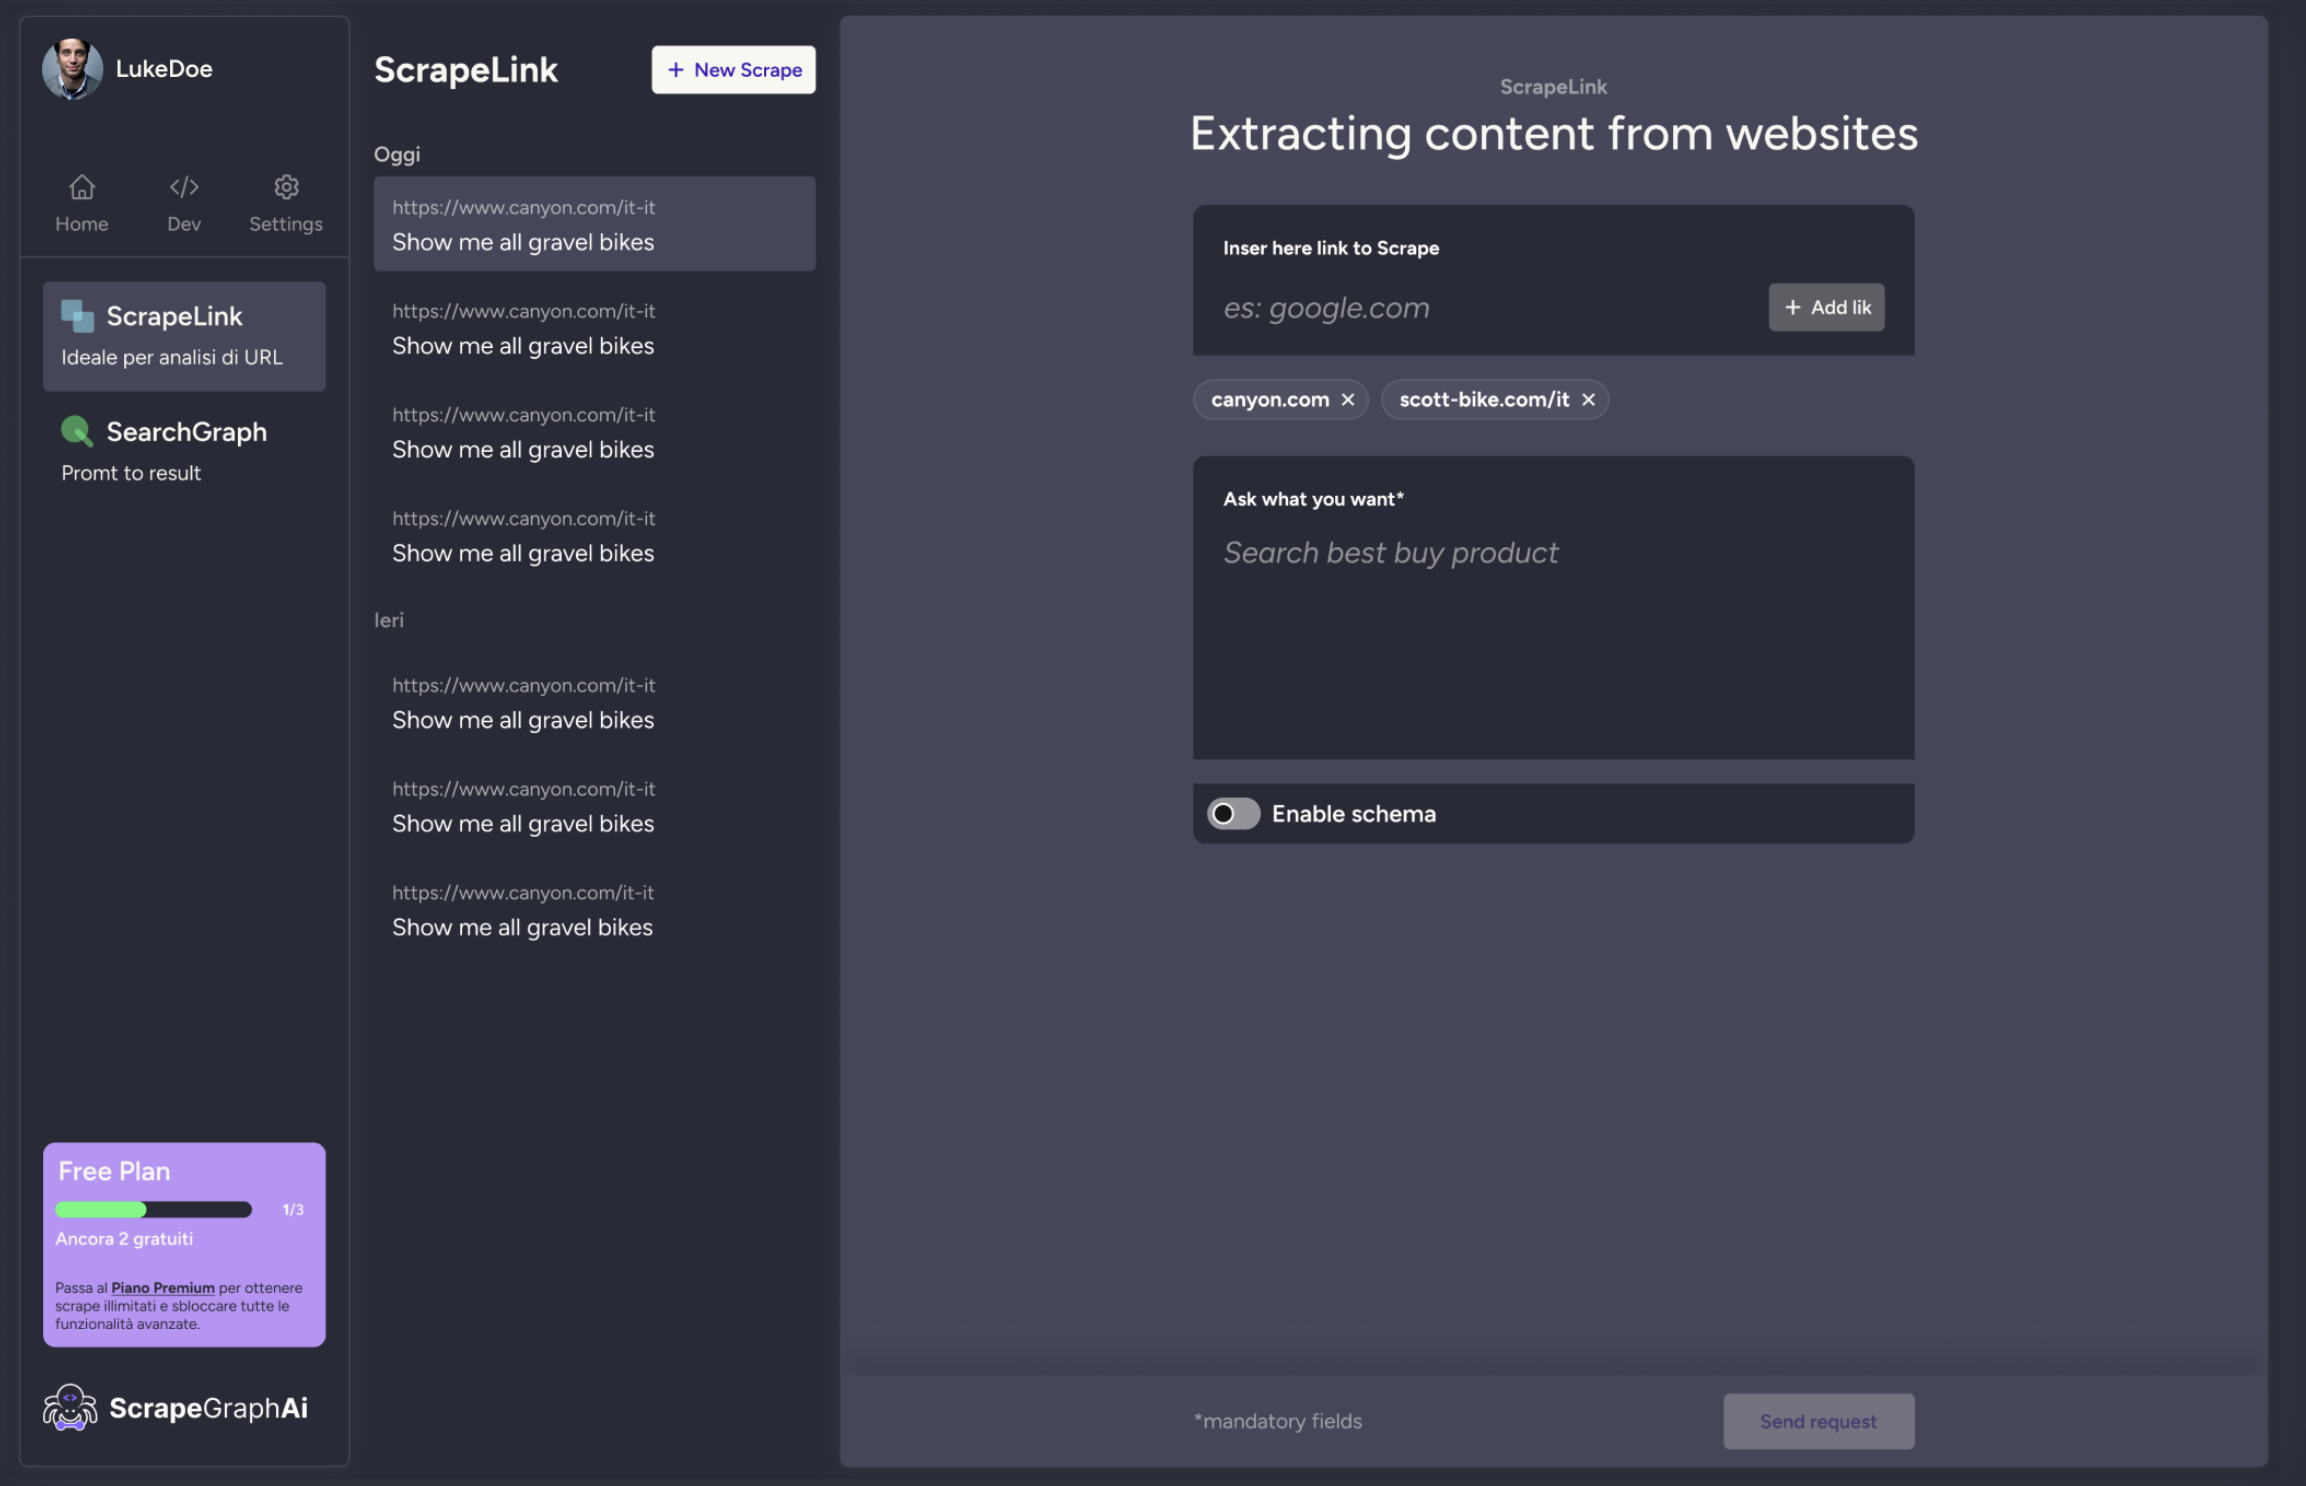
\includegraphics[width=1\linewidth]{Assets/webapp.png}
    \caption{First ScrapegraphAI  product}
    \label{fig:enter-label}
\end{figure}

At the end of Q3 2024, the ScrapegraphAI  library was named the second fastest-growing open-source library in the world, as reported by \cite{runacap2024}.

\begin{figure}[H]
    \centering
    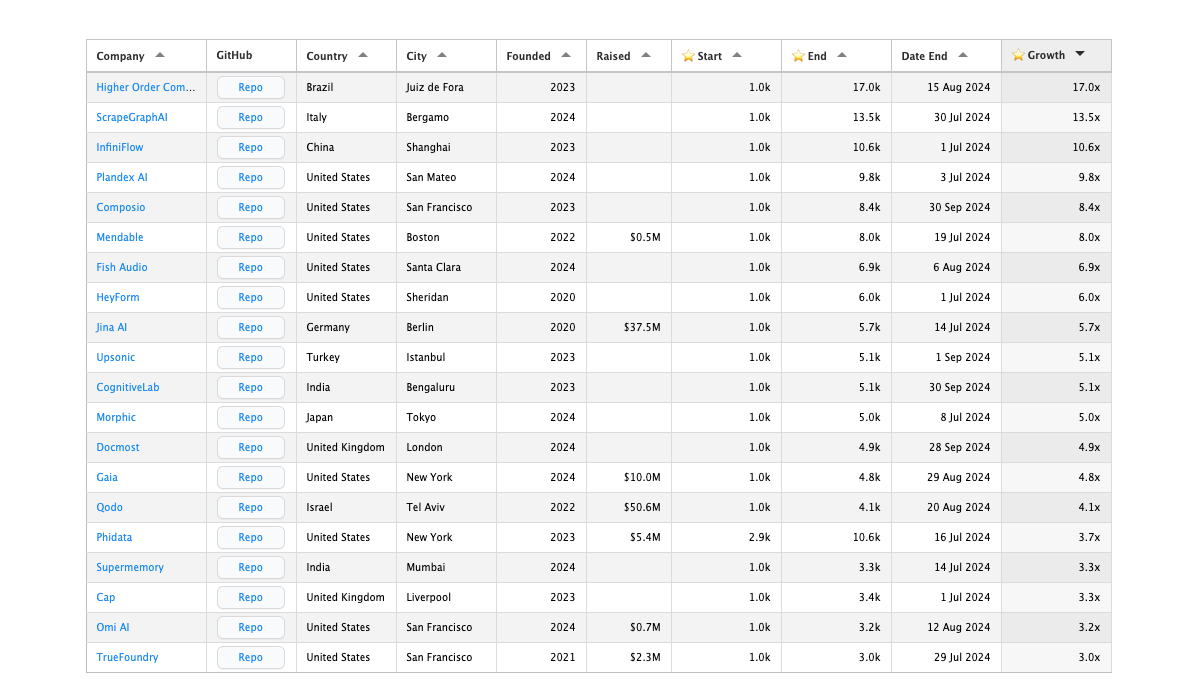
\includegraphics[width=0.95\linewidth]{growing_companies.png}
    \caption{Top trending open-source startups open table on 2024 Q3, source: runacap}
    \label{fig:enter-label}

\end{figure}

From december 2024 the previous project was updated to a product were it was possible to buy credits for scraping using APIS, this idea was done because many companies needed to extract data with the use of the AI.
The  first page of the SaaS is present in the image \ref{fig:enter-dashboard-basi}, where is possible to see avaible credits and copy the API key.
\begin{figure}[H]
    \centering
    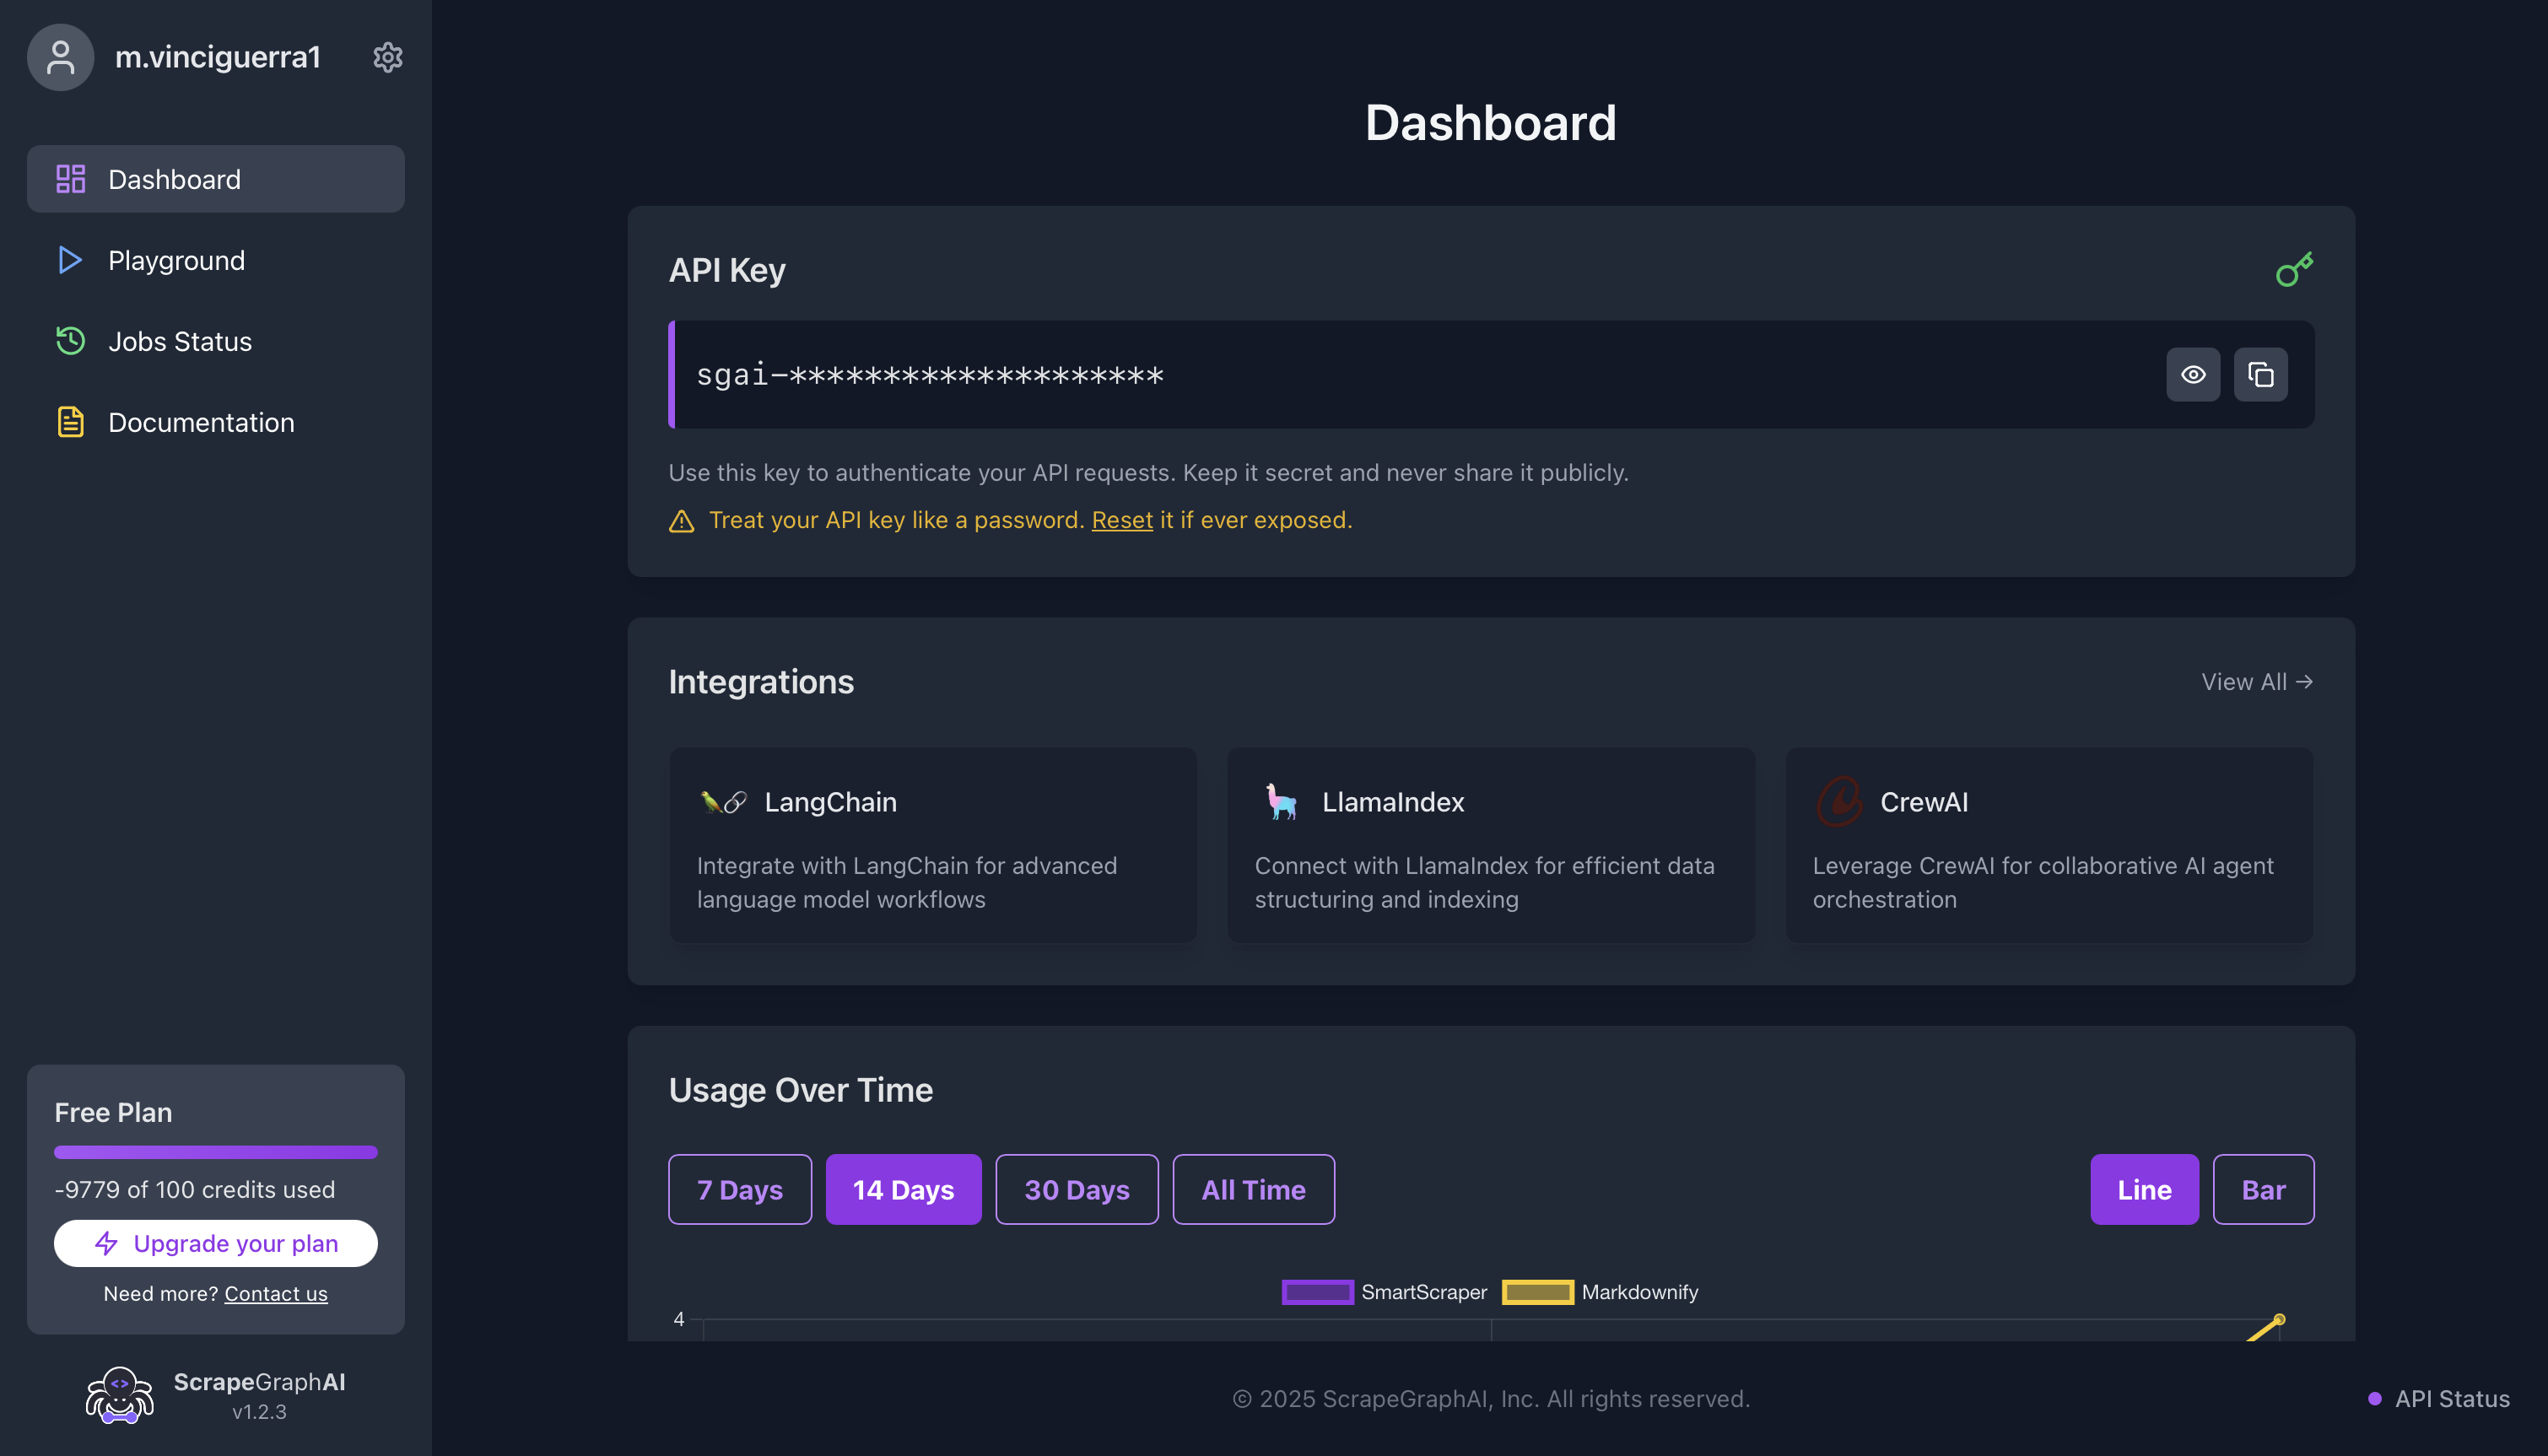
\includegraphics[width=0.95\linewidth]{Assets/dashboard_1.png}
    \caption{Dashboard basic page}
    \label{fig:enter-dashboard-basi}
\end{figure}

There is a second page, as it possbible to see in \ref{fig:enter-dashboard-playground} there is a playground where an user can try the apis
\begin{figure}[H]
    \centering
    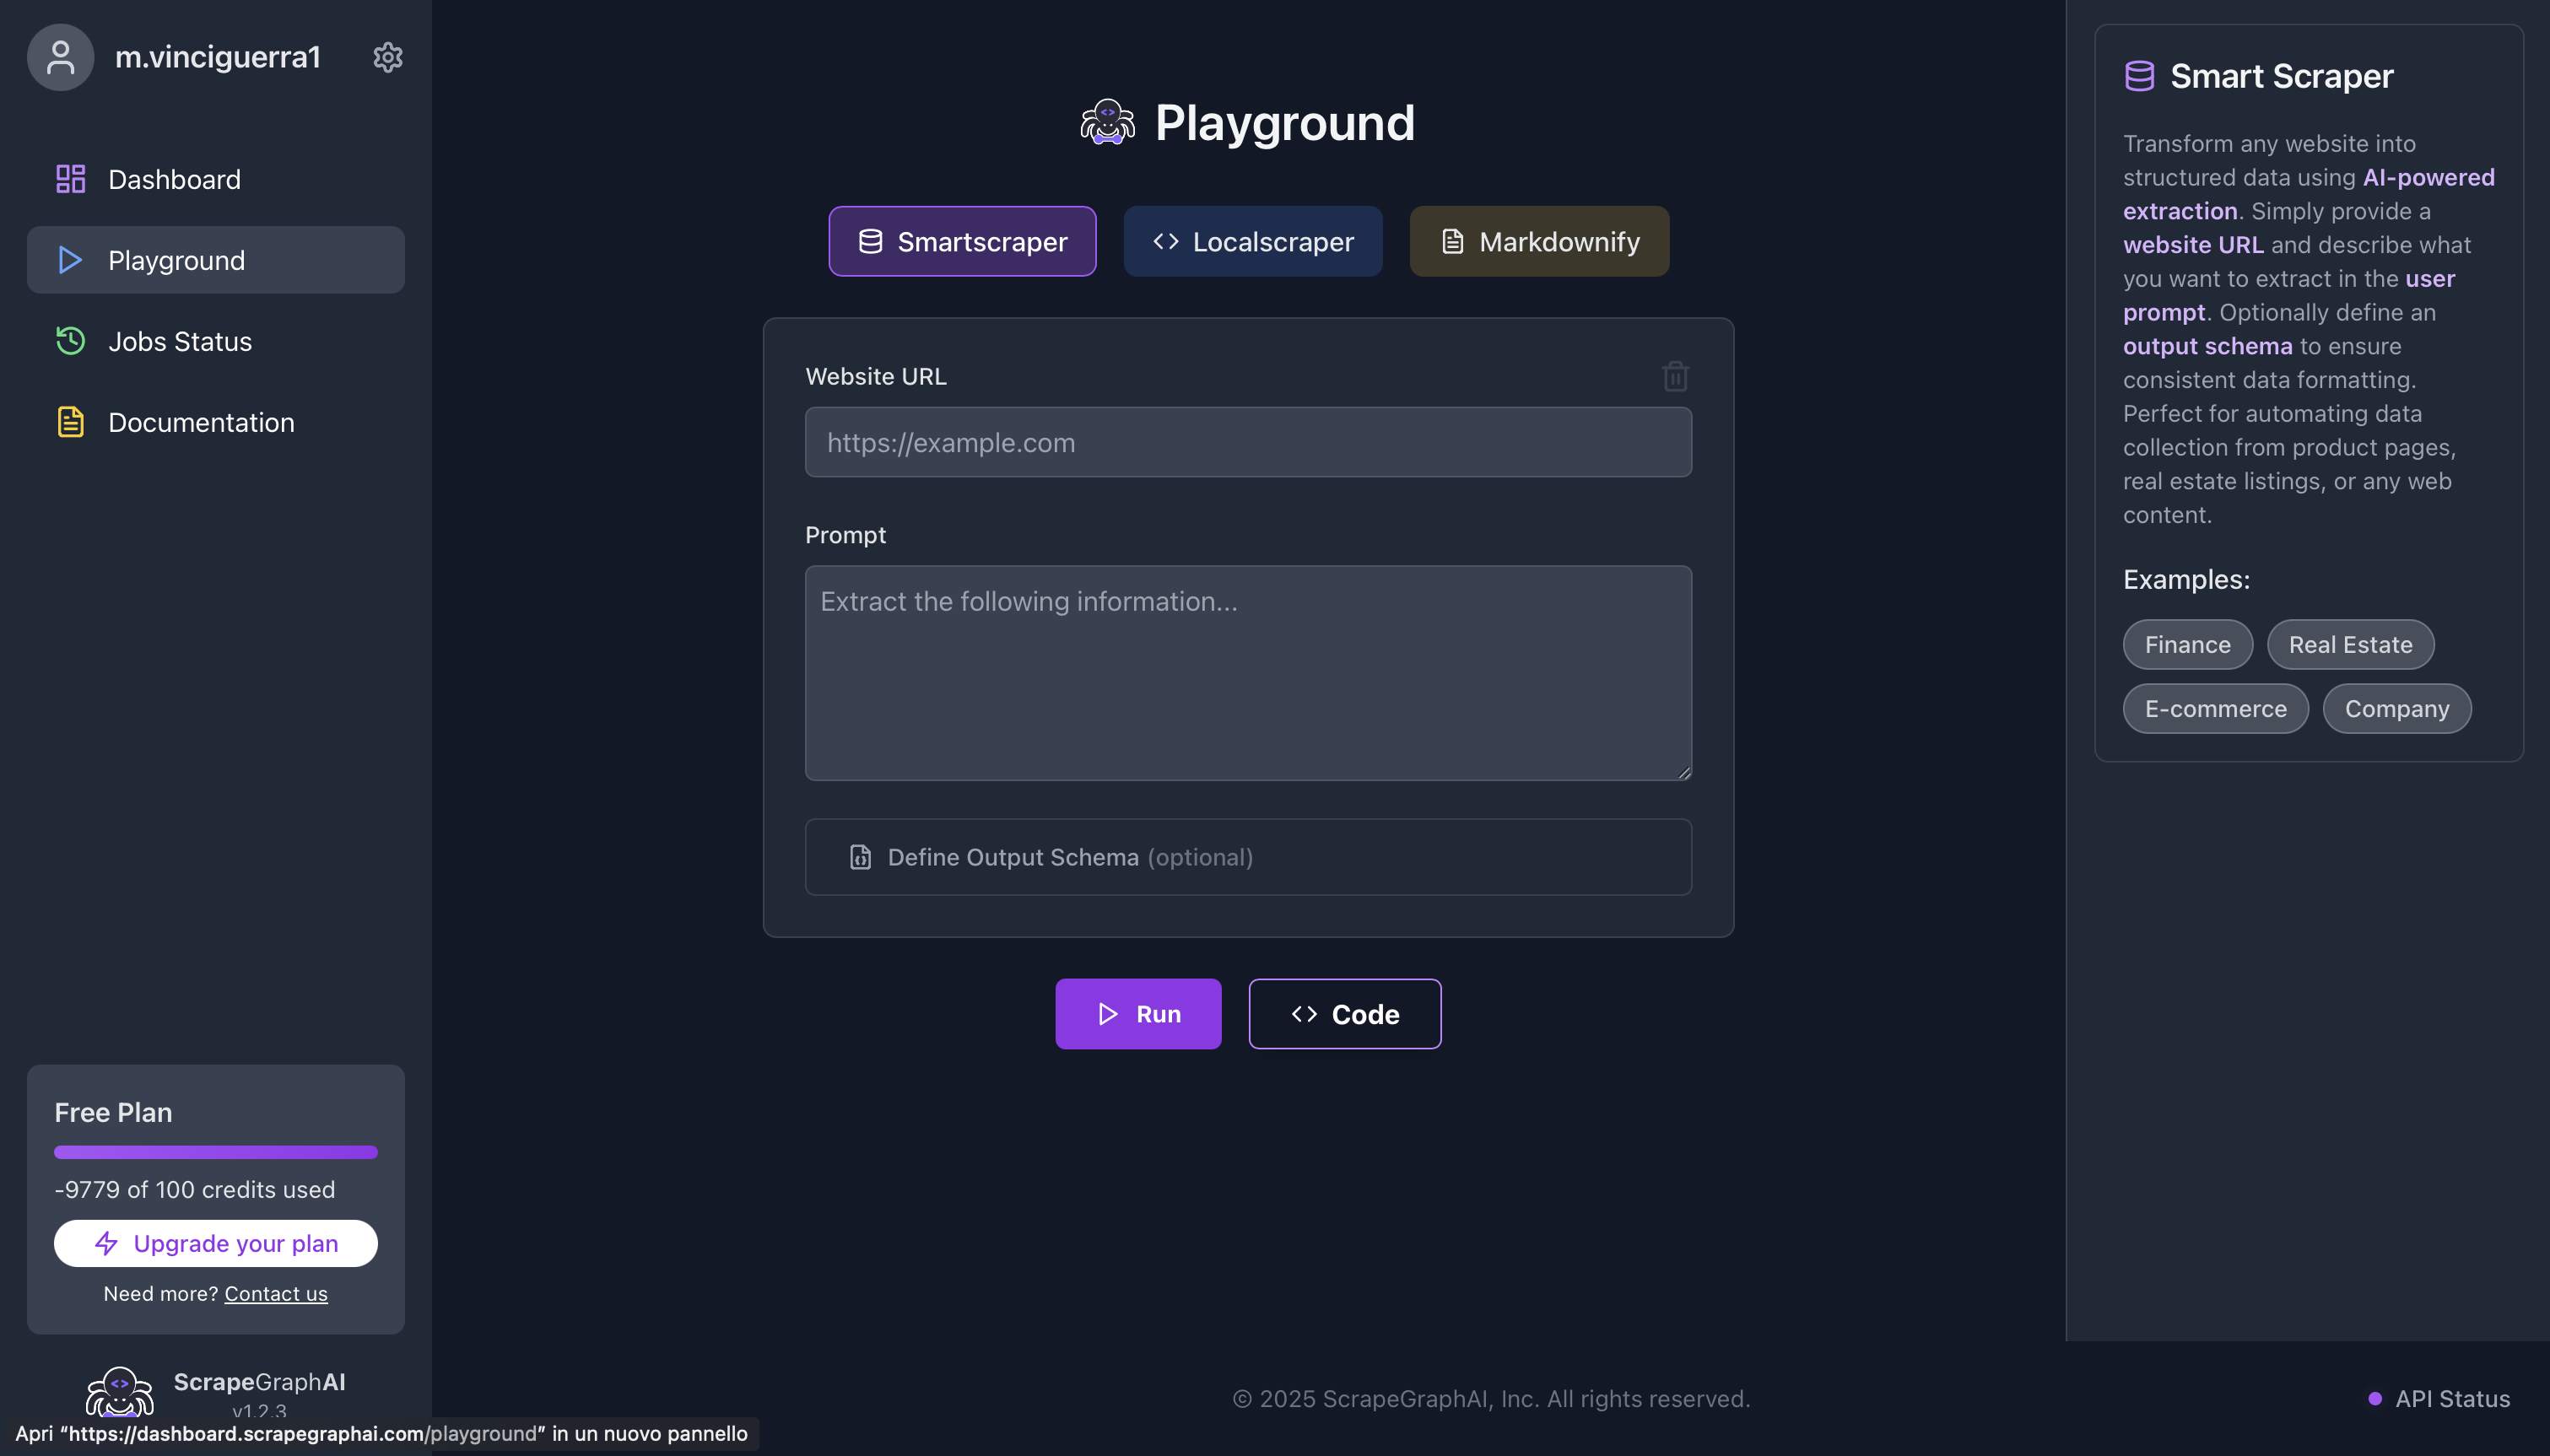
\includegraphics[width=0.95\linewidth]{Assets/dashboard_2.png}
    \caption{Dashboard playground}
    \label{fig:enter-dashboard-playground}
\end{figure}

And last, but not least, in the job status image \ref{fig:enter-dashboard-status} is it possible to see all the scraping result.
\begin{figure}[H]
    \centering
    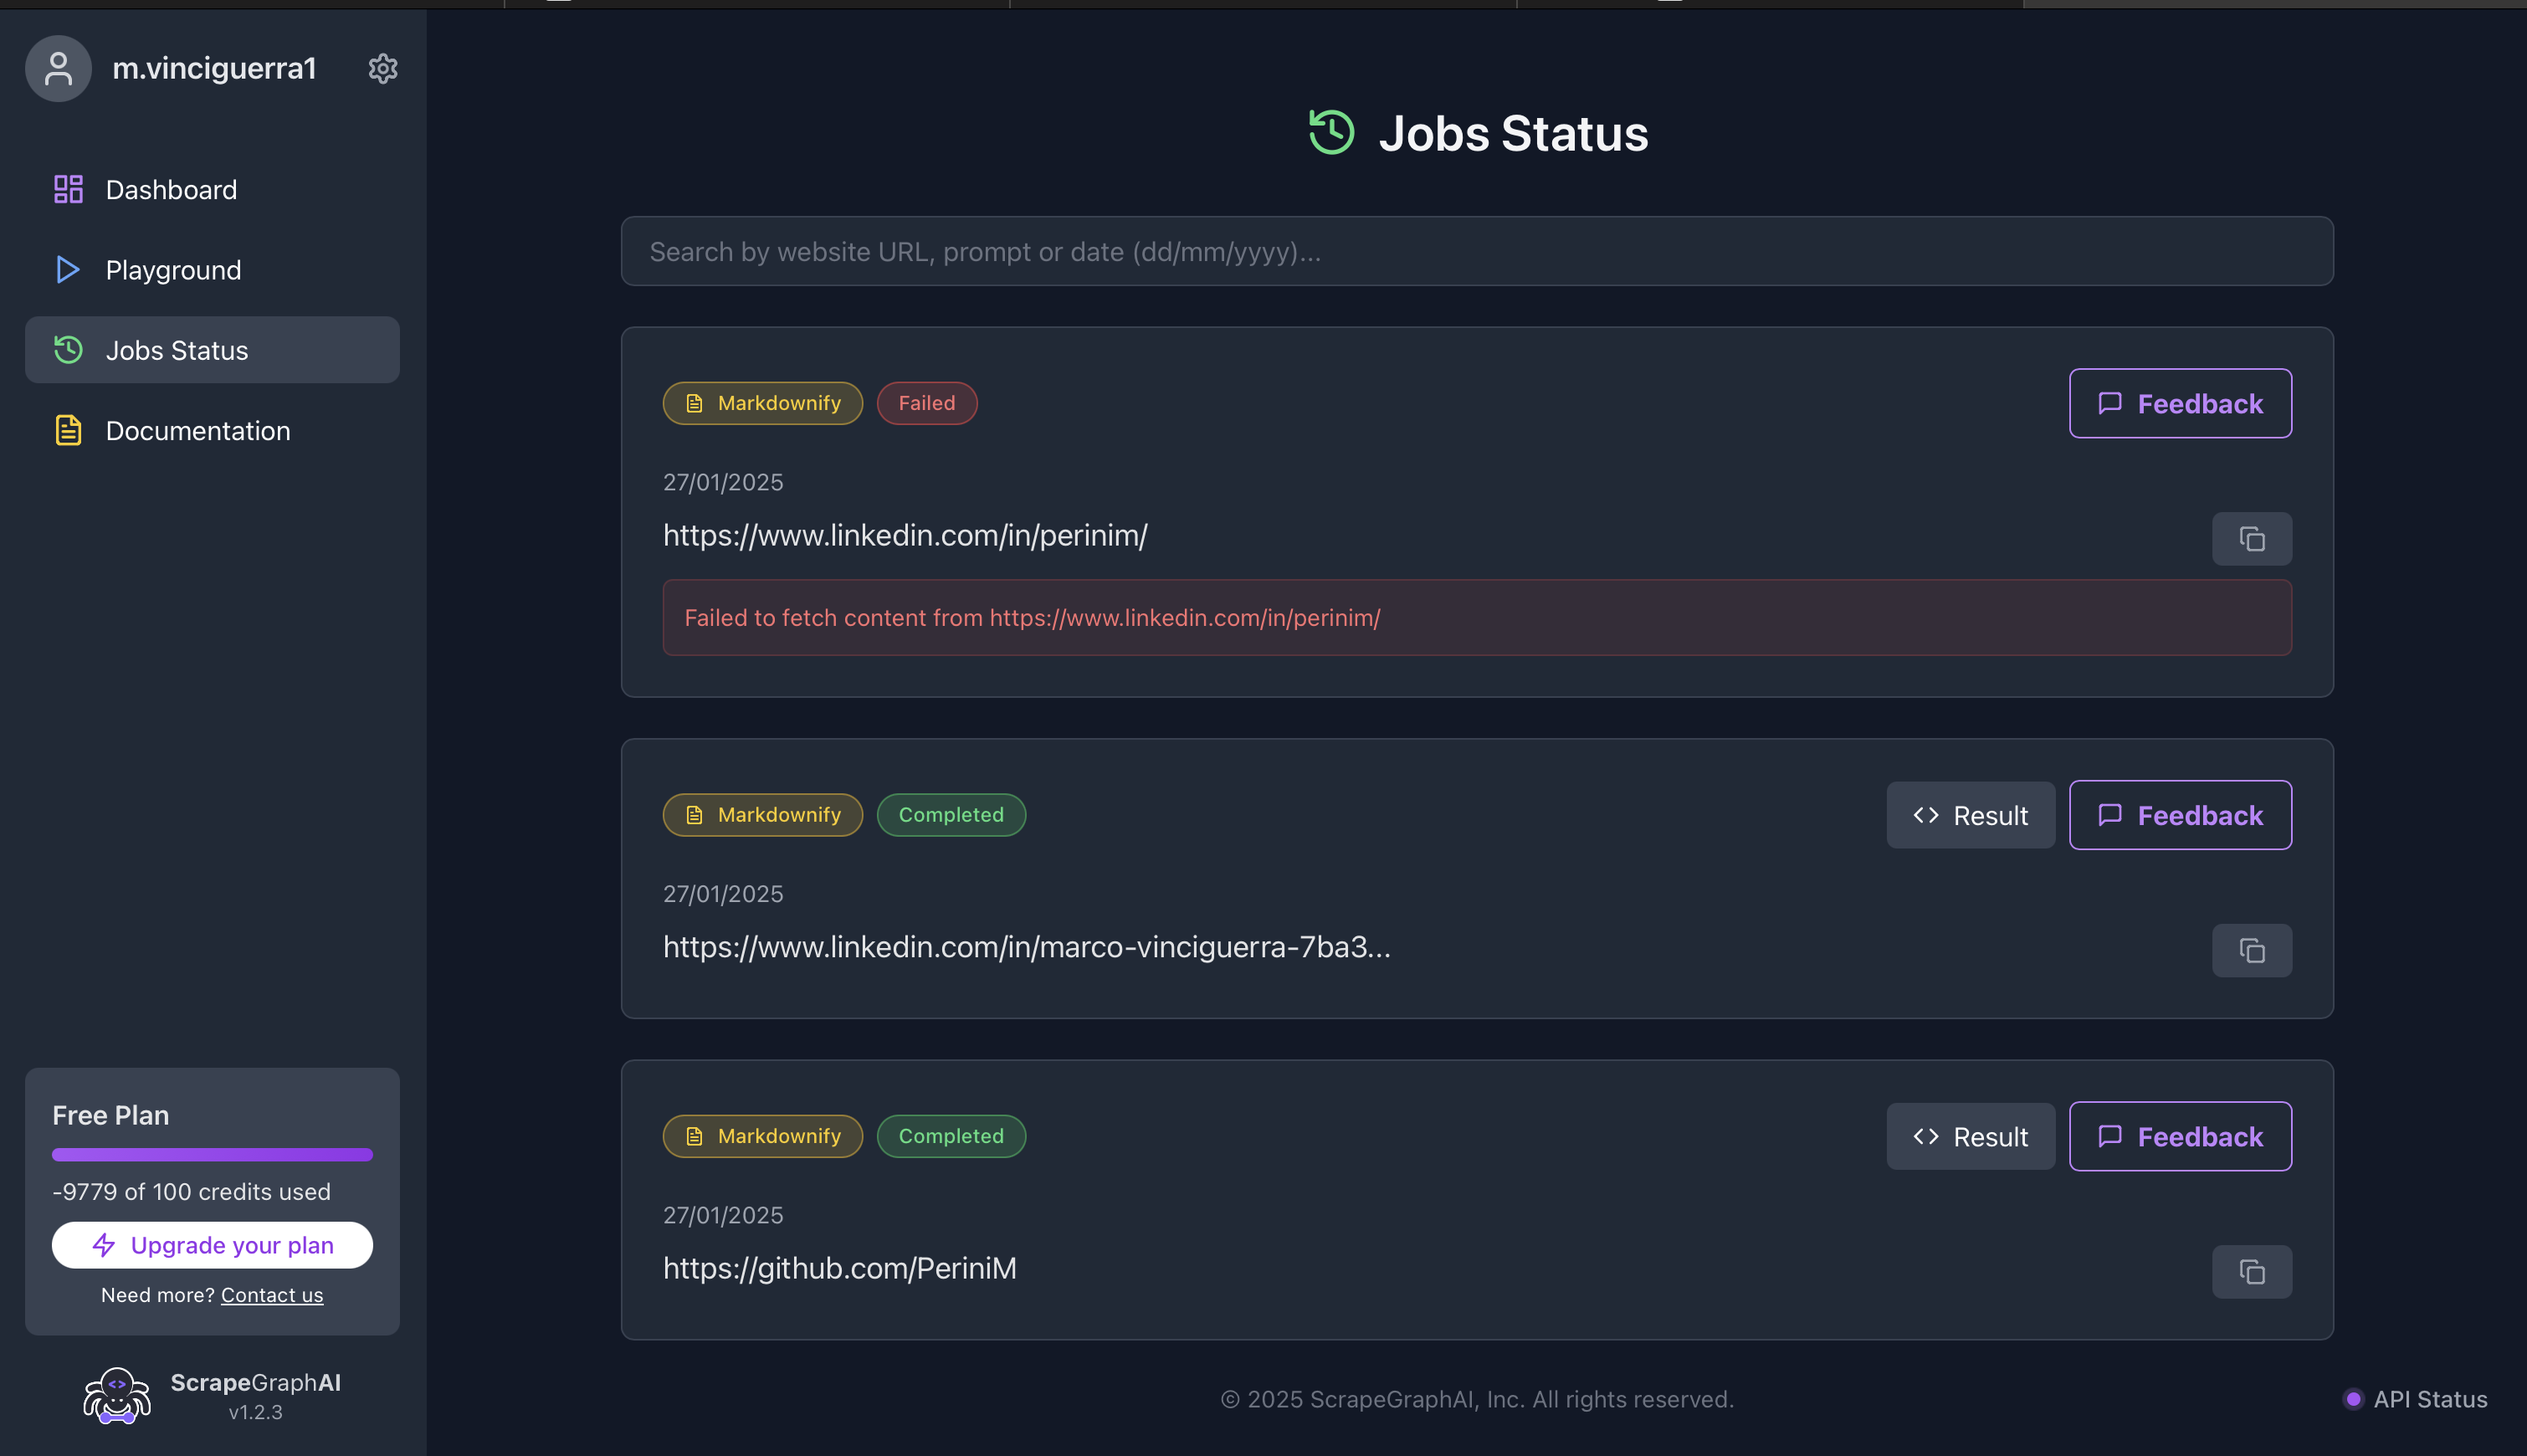
\includegraphics[width=0.95\linewidth]{Assets/dashboard_3.png}
    \caption{Dashboard job status}
    \label{fig:enter-dashboard-status}
\end{figure}

\section{Next steps}
\subsection{Integrations inside the agents}
Integrating ScrapegraphAI  into an agent-based environment enhances the ability of intelligent agents to effectively gather, process, and analyze web data at scale. ScrapegraphAI  provides advanced web scraping capabilities, combining speed, efficiency, and resilience against anti-scraping mechanisms. To incorporate ScrapegraphAI  in an agent's framework, developers must first set up the project dependencies in the pyproject.toml file by including the library under the dependencies section. Furthermore, the integration can be optimized by deploying ScrapeGraphA alongside LangGraph, which supports the seamless creation of agents capable of executing complex scraping workflows. The agent configuration, usually managed via Docker and Playwright, ensures that agents have a robust environment to manage interactions and scrape operations asynchronously. This modular approach allows for scalable and maintainable agent development tailored to large-scale web data extraction projects.

\subsection{Integration of RAG databases}
Retrieval Augmented Generation (RAG) is a technique used to enhance the performance of large language models (LLMs) by incorporating external information retrieval during text generation. Traditional language models generate responses based on pre-existing knowledge within their parameters, which can lead to errors or fabricated content (hallucinations) when faced with information beyond their training data. RAG addresses this by allowing the model to retrieve relevant external documents dynamically, thereby providing a foundation of accurate information for more reliable output \cite{jiang2023}.

In a typical RAG setup, the model first retrieves a set of documents relevant to the user’s query and then generates a response conditioned on the retrieved information. This single-step retrieval, though effective for short-form generation tasks, is limited when generating long, knowledge-intensive responses where continuous access to new information is required. To overcome this, Jiang et al. (2023) propose an iterative approach in RAG called Forward-Looking Active Retrieval (FLARE), where the model retrieves information at multiple points throughout the generation process. By anticipating the content needed for upcoming sentences, FLARE actively decides when and what to retrieve, resulting in higher accuracy for complex generation tasks such as long-form question answering and open-domain summarization \cite{jiang2023}.


\listoffigures
\listoftables


\bibliographystyle{siam}

\begin{thebibliography}{1}
\bibitem{1} Glez-Peña, Daniel, et al. "Web scraping technologies in an API world." Briefings in Bioinformatics 15.5 (2014): 788-797.
\bibitem{hirsch2014} 
Dennis D. Hirsch, ``The Glass House Effect: Big Data, the New Oil, and the Power of Analogy,'' \textit{Maine Law Review}, vol. 66, no. 2, 2014, pp. 373-396.

\bibitem{decker1997}
K. Decker, K. Sycara, and M. Williamson. Middle-agents for the Internet. In *Proceedings of the Fifteenth International Joint Conference on Artificial Intelligence (IJCAI)*, 1997.

\bibitem{abar2017}
    S. Abar, G. K. Theodoropoulos, P. Lemarinier, and G. M. P. O’Hare, ``Agent Based Modelling and Simulation tools: A review of the state-of-art software,'' \emph{Computer Science Review}, vol. 24, pp. 13–33, 2017.

\bibitem{azad2020} Azad, Babak Amin, et al. "Web Runner 2049: Evaluating Third-Party Anti-bot Services." \textit{DIMVA 2020, Lecture Notes in Computer Science}, vol. 12223, 2020, pp. 135–159. Springer, https://doi.org/10.1007/978-3-030-52683-2\_7.

\bibitem{schelen1998qosagents}
O. Schelén, \emph{Quality of Service Agents in the Internet}, Doctoral Thesis, Department of Computer Science and Electrical Engineering, Luleå University of Technology, 1998.

\bibitem{darmawan2022evaluating}
I. Darmawan, M. Maulana, R. Gunawan, and N. Widiyasono, ``Evaluating Web Scraping Performance Using XPath, CSS Selector, Regular Expression, and HTML DOM With Multiprocessing,'' \emph{International Journal on Informatics Visualization}, vol. 6, no. 4, pp. 904-910, 2022.

\bibitem{David2008}
P.~A. David and J.~S. Shapiro, ``Community-based production of open-source software: What do we know about the developers who participate?'' \emph{Information Economics and Policy}, vol.~20, no.~3, pp. 364–398, 2008.

  \bibitem{ahluwalia2023}
    A. Ahluwalia and S. Wani, ``Leveraging Large Language Models for Web Scraping,'' \emph{arXiv preprint arXiv:2406.08246v1}, 2023.
\bibitem{vaswani2017attention}
A. Vaswani, N. Shazeer, N. Parmar, J. Uszkoreit, L. Jones, A. N. Gomez, Ł. Kaiser, and I. Polosukhin, ``Attention is All You Need,'' \textit{Advances in Neural Information Processing Systems (NeurIPS)}, pp. 5998--6008, 2017.
 \bibitem{application_llms} Hadi, M. U., Tashi, Q. A., Shah, A., et al., "Large Language Models: A Comprehensive Survey of its Applications, Challenges, Limitations, and Future Prospects," TechRxiv, 2024

\bibitem{rasnayaka2024}
Rasnayaka, S., Wang, G., Shariffdeen, R., \& Iyer, G. N. (2024). An Empirical Study on Usage and Perceptions of LLMs in a Software Engineering Project. \textit{Proceedings of the 2024 International Workshop on Large Language Models for Code (LLM4Code ’24)}, April 20, Lisbon, Portugal. ACM, New York, NY, USA \url{https://doi.org/10.1145/3643795.3648379}.
\bibitem{limitations_llms} Hadi, M. U., Tashi, Q. A., Shah, A., et al., "Large Language Models: A Comprehensive Survey of its Applications, Challenges, Limitations, and Future Prospects," TechRxiv, 2024.

\bibitem{janssen2005} Janssen, M. A. (2005). Agent-Based Modelling. \textit{Internet Encyclopaedia of Ecological Economics}, Arizona State University.

\bibitem{janssen2005} Janssen, M. A., \& Ostrom, E. (2005). Empirically based, agent-based models. Ecology and Society, 10(2), 37.



\bibitem{ginart2024} Ginart, A. A., Kodali, N., Lee, J., Xiong, C., Savarese, S., \& Emmons, J. (2024). Asynchronous Tool Usage for Real-Time Agents. Salesforce AI Research.



\bibitem{ginart2024} Ginart, A., et al. (2024). Asynchronous Agents in Real-Time AI Systems. arXiv preprint arXiv:2312.04511.

\bibitem{chan2025}
A. Chan, K. Wei, S. Huang, N. Rajkumar, E. Perrier, S. Lazar, G. K. Hadfield, and M. Anderljung.
\newblock Infrastructure for AI Agents.
\newblock \emph{arXiv preprint arXiv:2501.10114}, 2025.

\bibitem{bigdatawire2024}
Big Data Wire. (2024, March 6). \textit{GenAI doesn’t need bigger LLMs, it needs better data}. \url{https://www.bigdatawire.com/2024/03/06/genai-doesnt-need-bigger-llms-it-needs-better-data/}

\bibitem{privacyos2024}
PrivacyOS. (2024). \textit{The 95\% of sanctions is triggered by an offense on personal data and consents}. \url{https://www.privacyos.com/en/the-95-of-sanctions-is-triggered-by-an-offense-on-personal-data-and-consents/}

\bibitem{webscraper2024}
WebScraper. A brief history of web scraping. Retrieved November 5, 2024, from \url{https://webscraper.io/blog/brief-history-of-web-scraping}

\bibitem{humby2006}
Humby, C. (2006). *Data is the new oil. It's valuable, but if unrefined it cannot really be used. It has to be changed into gas, and gasoline is used to power a car.*

\bibitem{McCulloch1943}
Warren S. McCulloch and Walter Pitts, 
"A logical calculus of the ideas immanent in nervous activity," 
\textit{The Bulletin of Mathematical Biophysics}, 
vol. 5, no. 4, pp. 115--133, Dec. 1943. 
DOI: \href{https://doi.org/10.1007/bf02478259}{10.1007/bf02478259}.

\bibitem{glez-pena2013} 
Daniel Glez-Peña, Ana Lourenço, Hugo López-Fernández, Miguel Reboiro-Jato, and Florentino Fdez-Riverola. 
\textit{Web scraping technologies in an API world}. Briefings in Bioinformatics, Vol. 15, No. 5, 788-797, 2013.

\bibitem{citeseerx2024}
CiteSeerX. (2024). \textit{The Growing Value of Private Data}. \url{https://citeseerx.ist.psu.edu/document?repid=rep1&type=pdf&doi=e4ae9f8b13fab5c5ce1e1e820b64bce196f60c53}

\bibitem{runacap2024}
Runacap's Ross Index. \emph{Q3 2024 Report on Fastest-Growing Open-Source Libraries}, 2024. \url{https://runacap.com/ross-index/q3-2024/}.


\bibitem{Morris1999} 
R.G.M. Morris, ``D.O. Hebb: The Organization of Behavior, Wiley: New York; 1949,'' \textit{Brain Research Bulletin}, vol. 50, no. 5-6, p. 437, Nov. 1999, doi: \href{https://doi.org/10.1016/s0361-9230(99)00182-3}{10.1016/s0361-9230(99)00182-3}.

\bibitem{LSTM}
S. Hochreiter and J. Schmidhuber, ``Long Short-term Memory,'' \textit{Neural Computation}, vol. 9, pp. 1735-80, Dec. 1997, doi: \href{https://doi.org/10.1162/neco.1997.9.8.1735}{10.1162/neco.1997.9.8.1735}.

\bibitem{gu2024} 
Y. Gu, L. Dong, F. Wei, and M. Huang, 
\textit{MiniLLM: Knowledge Distillation of Large Language Models}, 
Proceedings of ICLR 2024.
    
\bibitem{shreekumar2022importance}
Shreekumar, S., Mundke, S., \& Dhanawade, M. (2022). \textit{Importance of Web Scraping in E-Commerce Business}. NCRD’s Technical Review: e-Journal, 7(1). Sterling Institute of Management Studies.


 \bibitem{jiang2023}
    Z. Jiang, F. F. Xu, L. Gao, Z. Sun, Q. Liu, J. Dwivedi-Yu, Y. Yang, J. Callan, and G. Neubig, ``Active Retrieval Augmented Generation,'' \emph{arXiv preprint arXiv:2305.06983v2}, 2023.
\bibitem{hadi2024}
Hadi, M. U., Al Tashi, Q., Shah, A., et al. (2024). Large Language Models: A Comprehensive Survey of Its Applications, Challenges, Limitations, and Future Prospects. \textit{TechRxiv Preprints}. Retrieved from \url{https://doi.org/10.36227/techrxiv.23589741.v6}.




\bibitem{Tamburri2019}
D.~A. Tamburri, F.~Palomba, A.~Serebrenik, and A.~Zaidman, ``Discovering community patterns in open-source: A systematic approach and its evaluation,'' \emph{Empirical Software Engineering}, vol.~24, no.~3, pp. 1369–1417, 2019.


\end{thebibliography}




\bibliographystyle{siam}

\begin{thebibliography}{1}
\bibitem{1} Glez-Peña, Daniel, et al. "Web scraping technologies in an API world." Briefings in Bioinformatics 15.5 (2014): 788-797.
\bibitem{2} 
Dennis D. Hirsch, ``The Glass House Effect: Big Data, the New Oil, and the Power of Analogy,'' \textit{Maine Law Review}, vol. 66, no. 2, 2014, pp. 373-396.

\bibitem{3}
K. Decker, K. Sycara, and M. Williamson. Middle-agents for the Internet. In *Proceedings of the Fifteenth International Joint Conference on Artificial Intelligence (IJCAI)*, 1997.

\bibitem{4}
    S. Abar, G. K. Theodoropoulos, P. Lemarinier, and G. M. P. O’Hare, ``Agent Based Modelling and Simulation tools: A review of the state-of-art software,'' \emph{Computer Science Review}, vol. 24, pp. 13–33, 2017.

\bibitem{5} Azad, Babak Amin, et al. "Web Runner 2049: Evaluating Third-Party Anti-bot Services." \textit{DIMVA 2020, Lecture Notes in Computer Science}, vol. 12223, 2020, pp. 135–159. Springer, https://doi.org/10.1007/978-3-030-52683-2\_7.

\bibitem{6}
O. Schelén, \emph{Quality of Service Agents in the Internet}, Doctoral Thesis, Department of Computer Science and Electrical Engineering, Luleå University of Technology, 1998.

\bibitem{darmawan2022evaluating}
I. Darmawan, M. Maulana, R. Gunawan, and N. Widiyasono, ``Evaluating Web Scraping Performance Using XPath, CSS Selector, Regular Expression, and HTML DOM With Multiprocessing,'' \emph{International Journal on Informatics Visualization}, vol. 6, no. 4, pp. 904-910, 2022.

\bibitem{7}
P.~A. David and J.~S. Shapiro, ``Community-based production of open-source software: What do we know about the developers who participate?'' \emph{Information Economics and Policy}, vol.~20, no.~3, pp. 364–398, 2008.

  \bibitem{8}
    A. Ahluwalia and S. Wani, ``Leveraging Large Language Models for Web Scraping,'' \emph{arXiv preprint arXiv:2406.08246v1}, 2023.
\bibitem{9}
A. Vaswani, N. Shazeer, N. Parmar, J. Uszkoreit, L. Jones, A. N. Gomez, Ł. Kaiser, and I. Polosukhin, ``Attention is All You Need,'' \textit{Advances in Neural Information Processing Systems (NeurIPS)}, pp. 5998--6008, 2017.
 \bibitem{application_llms} Hadi, M. U., Tashi, Q. A., Shah, A., et al., "Large Language Models: A Comprehensive Survey of its Applications, Challenges, Limitations, and Future Prospects," TechRxiv, 2024

\bibitem{10}
Rasnayaka, S., Wang, G., Shariffdeen, R., \& Iyer, G. N. (2024). An Empirical Study on Usage and Perceptions of LLMs in a Software Engineering Project. \textit{Proceedings of the 2024 International Workshop on Large Language Models for Code (LLM4Code ’24)}, April 20, Lisbon, Portugal. ACM, New York, NY, USA \url{https://doi.org/10.1145/3643795.3648379}.
\bibitem{limitations_llms} Hadi, M. U., Tashi, Q. A., Shah, A., et al., "Large Language Models: A Comprehensive Survey of its Applications, Challenges, Limitations, and Future Prospects," TechRxiv, 2024.

\bibitem{11} Janssen, M. A. (2005). Agent-Based Modelling. \textit{Internet Encyclopaedia of Ecological Economics}, Arizona State University.

\bibitem{11} Janssen, M. A., \& Ostrom, E. (2005). Empirically based, agent-based models. Ecology and Society, 10(2), 37.



\bibitem{12} Ginart, A. A., Kodali, N., Lee, J., Xiong, C., Savarese, S., \& Emmons, J. (2024). Asynchronous Tool Usage for Real-Time Agents. Salesforce AI Research.



\bibitem{12} Ginart, A., et al. (2024). Asynchronous Agents in Real-Time AI Systems. arXiv preprint arXiv:2312.04511.

\bibitem{13}
A. Chan, K. Wei, S. Huang, N. Rajkumar, E. Perrier, S. Lazar, G. K. Hadfield, and M. Anderljung.
\newblock Infrastructure for AI Agents.
\newblock \emph{arXiv preprint arXiv:2501.10114}, 2025.

\bibitem{14}
Big Data Wire. (2024, March 6). \textit{GenAI doesn’t need bigger LLMs, it needs better data}. \url{https://www.bigdatawire.com/2024/03/06/genai-doesnt-need-bigger-llms-it-needs-better-data/}

\bibitem{15}
PrivacyOS. (2024). \textit{The 95\% of sanctions is triggered by an offense on personal data and consents}. \url{https://www.privacyos.com/en/the-95-of-sanctions-is-triggered-by-an-offense-on-personal-data-and-consents/}

\bibitem{16}
WebScraper. A brief history of web scraping. Retrieved November 5, 2024, from \url{https://webscraper.io/blog/brief-history-of-web-scraping}

\bibitem{17}
Humby, C. (2006). *Data is the new oil. It's valuable, but if unrefined it cannot really be used. It has to be changed into gas, and gasoline is used to power a car.*

\bibitem{McCulloch1943}
Warren S. McCulloch and Walter Pitts, 
"A logical calculus of the ideas immanent in nervous activity," 
\textit{The Bulletin of Mathematical Biophysics}, 
vol. 5, no. 4, pp. 115--133, Dec. 1943. 
DOI: \href{https://doi.org/10.1007/bf02478259}{10.1007/bf02478259}.

\bibitem{18} 
Daniel Glez-Peña, Ana Lourenço, Hugo López-Fernández, Miguel Reboiro-Jato, and Florentino Fdez-Riverola. 
\textit{Web scraping technologies in an API world}. Briefings in Bioinformatics, Vol. 15, No. 5, 788-797, 2013.

\bibitem{19}
CiteSeerX. (2024). \textit{The Growing Value of Private Data}. \url{https://citeseerx.ist.psu.edu/document?repid=rep1&type=pdf&doi=e4ae9f8b13fab5c5ce1e1e820b64bce196f60c53}

\bibitem{20}
Runacap's Ross Index. \emph{Q3 2024 Report on Fastest-Growing Open-Source Libraries}, 2024. \url{https://runacap.com/ross-index/q3-2024/}.


\bibitem{21} 
R.G.M. Morris, ``D.O. Hebb: The Organization of Behavior, Wiley: New York; 1949,'' \textit{Brain Research Bulletin}, vol. 50, no. 5-6, p. 437, Nov. 1999, doi: \href{https://doi.org/10.1016/s0361-9230(99)00182-3}{10.1016/s0361-9230(99)00182-3}.

\bibitem{22}
S. Hochreiter and J. Schmidhuber, ``Long Short-term Memory,'' \textit{Neural Computation}, vol. 9, pp. 1735-80, Dec. 1997, doi: \href{https://doi.org/10.1162/neco.1997.9.8.1735}{10.1162/neco.1997.9.8.1735}.

\bibitem{23} 
Y. Gu, L. Dong, F. Wei, and M. Huang, 
\textit{MiniLLM: Knowledge Distillation of Large Language Models}, 
Proceedings of ICLR 2024.
    
\bibitem{24}
Shreekumar, S., Mundke, S., \& Dhanawade, M. (2022). \textit{Importance of Web Scraping in E-Commerce Business}. NCRD’s Technical Review: e-Journal, 7(1). Sterling Institute of Management Studies.


 \bibitem{25}
    Z. Jiang, F. F. Xu, L. Gao, Z. Sun, Q. Liu, J. Dwivedi-Yu, Y. Yang, J. Callan, and G. Neubig, ``Active Retrieval Augmented Generation,'' \emph{arXiv preprint arXiv:2305.06983v2}, 2023.
\bibitem{hadi2024}
Hadi, M. U., Al Tashi, Q., Shah, A., et al. (2024). Large Language Models: A Comprehensive Survey of Its Applications, Challenges, Limitations, and Future Prospects. \textit{TechRxiv Preprints}. Retrieved from \url{https://doi.org/10.36227/techrxiv.23589741.v6}.




\bibitem{26}
D.~A. Tamburri, F.~Palomba, A.~Serebrenik, and A.~Zaidman, ``Discovering community patterns in open-source: A systematic approach and its evaluation,'' \emph{Empirical Software Engineering}, vol.~24, no.~3, pp. 1369–1417, 2019.


\end{thebibliography}



\end{document}
